% Options for packages loaded elsewhere
\PassOptionsToPackage{unicode}{hyperref}
\PassOptionsToPackage{hyphens}{url}
%
\documentclass[
]{article}
\usepackage{amsmath,amssymb}
\usepackage{lmodern}
\usepackage{iftex}
\ifPDFTeX
  \usepackage[T1]{fontenc}
  \usepackage[utf8]{inputenc}
  \usepackage{textcomp} % provide euro and other symbols
\else % if luatex or xetex
  \usepackage{unicode-math}
  \defaultfontfeatures{Scale=MatchLowercase}
  \defaultfontfeatures[\rmfamily]{Ligatures=TeX,Scale=1}
\fi
% Use upquote if available, for straight quotes in verbatim environments
\IfFileExists{upquote.sty}{\usepackage{upquote}}{}
\IfFileExists{microtype.sty}{% use microtype if available
  \usepackage[]{microtype}
  \UseMicrotypeSet[protrusion]{basicmath} % disable protrusion for tt fonts
}{}
\makeatletter
\@ifundefined{KOMAClassName}{% if non-KOMA class
  \IfFileExists{parskip.sty}{%
    \usepackage{parskip}
  }{% else
    \setlength{\parindent}{0pt}
    \setlength{\parskip}{6pt plus 2pt minus 1pt}}
}{% if KOMA class
  \KOMAoptions{parskip=half}}
\makeatother
\usepackage{xcolor}
\IfFileExists{xurl.sty}{\usepackage{xurl}}{} % add URL line breaks if available
\IfFileExists{bookmark.sty}{\usepackage{bookmark}}{\usepackage{hyperref}}
\hypersetup{
  pdftitle={Application of the Woods Hole Assessment Model to Black Sea Bass},
  pdfauthor={Timothy J. Miller\^{}\{1,*\}; Kiersten Curti\^{}1; Alex Hansell\^{}1},
  hidelinks,
  pdfcreator={LaTeX via pandoc}}
\urlstyle{same} % disable monospaced font for URLs
\usepackage[margin=1in]{geometry}
\usepackage{longtable,booktabs,array}
\usepackage{calc} % for calculating minipage widths
% Correct order of tables after \paragraph or \subparagraph
\usepackage{etoolbox}
\makeatletter
\patchcmd\longtable{\par}{\if@noskipsec\mbox{}\fi\par}{}{}
\makeatother
% Allow footnotes in longtable head/foot
\IfFileExists{footnotehyper.sty}{\usepackage{footnotehyper}}{\usepackage{footnote}}
\makesavenoteenv{longtable}
\usepackage{graphicx}
\makeatletter
\def\maxwidth{\ifdim\Gin@nat@width>\linewidth\linewidth\else\Gin@nat@width\fi}
\def\maxheight{\ifdim\Gin@nat@height>\textheight\textheight\else\Gin@nat@height\fi}
\makeatother
% Scale images if necessary, so that they will not overflow the page
% margins by default, and it is still possible to overwrite the defaults
% using explicit options in \includegraphics[width, height, ...]{}
\setkeys{Gin}{width=\maxwidth,height=\maxheight,keepaspectratio}
% Set default figure placement to htbp
\makeatletter
\def\fps@figure{htbp}
\makeatother
\setlength{\emergencystretch}{3em} % prevent overfull lines
\providecommand{\tightlist}{%
  \setlength{\itemsep}{0pt}\setlength{\parskip}{0pt}}
\setcounter{secnumdepth}{5}
\newlength{\cslhangindent}
\setlength{\cslhangindent}{1.5em}
\newlength{\csllabelwidth}
\setlength{\csllabelwidth}{3em}
\newlength{\cslentryspacingunit} % times entry-spacing
\setlength{\cslentryspacingunit}{\parskip}
\newenvironment{CSLReferences}[2] % #1 hanging-ident, #2 entry spacing
 {% don't indent paragraphs
  \setlength{\parindent}{0pt}
  % turn on hanging indent if param 1 is 1
  \ifodd #1
  \let\oldpar\par
  \def\par{\hangindent=\cslhangindent\oldpar}
  \fi
  % set entry spacing
  \setlength{\parskip}{#2\cslentryspacingunit}
 }%
 {}
\usepackage{calc}
\newcommand{\CSLBlock}[1]{#1\hfill\break}
\newcommand{\CSLLeftMargin}[1]{\parbox[t]{\csllabelwidth}{#1}}
\newcommand{\CSLRightInline}[1]{\parbox[t]{\linewidth - \csllabelwidth}{#1}\break}
\newcommand{\CSLIndent}[1]{\hspace{\cslhangindent}#1}
\usepackage{url}
\usepackage{setspace}
%\singlespacing
%\onehalfspacing
%\doublespacing
\usepackage{lineno}
%\linenumbers
\usepackage[belowskip=0pt,aboveskip=0pt]{caption}
\usepackage{relsize}
\usepackage{float}
% \usepackage[section]{placeins}
\usepackage{lscape}
\newcommand{\blandscape}{\begin{landscape}}
\newcommand{\elandscape}{\end{landscape}}
\usepackage{booktabs}
\usepackage{longtable}
\usepackage{array}
\usepackage{multirow}
\usepackage{wrapfig}
\usepackage{float}
\usepackage{colortbl}
\usepackage{pdflscape}
\usepackage{tabu}
\usepackage{threeparttable}
\usepackage{threeparttablex}
\usepackage[normalem]{ulem}
\usepackage{makecell}
\usepackage{xcolor}
\ifLuaTeX
  \usepackage{selnolig}  % disable illegal ligatures
\fi

\title{Application of the Woods Hole Assessment Model to Black Sea Bass}
\author{Timothy J. Miller\(^{1,*}\) \and Kiersten Curti\(^1\) \and Alex Hansell\(^1\)}
\date{09 November, 2023}

\begin{document}
\maketitle

\(^1\)Northeast Fisheries Science Center, National Marine Fisheries Service, 166 Water Street, Woods Hole, MA 02543, USA\\
\(^*\)Contact info: \href{mailto:timothy.j.miller@noaa.gov}{\nolinkurl{timothy.j.miller@noaa.gov}}

\pagebreak

\hypertarget{summary}{%
\section*{Summary}\label{summary}}
\addcontentsline{toc}{section}{Summary}

The Woods Hole Assessment Model (WHAM) software package is maintained and developed at the Northeast Fisheries Science Center to enable state-space stock assessments, i.e.~where processes such as recruitment, the annual transitions in numbers-at-age (survival), natural mortality, selectivity, and catchability are treated as time- and, in some cases, age-varying random effects.

The proposed base model configuration for management uses a multi-stock, multi-region extension of WHAM (hereafter referred to as Multi-WHAM) to model the northern and southern components of the stock and movement of the northern component simultaneously. Multi-WHAM does not yet have the ability to use tagging data to inform the model, so it uses estimates of movement parameters from a Stock Synthesis application to define prior distributions for movement rates which are treated as random effects. VAST and Recreational catch per angler indices for the northern and southern regions along with corresponding age composition data are used to inform the model. Catch and associated age composition data for regional recreational and commercial fleets are also used. The model also includes effects of a winter bottom temperature covariate in the northern region on recruitment of the stock component in that region. Process errors in the latent bottom temperature covariate, recruitment, survival, and selectivity of some fleets and indices are estimated as random effects.

We arrived at the proposed base model from analyzing more than 30 different fits using Multi-WHAM with different sets of observations. The proposed base model exhibits negligible retrospective patterns in fishing mortality (Mohn's \(\rho\) = 0.058 and -0.045 for northern and southern regions, respectively) or SSB (Mohn's \(\rho\) = -0.054 and -0.007 for northern and southern components, respectively). OSA residuals appear adequate for most of the data components. Reference point estimates suggest the slight overfishing of the entire stock, but that the stock is far from overfished. Example 3 year projections are also provided.

\pagebreak

\hypertarget{introduction}{%
\section{Introduction}\label{introduction}}

Black sea bass is currently assessed using ASAP, the Age-Structured Assessment Program (Legault and Restrepo, 1998; Miller and Legault, 2015). ASAP is a statistical catch-at-age (SCAA) model which estimates all model parameters as fixed effects. The standard version of the Woods Hole Assessment Model can only be applied to a single stock and area Miller and Stock (2020). Here we use a multi-stock, multi-region extension of WHAM (\url{https://github.com/timjmiller/wham/tree/lab}, Miller, 2023, Multi-WHAM) for black sea bass originating and spawning in northern and southern regions of the US NE Shelf divided by the Hudson Canyon.

\hypertarget{methods}{%
\section{Methods}\label{methods}}

All code used for model fits along with results summaries can be found at \url{https://github.com/kcurti/BSB.2023.RT.Modeling}.

\hypertarget{early-runs}{%
\subsection{Early runs}\label{early-runs}}

The development of Multi-WHAM was driven primarily by the needs of black sea bass and NEUS stocks of Atlantic cod. Because this extension to WHAM represents a major change to the code used to configure and estimate models, we compared results from fits of separate ASAP models to both separate fits using the standard WHAM model for each region, as well as simultaneous fits of the regional components Multi-WHAM without any movement (Figure \ref{fig:compare-asap-wham}). All WHAM fits assumed no random effects and estimated annual recruitment parameters as fixed effects. Estimates from the Multi-WHAM fit and those from fits using the standard WHAM model provide identical results, but ASAP fits provide small differences in estimates for the northern component.

\hypertarget{model-configurations}{%
\subsection{Model configurations}\label{model-configurations}}

The first 18 runs that used updated and new observations included either separate indices for all surveys or fall and spring VAST indices that combined all surveys other than the recreational CPA (Table \ref{tab:wham-runs}). Many of these runs explored alternative selectivity and age composition assumptions to reduce patterns observed in the One-Step-Ahead (OSA) residuals for age composition observations. During the development of the first 18 model runs, the working group extensively discussed whether the preferred model should include individual state and federal trawl survey indices or aggregate indices developed through VAST modeling. Due to the interactions of the limited geographic footprint of many of the surveys with the black sea bass seasonal migration patterns, the working group concluded that the aggregate VAST indices that account for changes in catchability should be used in the proposed model.
We then found that the age composition for fall FAST and NEAMAP indices were incorrectly calculated. Then from Run 19 onward we only used the spring VAST and Recreational CPA indices.

From Run 19-27 we still had issues reducing patterns in OSA residuals and sometimes large patterns in retrospective patterns for the northern component. We then decided to iterate among alternative assumptions about selectivity and age composition models with the northern and southern components separately to resolve diagnostic problems more efficiently. These analyses resulted in different age composition model assumptions for different fleets and indices and the use of selectivity random effects for the northern fleets and indices (Table \ref{tab:age-comp-sel-table}).

Runs 28-34 largely used these same assumptions. These last runs used more realistic assumptions about movement and more appropriate usage of the estimates from the stock synthesis runs (Fay and McNamee, 2023). Run 31 assumed temporal random effects on the movement rate from the north to the south and Run 32 assumed a Beverton-Holt stock recruit relationships for both the north and south components, but convergence was problematic for both of these models. Run 33 investigated bottom temperature effects on recruitment and we found evidence of an effect on northern recruitment. Run 34 then relaxed an assumption common to many earlier runs about the estimated uncertainty in the Recreational CPA indices and allowed a scalar to be estimated in the model. Further details of model configuration of Runs 28-34 are described below.

\hypertarget{seasonality-and-movement}{%
\subsection{Seasonality and movement}\label{seasonality-and-movement}}

Th proposed base model assumes 11 intervals within each calendar year: 5 monthly time intervals from Jan 1 to May 31, a spawning season from June 1 to July 31, and 5 monthly intervals from August 1 to December 31. All southern fish are assumed to never move to the northern region. Northern fish are all in the northern region during the spawning period. A proportion \(p_1\) of northern fish can move to the south each month during the last 5 months of the year, but no movement is allows from the south to the north during this period. For the first 4 months of the year a proportion \(p_2\) of northern fish in the south can move back to the north, but no movement from the north to south is allowed during this period. In the fifth month any northern fish still in the south are assumed to move back to the north for the subsequent spawning period. We configured survival and movement to occur sequentially in each interval. Each of the two proportions are assumed constant across intervals, age, and year.

The monthly movement matrices are
\begin{equation*}
\mathbf{p}_{1} = 
  \begin{bmatrix}
     1-p_1 & p_1 \\
     0 & 1 \\
  \end{bmatrix}
\end{equation*}
for the portion of the year after spawning and
\begin{equation*}
\mathbf{p}_{2} = 
  \begin{bmatrix}
     1 &  0 \\
     p_2 & 1-p_2 \\
  \end{bmatrix}
\end{equation*}
for the portion of the year before spawning.

\hypertarget{prior-distribution-for-movement-rates}{%
\subsubsection{Prior distribution for movement rates}\label{prior-distribution-for-movement-rates}}

The Stock Synthesis model has 2 seasons (6 months each) where a proportion \(P_1\) of the northern component moves to the south in one season and some proportion \(P_2\) move back to the south in the second season (Fay and McNamee, 2023). The movement matrices for each season is
\begin{equation*}
\mathbf{P}_{1} = 
  \begin{bmatrix}
     1-P_1 & P_1 \\
     0 & 1 \\
  \end{bmatrix}
\end{equation*}
and
\begin{equation*}
\mathbf{P}_{2} = 
  \begin{bmatrix}
     1 &  0 \\
     P_2 & 1-P_2 \\
  \end{bmatrix}.
\end{equation*}

We approximate the monthly movement matrices as the roots \(\mathbf{P}_1\) and \(\mathbf{P}_2\) defined by the number of months of movement for each season (5 and 4, respectively): \(\mathbf{p}_1 = \mathbf{P}_1^{\frac{1}{5}}\) and \(\mathbf{p}_2 = \mathbf{P}_2^{\frac{1}{4}}\). Given the proportion parameter, the eigen decomposition of the matricies can be used to define the roots
\[  \mathbf{P}_1^{1/5} = \mathbf{V}_1 \mathbf{D}_1^{\frac{1}{5}} \mathbf{V}_1^{-1}\]
\[  \mathbf{P}_2^{1/4} = \mathbf{V}_2 \mathbf{D}_2^{\frac{1}{4}} \mathbf{V}_2^{-1}\]
where \(\mathbf{V}_i\) and \(\mathbf{D}_i\) are the matrix of eigenvectors (columnwise) and the diagonal matrix of corresponding eigenvalues of \(\mathbf{P}_i\) for parameter \(P_i\). Note, for diagonal matrices, \(\mathbf{D}_i^k\) is equal to the diagonal matrix with the elements raised to the power \(k\).

We used a parametric bootstrap approach to determine an appropriate standard deviation for the prior distribution for the movement parameters.
The actual SS parameter estimates \(x_1=-1.44\) and \(x_2=1.94\) are transformations of \(P_1=0.11\) and \(P_2=0.78\) such that
\[
P_i = \frac{1}{1 + 2e^{-x_i}}
\]
InMulti-WHAM an additive logit transformation is used which is simply a logit transformation when there are only two regions:
\[
p_i = \frac{1}{1+e^{-y_i}}.
\]
We simulated 1000 values from a normal distribution with mean and standard deviation defined by the SS parameter estimate and standard error \(\tilde x_i \sim N(x_i, SE(x_i))\). For each simulated value we constructed \(\mathbf{P}_i\), took the appropriate root and calculated inverse logit for \(\tilde y_i\). We calculated the mean and standard deviation of the values \(y_i\). The mean values did not differ meaningfully from the transformation of the original estimates (\(y_1 = -3.79\) and \(y_2 = -0.79\)) and the standard deviation was approximately 0.2 for both parameters.

\hypertarget{initial-abundance-at-age}{%
\subsection{Initial abundance at age}\label{initial-abundance-at-age}}

With the movement configuration, the northern origin fish (ages 2+) can occur in the southern region on January 1. Estimating initial numbers at age as separate parameters can be challenging even in single-stock models. To avoid challenges with estimating initial numbers at age in each region for the northern component in the two stock model, we used the equilibrium assumption described in Miller (2023). Using this assumption two parameters are estimated for each regional component: an initial recruitment and an equilibrium full F across all fleets.

\hypertarget{recruitment-and-survival}{%
\subsection{Recruitment and Survival}\label{recruitment-and-survival}}

For the northern population abundance at age 1 on January 1 (recruitment) is only allowed in the northern region, but given the monthly movement described above, older individuals that previously recruited in the northern region may occur in the southern region on January 1. Therefore, a model with survival random effects will model the transitions (survival/movement) of abundances at age of northern origin fish in each region. All of the initial runs assumed variance parameters for these random effects to be the same for northern origin fish occurring in both regions on January 1. The base model assumes very small variance for the transitions of northern fish in the southern region, which is essentially the same as the deterministic transition assumptions of a statistical catch at age model. We also allow 2DAR1 correlation for recruitment and survival for both the northern and southern components. Variance and correlation parameters for the recruitment and survival random effects are different for the northern and southern components.

\hypertarget{uncertainty-recreational-cpa-index-observations}{%
\subsection{Uncertainty recreational CPA index observations}\label{uncertainty-recreational-cpa-index-observations}}

The CVs provided by the analyses for the recreational catch per angler (RecCPA) ranged between 0.02 and 0.06 which the working group felt did not capture the true uncertainty in the index with regard to its relationship to stock abundance. In many of the initial runs as well as the base model we allowed a scalar multiple of the standard deviation of the log aggregate index to be estimated for these indices in the northern and southern regions. Models that successfully estimated these scalars indicated standard deviations for these surveys to be approximately 5 times the input value and this value was fixed in many preliminary runs to avoid dealing with convergence problems. However, the base model successfully estimated these scalars. The model estimates are negligibly affected by estimating these scalars, but we felt estimating these parameters allowed uncertainty in model output to be more properly conveyed.

\hypertarget{bottom-temperature-effects-on-recruitment}{%
\subsection{Bottom Temperature effects on recruitment}\label{bottom-temperature-effects-on-recruitment}}

We have bottom temperature observations for the northern and southern regions from 1963 to 2021 and estimated standard errors of those observations (Tabandera et al., 2023). We assumed AR1 models for the latent bottom temperature covariates in each region which are relatively precise with standard errors ranging between 0.03 and 0.09 degrees Celsius. We fit models with the bottom temperature covariate observations in the model, but without effects on recruitment. This is the null model which can be compared with models with effects on recruitment using AIC because the observations included in each model are the same. We fit models with effects of the regional bottom temperatures on both the respective stock components and just effect of the northern bottom temperature covariate on recruitment of the northern stock. These analyses derive from the hypothesis that bottom temperature affects overwinter survival of fish where the fish turn from age 0 to age 1 on January 1 (Miller et al., 2016).

We assume the covariate in year \(y\) affects recruitment in the same years because the covariate observations are from months January to March. The fish are technically already 1 year old, but there are no observations of these individuals until later in the year except possibly in fishery catches which are accumulated over the whole year. Expected log-recruitment is a linear function of log-recruitment at the previous time step and bottom temperature

\begin{equation}\label{eq:expected-recruitment}
\log R_y = \mu_R + \beta x_y + \epsilon_y
\end{equation}

\hypertarget{diagnostics}{%
\subsection{Diagnostics}\label{diagnostics}}

\hypertarget{jitter-analysis}{%
\subsubsection{Jitter analysis}\label{jitter-analysis}}

For this analysis we simulated fixed effects parameter vectors from a normal distribution with mean equal to the optimized values and covariance equal to the hessian-based covariance matrix. From refitting the model starting at 16 different simulated parameter vectors, we found 3 cases with a lower (\textasciitilde2 units) marginal negative log likelihood (Figure \ref{fig:jitter-res-1}). The gradients at these optimized values were satisfactory and there was no difference in parameter value among the 3 lower optimizations. In 1 of the 16 iterations, the model did not optimized satisfactorily, and in the other 12 iterations, the optimized marginal negative log-likelihood and parameter estimates were identical to the original fit. The parameters with estimates that differed most between the 2 optimization results were those associated with age composition observation dispersion parameters.

Given the revised model fit with the lower marginal NLL, we used the same jittering method with 100 simulated parameter values as starting values (Figure \ref{fig:jitter-res-2}). Three of the fits failed to complete, but none of the iterations resulted in lower marginal negative log-likelihood than that from the revised model estimates. Three of the fits minimized to greater marginal NLLs, but the gradients indicate lack of convergence. \textbf{The revised model fit is the proposed base model.}

\hypertarget{self-tests}{%
\subsubsection{Self tests}\label{self-tests}}

We performed a simulation self-test where new observations were simulated conditional on all random effects estimated in the proposed base model and the same model configuration was fit to each of the simulated data sets. For only 6 of the 100 simulated data sets, was the maximum absolute gradient for the fitted model was less than \(1\times10^{-6}\). This appeared to be attributable to the estimation of the scalar for the standard errors of the log-transformed Northern Recreational CPA index for which estimates nearly always tended to 0 However, even across all fits including those with poor convergence, the SSB estimates appeared to be reliable (Figure \ref{fig:self-test-res-2}). For comparison we also fit a model that assumed the standard error scalars for both the northern and southern Recreational CPA log-indices were fixed at the true values (estimates from the original data). We observed much better convergence with 87 fits having maximum absolute gradient for the fitted model was less than \(1\times10^{-6}\). Interestingly, estimation from this model implied slightly greater biases in some annual SSB estimates (Figure \ref{fig:self-test-res-3}).

\hypertarget{mase}{%
\subsubsection{MASE}\label{mase}}

We performed an analysis of the prediction skill of the proposed base model. We fit 7 configurations of the model where the last 1 to 7 years of aggregate index and age composition observations were removed sequentially (peels). We calculated the MASE statistics as described in Kell et al. (2021). The mean absolute scaled error (MASE) of the predictions at 1 to 5 years beyond the final year of index observations (horizons). The mean absolute errors are scaled by the mean absolute errors of so-called naïve predictions using the aggregate index observation from the final year of each peel. A MASE \textless{} 1 results when the mean absolute error is greater using the model than the naïve forecast. For the proposed base model, predictions for 3 of the 4 surveys performed similarly to naïve predictions across all horizons, but MASE scores were particularly poor for the northern region recreational CPA index (Figure \ref{fig:mase-by-index}). This poor performance occurs because the index has no trend and low variability over the years used for the calculation whereas the model predictions vary much more (Figure \ref{fig:mase-obs-pred-by-index}).

\hypertarget{one-step-ahead-residuals}{%
\subsubsection{One-step-ahead residuals}\label{one-step-ahead-residuals}}

We used one-step-ahead (OSA) residuals to evaluate mis-specification of the proposed base model. Pearson residuals do not have the appropriate properties (iid standard normal for a correctly specified model) for composition observations (Trijoulet et al., 2023) or for covariate and aggregate index and catch observations when temporal random effects are employed because of the lack of independence of observations (Thygesen et al., 2017).

There is no evidence of mis-specificaiton from the OSA residuals for aggregate catch of the northern commercial fleet (Figure \ref{fig:osa-North-comm-catch-summ}). There was some indication of trends in residuals of some of the age composition observations early in the time series and for the the first age class (Figures \ref{fig:osa-North-comm-paa-summ} and \ref{fig:osa-North-comm-paa}).

For the northern recreational fleet, the OSA residuals for the aggregate catch appeared satisfactory (Figure \ref{fig:osa-North-rec-catch-summ}). The OSA residuals for the age composition observations for the northern recreational fleet showed some tendency of underdispersion but were otherwise unnoteworthy (Figures \ref{fig:osa-North-rec-paa-summ} and \ref{fig:osa-North-rec-paa}).

Neither the OSA residuals for the aggregate catch or the age composition of the Northern recreational CPA index exhibited signs of mis-specification (Figures \ref{fig:osa-North-reccpa-catch-summ} to \ref{fig:osa-North-reccpa-paa}).

There was a little evidence of tendency toward negative OSA residuals for the Northern VAST index whereas there was some indication of positive residuals for the age composition observations, particularly at age 1 (Figures \ref{fig:osa-North-vast-catch-summ} to \ref{fig:osa-North-vast-paa})

THe OSA residuals for the aggregate catch of the southern recreational fleet tended to be negative, but the residuals for the age composition observations did not show any evidence of mis-specification (Figures \ref{fig:osa-South-comm-catch-summ} to \ref{fig:osa-South-comm-paa}).

The OSA residuals for the aggregate catch of the southern recreational fleet were under-dispersed and those for the age composition were somewhat underdispersed, but no trends in either types of observations were apparent (Figures \ref{fig:osa-South-rec-catch-summ} to \ref{fig:osa-South-rec-paa})

The OSA residuals for the aggregate catch of the southern recreational CPA index were also somewhat under-dispersed (Figures \ref{fig:osa-South-reccpa-catch-summ}). The residuals for the age composition observations exhibited a few large negative residuals at older ages, but otherwise exhibited no apparent trends (Figures \ref{fig:osa-South-reccpa-paa-summ} to \ref{fig:osa-South-reccpa-paa})

The OSA residuals for the aggregate southern VAST index were somewhat over-dispersed and the residuals for the age composition appeared to show some trend with observed proportion and age (Figures \ref{fig:osa-South-vast-catch-summ} to \ref{fig:osa-South-vast-paa}).

\hypertarget{retrospective-patterns}{%
\subsubsection{Retrospective patterns}\label{retrospective-patterns}}

We also examined retrospective patterns by fitting models where the terminal year is reduced sequentially by one year (peel) for seven years. Therefore, there are 7 fits of the proposed base model with the time series reduced by one to seven years. Multi-WHAM performs these fits when specified and will calculate Mohn's \(\rho\) for recruitment, SSB, and fully-selected \(F\). Absolute values of Mohn's \(\rho\) near 0 imply no pattern in estimation of these quantities as the time-series is sequentially extended. Although there was strong retrospective patterns in the most recent management track assessment for the northern component of the stock, there was no evidence of patterns for northern SSB (Mohn's \(\rho\) = -0.054) and \(F\) (Mohn's \(\rho\) = 0.058) for the proposed base model (Figures \ref{fig:North-retro-ssb} and \ref{fig:North-retro-F}). Similarly, no patterns were exhibited for the southern component of SSB (Mohn's \(\rho\) = -0.007) and regional \(F\) (Mohn's \(\rho\) = -0.045) (Figures \ref{fig:South-retro-ssb} and \ref{fig:South-retro-F}).

\hypertarget{proposed-base-model-results}{%
\section{Proposed base model results}\label{proposed-base-model-results}}

For an exhaustive set of summary plots and tables for the proposed base model see wham\_figures\_tables.html in the repository: \url{https://github.com/kcurti/BSB.2023.RT.Modeling/tree/main/2023.RT.Runs/Run34}.

\hypertarget{bottom-temperature-effect-on-recruitment}{%
\subsection{Bottom temperature effect on recruitment}\label{bottom-temperature-effect-on-recruitment}}

We found the best model of bottom temperature covariate effects included the effect only on the recruitment of the northern stock, which is the configuration in the proposed base model (Table \ref{tab:compare-table}). The posterior estimate of the bottom temperature covariate match the observations well because of the high precision of the observations (Figure \ref{fig:bottom-temp}). The residual variation in the standard deviation of recruitment random effects is reduced because the expected recruitment (Eq. \ref{eq:expected-recruitment}) is a function of the covariate (Figure \ref{fig:relative-recruitment-bt}). This effect is included in the proposed base model (Figure \ref{fig:rec-bottom-temp}). Because the covariate is technically for temperature after the beginning of the calendar year when the fish are considered age 1 in the model, a comparison of the proposed base model to one with the bottom temperature effect on natural mortality at age 1 instead might be of interest in the future. An investigation of higher order orthogonal polynomial effects might also be of interest particularly for the southern component which might be experiencing more frequently higher temperatures less favorable to overwinter survival.

\hypertarget{comparison-of-runs-30-33-and-34}{%
\subsection{Comparison of Runs 30, 33 and 34}\label{comparison-of-runs-30-33-and-34}}

The estimates of SSB, fully-selected fishing mortality, and recruitment were very similar for Runs 30, 33, and the incorrectly and correctly optimized fits for Run34 (Figures \ref{fig:SSB-compare} to \ref{fig:R-compare}).

Allowing the scalar for the standard error of the log-transformed Rec CPA indices to be estimated in the proposed base model results in a slight increase in uncertainty of spawning stock biomass estimates (Figure \ref{fig:relative-se-ssb-R}).

\hypertarget{parameter-estimates}{%
\subsection{Parameter estimates}\label{parameter-estimates}}

The estimated fixed effects parameters other than those for annual fully-selected fishing mortality are provided in Table \ref{tab:par-table}. The parameters defining autocorrelation across years for the numbers at age deviations are positive for both regional stock components, but do not indicate particularly strong correlation which manifests in rapid return to 0 in projection years (Figure \ref{fig:NAA-devs}). The estimated correlation across age for both stock components suggest an independence assumption may be more parsimonious (confidence intervals include 0).

The posterior estimate of the movement rate from the north to the south for the northern component is much lower than the mean of the prior distribution estimated from the Stock Synthesis application (Figure \ref{fig:move-prior-posterior}).

The proposed base model estimates a temporal change in selectivity from several fully selected ages to primarily the oldest ages for the northern recreational fleet (Figure \ref{fig:selectivity}). This correspond well with the regulatory changes that repeatedly increased size limit over time (Truesdell and Curti, 2023, fig. 13).

\hypertarget{spawning-stock-biomass-fishing-mortality-and-recruitment}{%
\subsection{Spawning stock biomass, fishing mortality, and recruitment}\label{spawning-stock-biomass-fishing-mortality-and-recruitment}}

The estimates of SSB for the northern component in recent years are the highest during the time series for either region (Figure \ref{fig:SSB-R-time} and \ref{fig:SSB-F}). Fully-selected fishing mortality rates have been similar for the two regions over the time series, but the rates for the recreational fleet in the northern region have gone from the lowest of the four fleets in the 1990s to the highest in the last decade (Figure \ref{fig:F-by-fleet}).

\hypertarget{reference-points}{%
\section{Reference points}\label{reference-points}}

Multi-WHAM generally has the same various options for calculating biological reference points as the current WHAM package. It will provide annual estimates of SPR-based reference points that use the annual inputs to the per-recruit calculations for F at a specified percentage of unfished spawning biomass per recruit. For black sea bass annual estimates of \(F_{40}\) and SSB at \(F_{40}\) are are provided as well as the status of annual F and SSB estimates relative to these reference points (Figures \ref{fig:annual-BRPs} and \ref{fig:annual-status}). See Miller (2023) for details on calculation of global \(F_{40}\) with multiple stocks and regions.

For management, the current assessment uses the average by age of the most recent 5 years for maturity, SSB weight, catch weight, fleet selectivity, and natural mortality to calculate \(F_{40}\) and average of annual recruitment for years after 1999 for SSB at \(F_{40}\). We use these same configurations for the proposed base model. The average of recruitments since 1999 for each stock component are used to weight the stock-specific equilibrium spawning biomass per recruit to determine unfished spawning biomass per recruit and the value at 40\% of the unfished value. Total estimated fully selected fishing mortality achieving 40\% of unfished spawning biomass per recruit was \(\widehat F_{40}= 1.06\) and values for the north and south were 0.73 and 0.33, respectively. The percentages of unfished spawning biomass per recruit for the northern and southern components were 38\% and 42\%, respectively. The estimated total equilibrium SSB at \(F_{40}\) was 13,715 mt and for the northern and southern components estimates were 6566 and 7150 mt, respectively.

Viewing the bivariate estimate of status as a posterior distribution, the current status 0.59 probability of \(F>F_{40}\) but SSB \(>\) SSB\((F_{40})\) and 0.41 probability of \(F<F_{40}\) and SSB\(>\)SSB\((F_{40})\) (Figure \ref{fig:kobe-status}).

\hypertarget{projections}{%
\section{Projections}\label{projections}}

The same options in the basic single stock WHAM model are available for Multi-WHAM. To demonstrate the projection capability, we configured a three year projection with catch set to 10 kmt in 2022 and fishing at \(F_{40}\) in the subsequent two years (Figure \ref{fig:F-by-fleet-proj}). Models for random effects on the bottom temperature covariate, recruitment, survival are used to predict bottom temperature and abundance at age in the projection years (Figures \ref{fig:bottom-temp-proj} and \ref{fig:NAA-devs-proj}).

When fishing at \(F_{40}\) the northern component of the population is reduced dramatically. This occurs because of the remove of a large 2016 year class without any subsequent strong recruitments to replace those individuals (Figure \ref{fig:SSB-R-time-proj} and \ref{fig:SSB-F-proj}). However, note that the status of the stock is still far from being overfished (Figure \ref{fig:kobe-status-proj}).

A full set of plots for the projected model can be found in wham\_figures\_tables.html in the repository: \url{https://github.com/kcurti/BSB.2023.RT.Modeling/tree/main/2023.RT.Runs/Run34/projections}.

\hypertarget{references}{%
\section*{References}\label{references}}
\addcontentsline{toc}{section}{References}

\hypertarget{refs}{}
\begin{CSLReferences}{1}{0}
\leavevmode\vadjust pre{\hypertarget{ref-fay_bsb_ss_wp}{}}%
Fay, G., McNamee, J., 2023. Application of stock synthesis to black sea bass. Working paper for the 2023 black sea bass research track assessment peer review.

\leavevmode\vadjust pre{\hypertarget{ref-kelletal21}{}}%
Kell, L.T., Sharma, R., Kitakado, T., Winker, H., Mosqueira, I., Cardinale, M., Fu, D., 2021. Validation of stock assessment methods: Is it me or my model talking? ICES Journal of Marine Science 78, 2244--2255. \url{https://doi.org/10.1093/icesjms/fsab104}

\leavevmode\vadjust pre{\hypertarget{ref-legaultrestreppo98}{}}%
Legault, C.M., Restrepo, V.R., 1998. A {Flexible Forward Age}-{Structured Assessment Program} (No. 49).

\leavevmode\vadjust pre{\hypertarget{ref-milleretal16_yoy_survival}{}}%
Miller, A.S., Shepherd, G.R., Fratantoni, P.S., 2016. Offshore habitat preference of overwintering juvenile and adult black sea bass, \emph{centropristis} \emph{striata}, and the relationship to year-class success. {PLOS} {ONE} 11, e0147627. \url{https://doi.org/10.1371/journal.pone.0147627}

\leavevmode\vadjust pre{\hypertarget{ref-miller_bsb_wham_wp}{}}%
Miller, T.J., 2023. A multi-stock, multi-region extension of the woods hole assessment model. Working paper for the 2023 black sea bass research track assessment peer review.

\leavevmode\vadjust pre{\hypertarget{ref-millerlegault15}{}}%
Miller, T.J., Legault, C.M., 2015. \href{https://doi:10.7289/V57W695G}{Technical details for {ASAP} version 4} (No. Ref Doc. 15-17). {US Dept Commer, Northeast Fish Sci Cent}.

\leavevmode\vadjust pre{\hypertarget{ref-millerstock20}{}}%
Miller, T.J., Stock, B.C., 2020. The {Woods Hole Assessment Model} ({WHAM}).

\leavevmode\vadjust pre{\hypertarget{ref-stockmiller21}{}}%
Stock, B.C., Miller, T.J., 2021. The {Woods Hole Assessment Model} ({WHAM}): A general state-space assessment framework that incorporates time- and age-varying processes via random effects and links to environmental covariates. Fisheries Research 240, 105967. \url{https://doi.org/10.1016/j.fishres.2021.105967}

\leavevmode\vadjust pre{\hypertarget{ref-tabandera_bsb_esp_wp}{}}%
Tabandera, R., Tyrell, A., Curti, K., Mercer, A., McMahan, M., Large, S., 2023. Black sea bass ecosystem and socioeconomic profile. Working paper for the 2023 black sea bass research track assessment peer review.

\leavevmode\vadjust pre{\hypertarget{ref-thygesenetal17}{}}%
Thygesen, U.H., Albertsen, C.M., Berg, C.W., Kristensen, K., Nielsen, A., 2017. {Validation of ecological state space models using the Laplace approximation}. Environmental and Ecological Statistics 24, 317--339. \url{https://doi.org/10.1007/s10651-017-0372-4}

\leavevmode\vadjust pre{\hypertarget{ref-trijouletetal23}{}}%
Trijoulet, V., Albertsen, C.M., Kristensen, K., Legault, C.M., Miller, T.J., Nielsen, A., 2023. Model validation for compositional data in stock assessment models: Calculating residuals with correct properties. Fisheries Research 257, 106487. https://doi.org/\url{https://doi.org/10.1016/j.fishres.2022.106487}

\leavevmode\vadjust pre{\hypertarget{ref-rec_catch_wp}{}}%
Truesdell, S., Curti, K., 2023. Recreational catch data. Working paper for the 2023 black sea bass research track assessment peer review.

\end{CSLReferences}

\pagebreak

\blandscape
\begin{figure}

{\centering 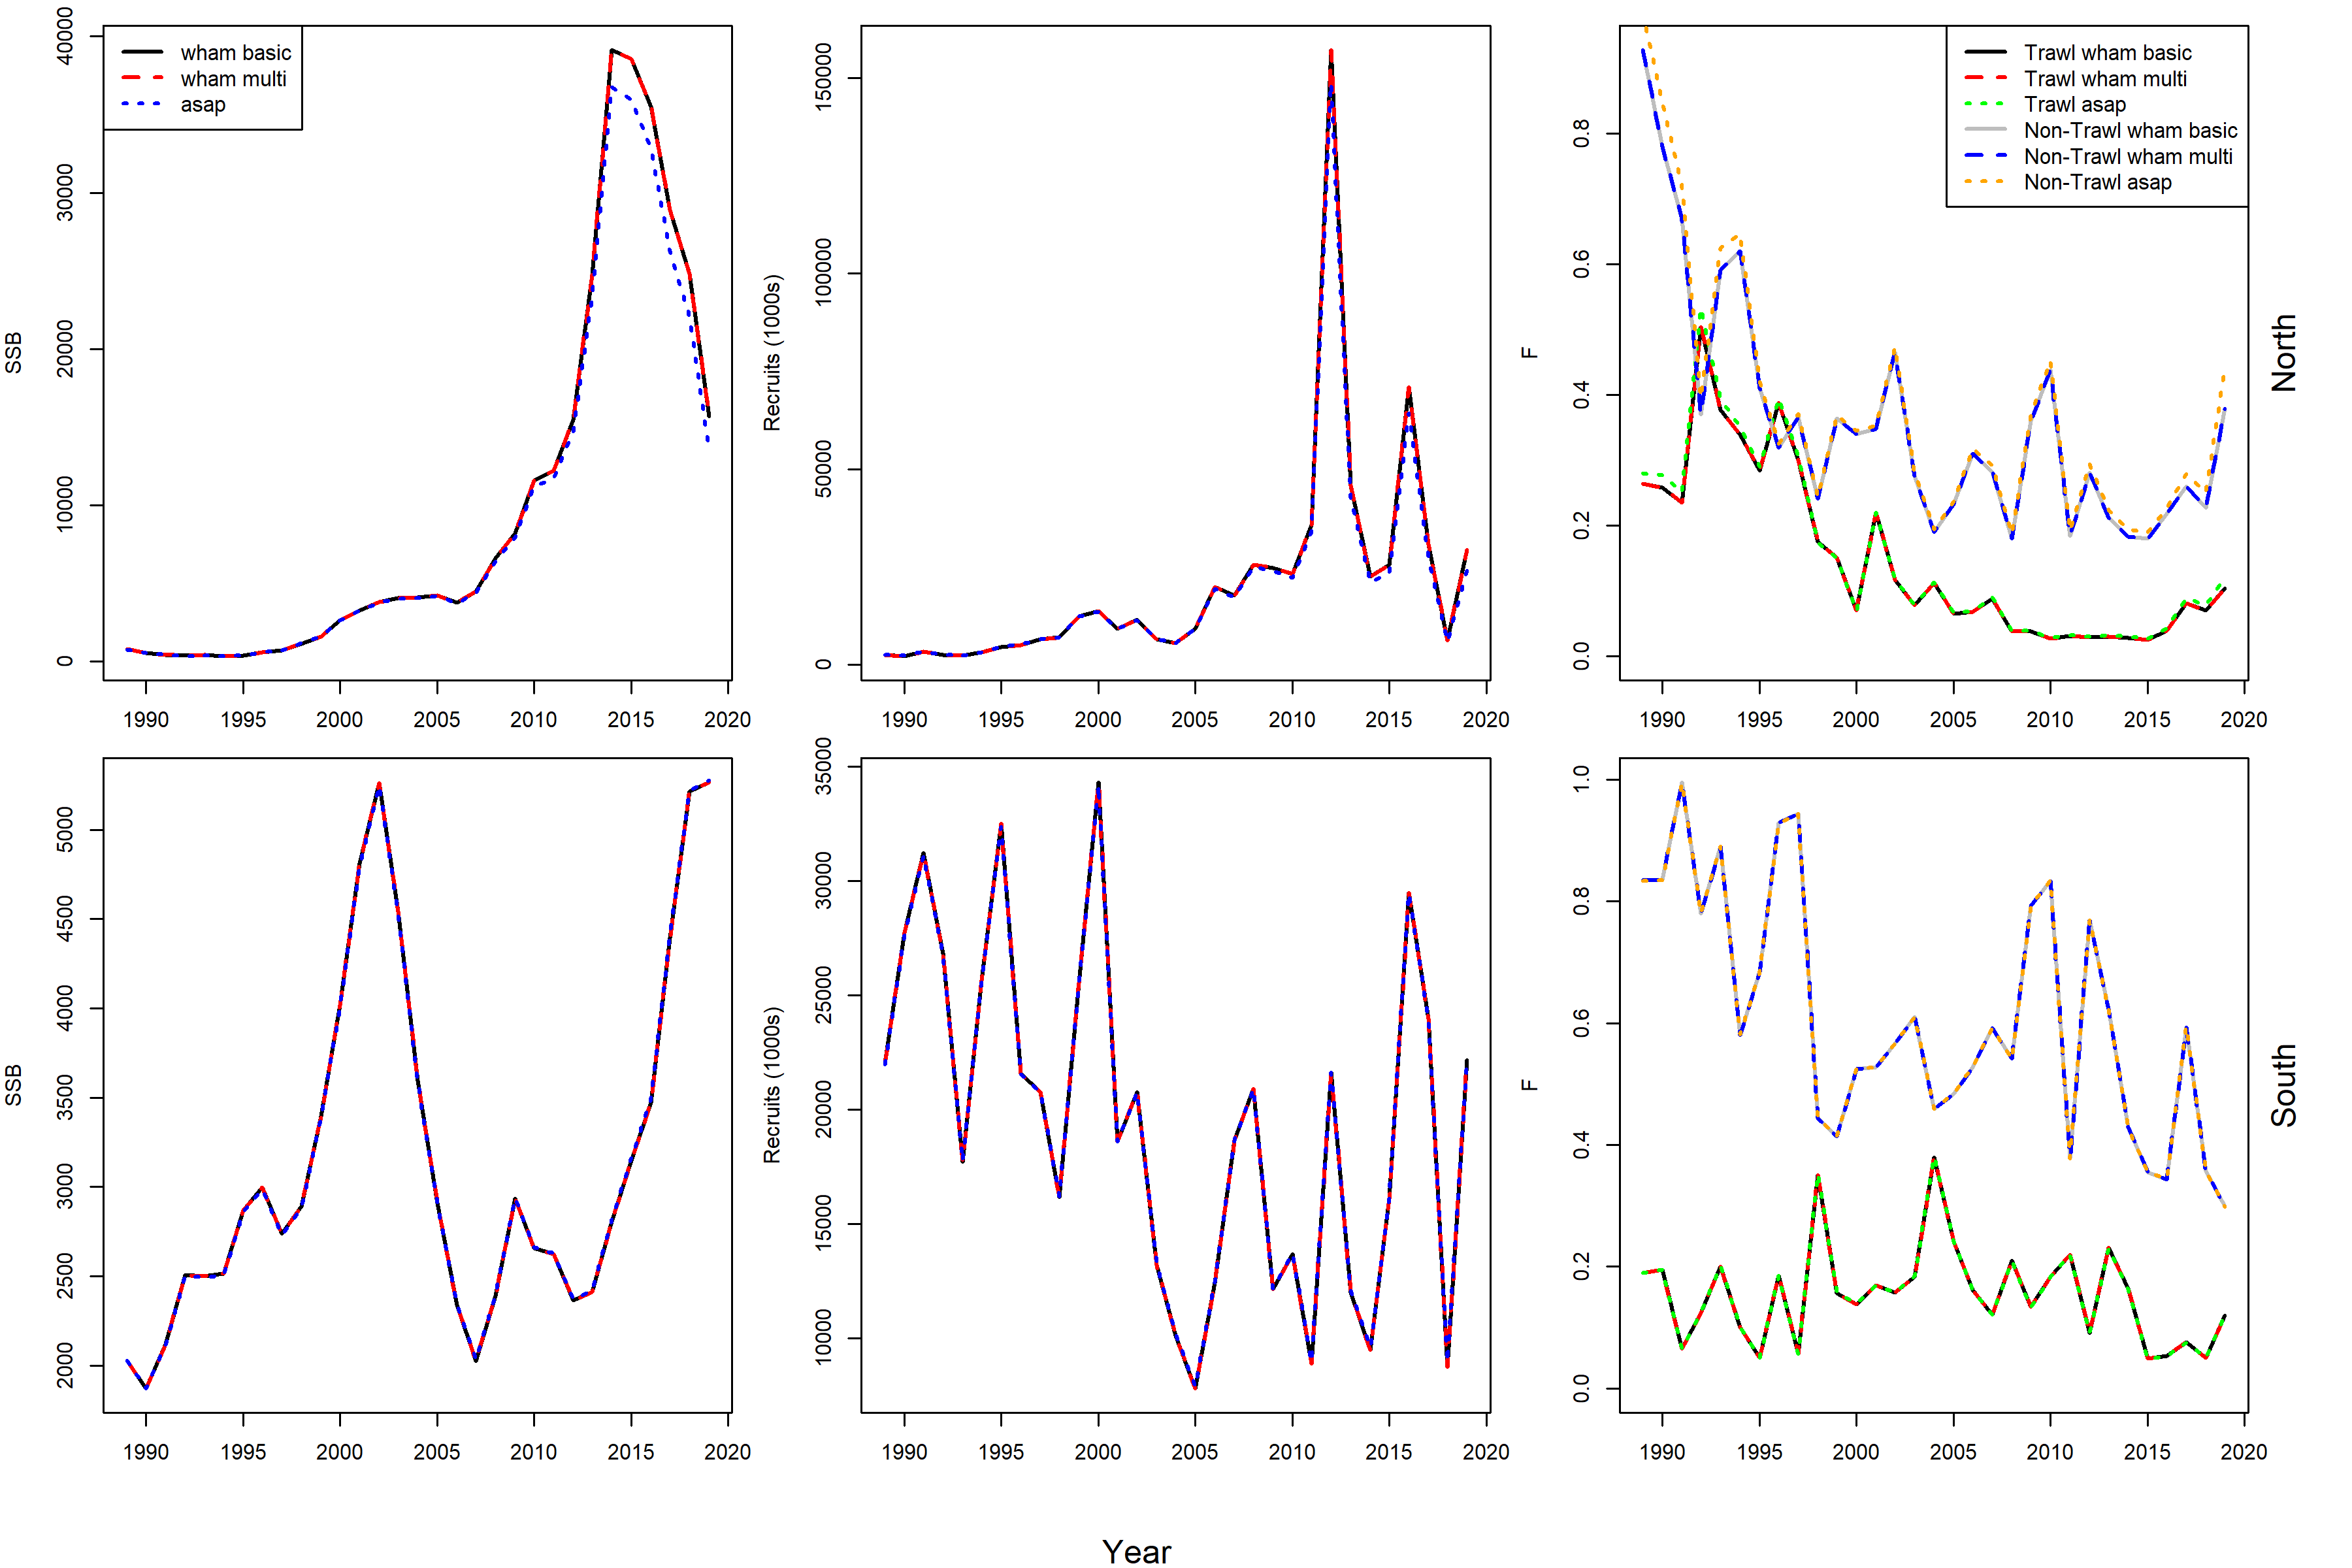
\includegraphics[width=0.75\linewidth]{plots/compare_one_stock_models} 

}

\caption{Comparison of recruitment, spawning stock biomass, and fishing mortality estimates from fitted models in ASAP3, the basic version of WHAM, and the multi-stock extension of WHAM to each regional component, separately, using ASAP3 model input files from the most recent management track assessment.}\label{fig:compare-asap-wham}
\end{figure}

\begin{figure}

{\centering 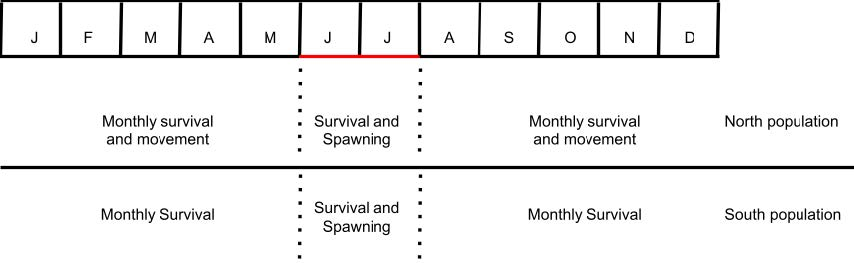
\includegraphics[width=0.8\linewidth]{plots/migration_diagram_1} 

}

\caption{Diagram of intervals within the year and configuation of the dynamics of each component of the BSB population.}\label{fig:unnamed-chunk-2}
\end{figure}
\elandscape

\begin{figure}

{\centering 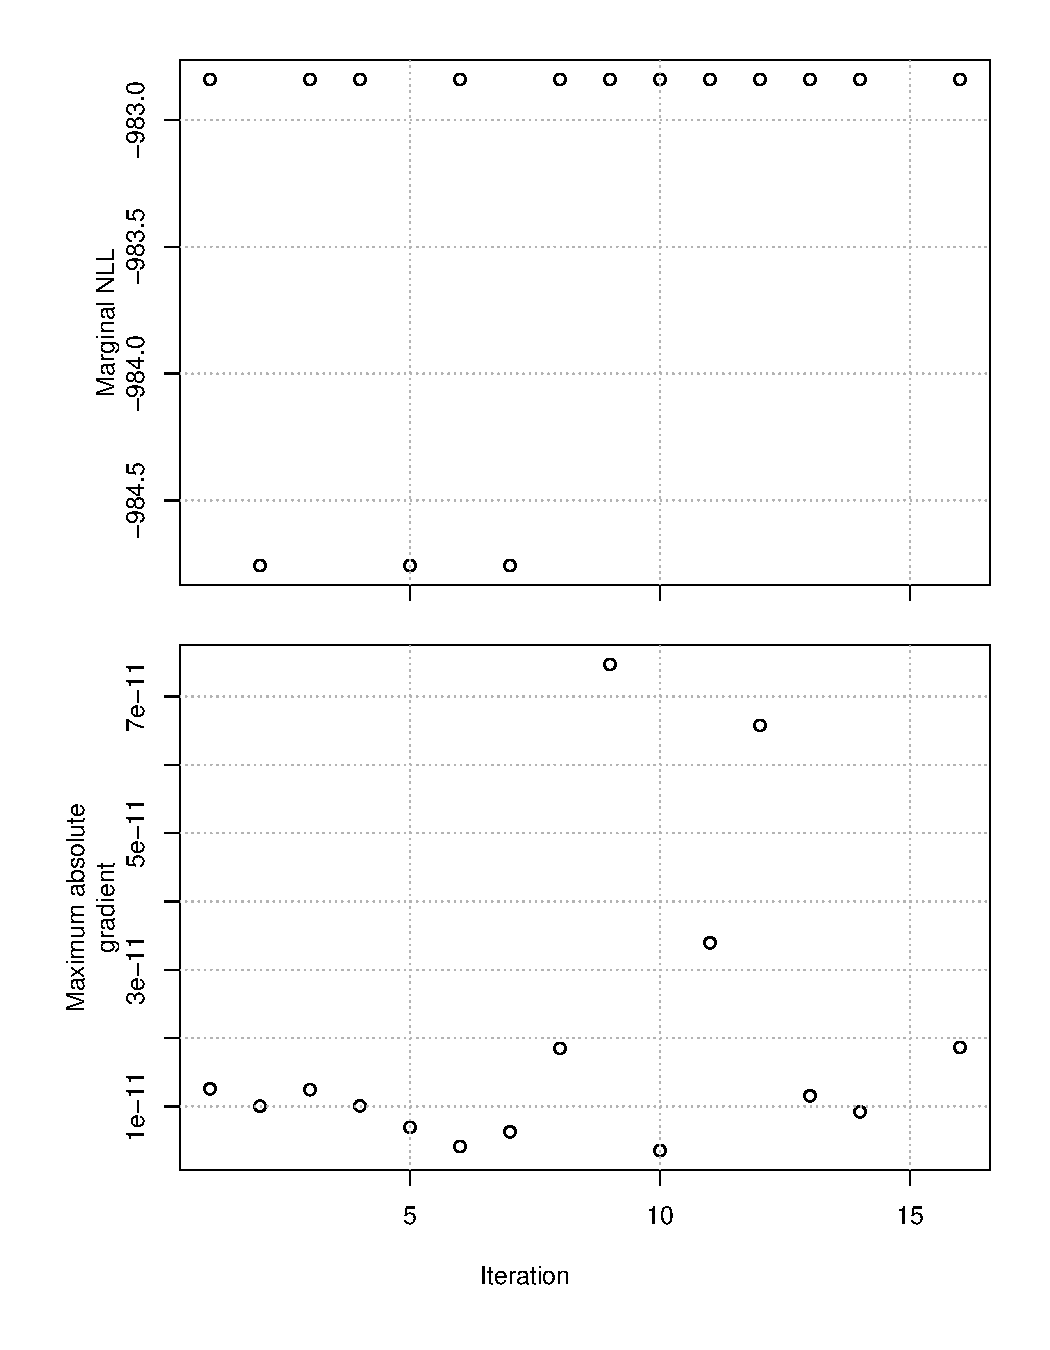
\includegraphics{bsb_models_wp_files/figure-latex/jitter-res-1-1} 

}

\caption{Marginal negative log-likelihood and maximum absolute value of gradients for each of 16 jitter iterations.}\label{fig:jitter-res-1}
\end{figure}
\clearpage

\begin{figure}

{\centering 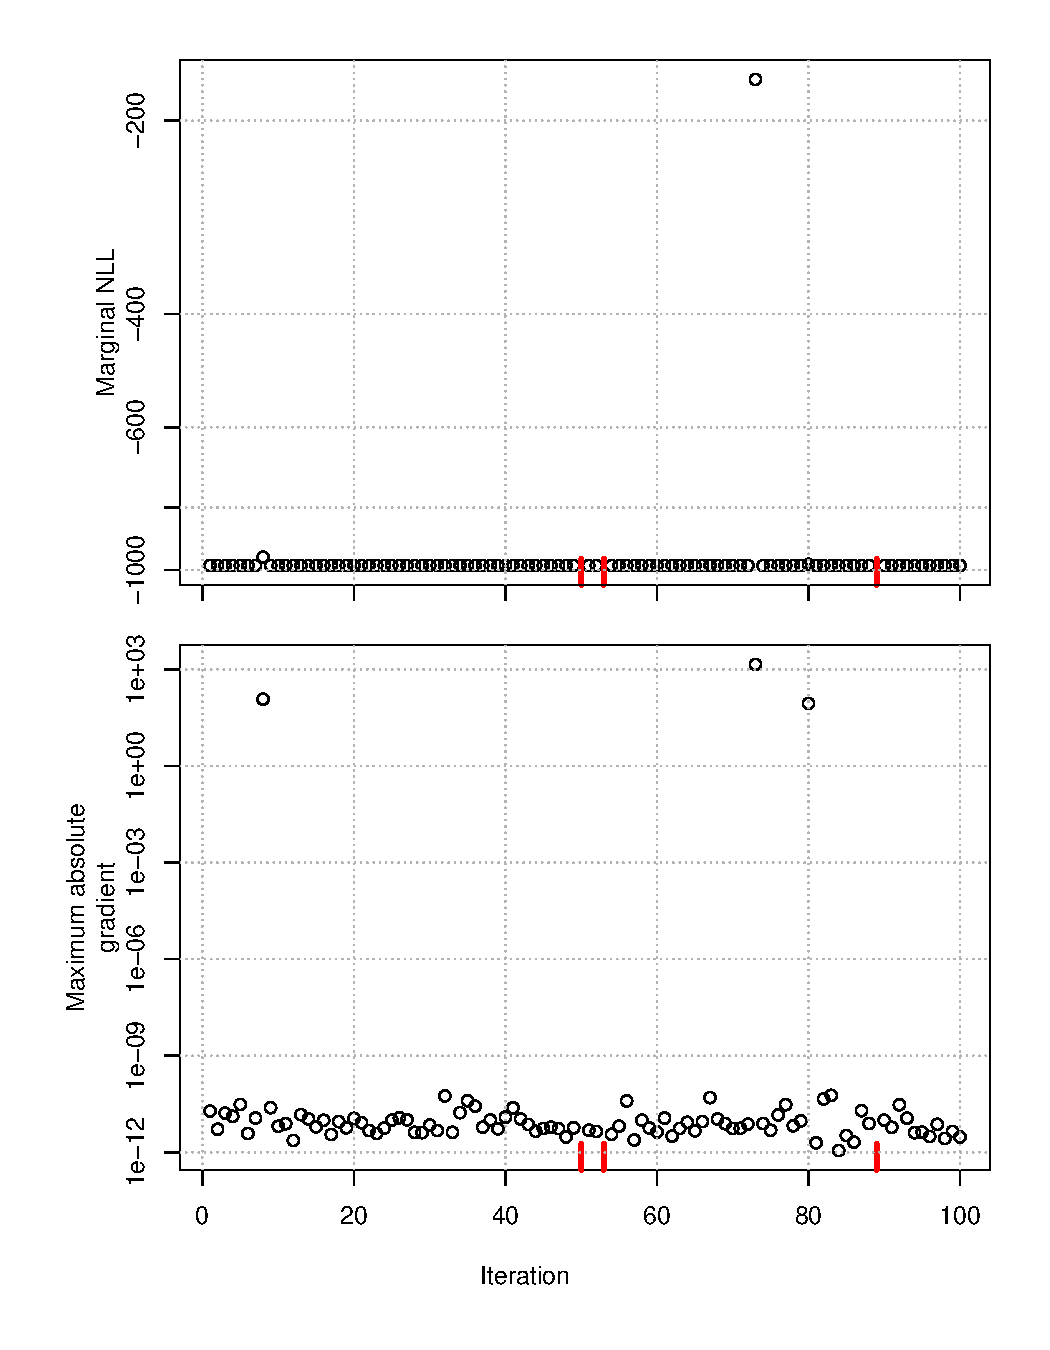
\includegraphics{bsb_models_wp_files/figure-latex/jitter-res-2-1} 

}

\caption{Marginal negative log-likelihood and maximum absolute value of gradients for each of 100 jitter iterations from revised Run 34 fit. Red rug lines indicate fits that failed to complete.}\label{fig:jitter-res-2}
\end{figure}

\begin{figure}

{\centering 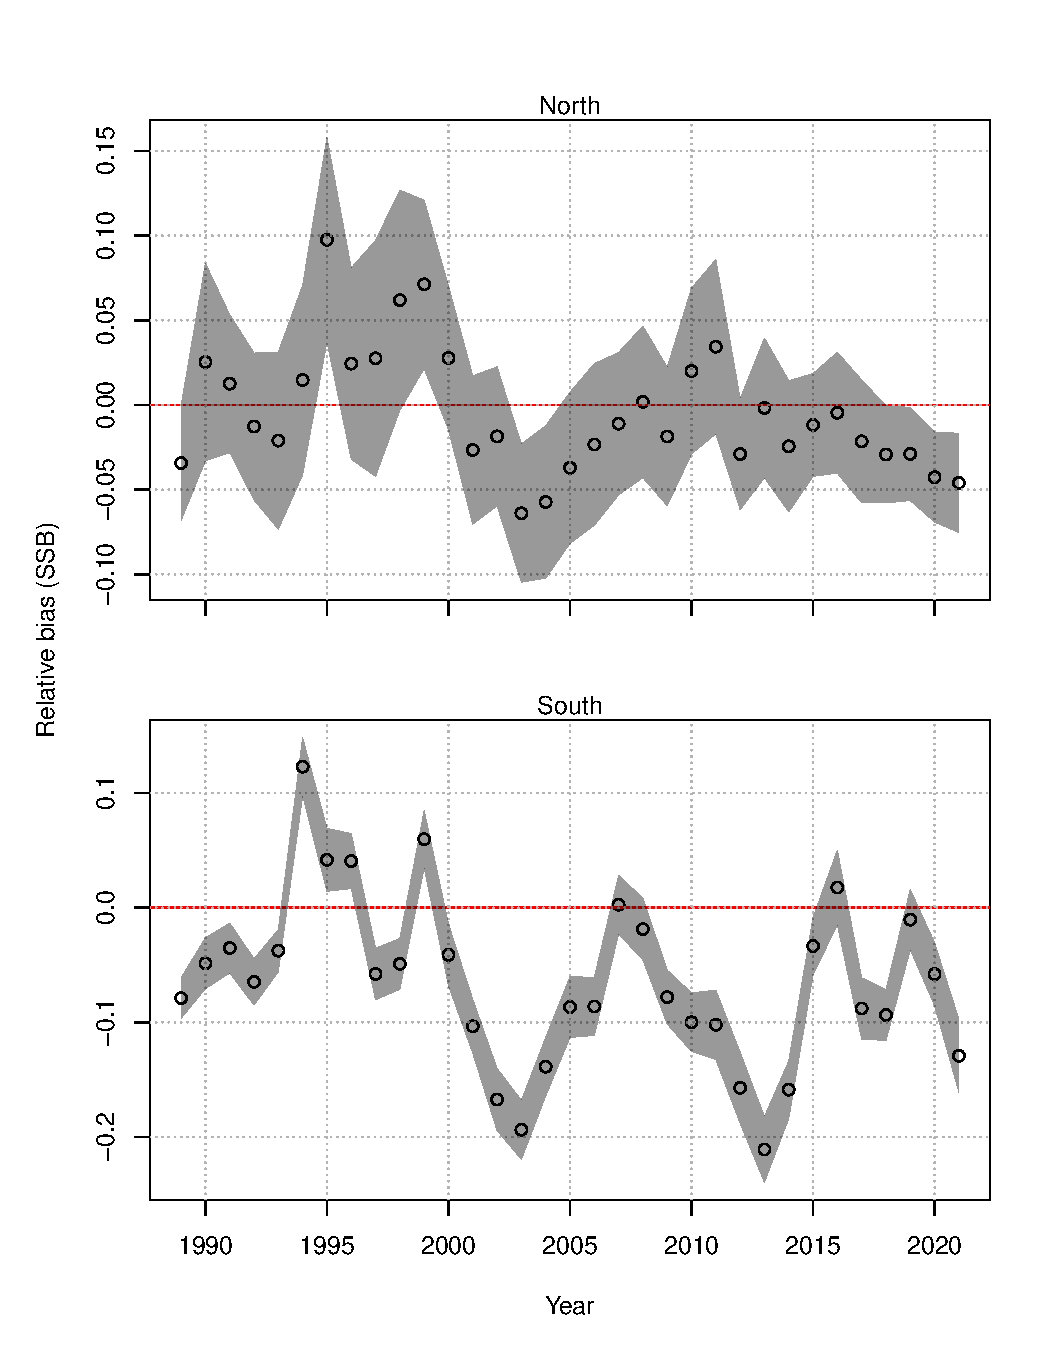
\includegraphics{bsb_models_wp_files/figure-latex/self-test-res-2-1} 

}

\caption{Relative bias of SSB estimates from conditional self test simulations.}\label{fig:self-test-res-2}
\end{figure}

\begin{figure}

{\centering 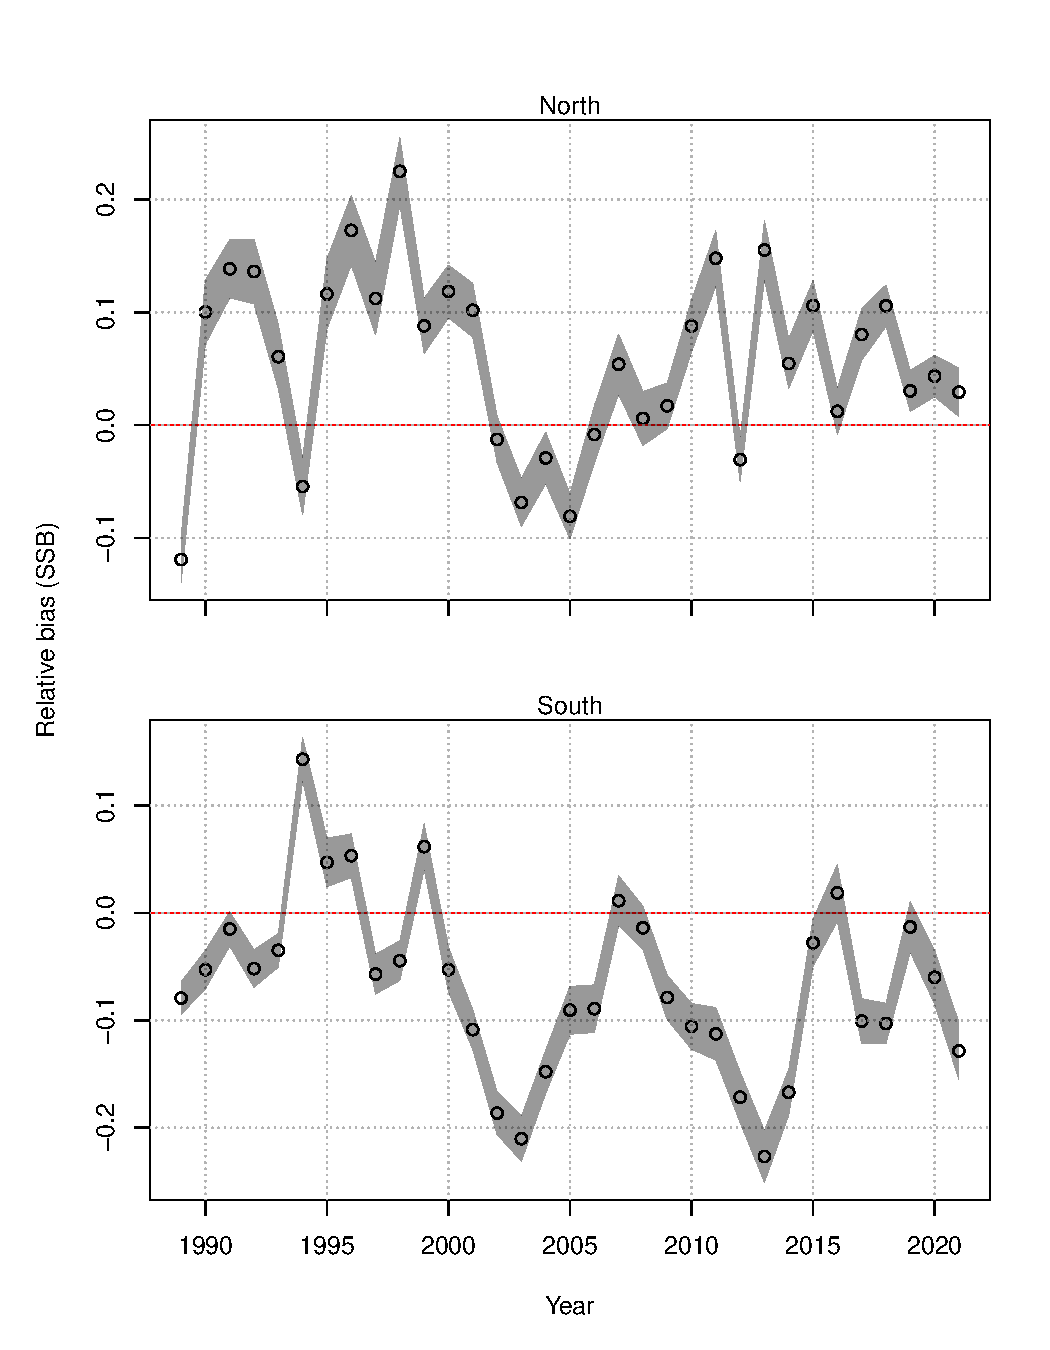
\includegraphics{bsb_models_wp_files/figure-latex/self-test-res-3-1} 

}

\caption{Relative bias of SSB estimates from conditional self test simulations with Rec CPA uncertainty scalar fixed at estimated values.}\label{fig:self-test-res-3}
\end{figure}

\begin{figure}

{\centering 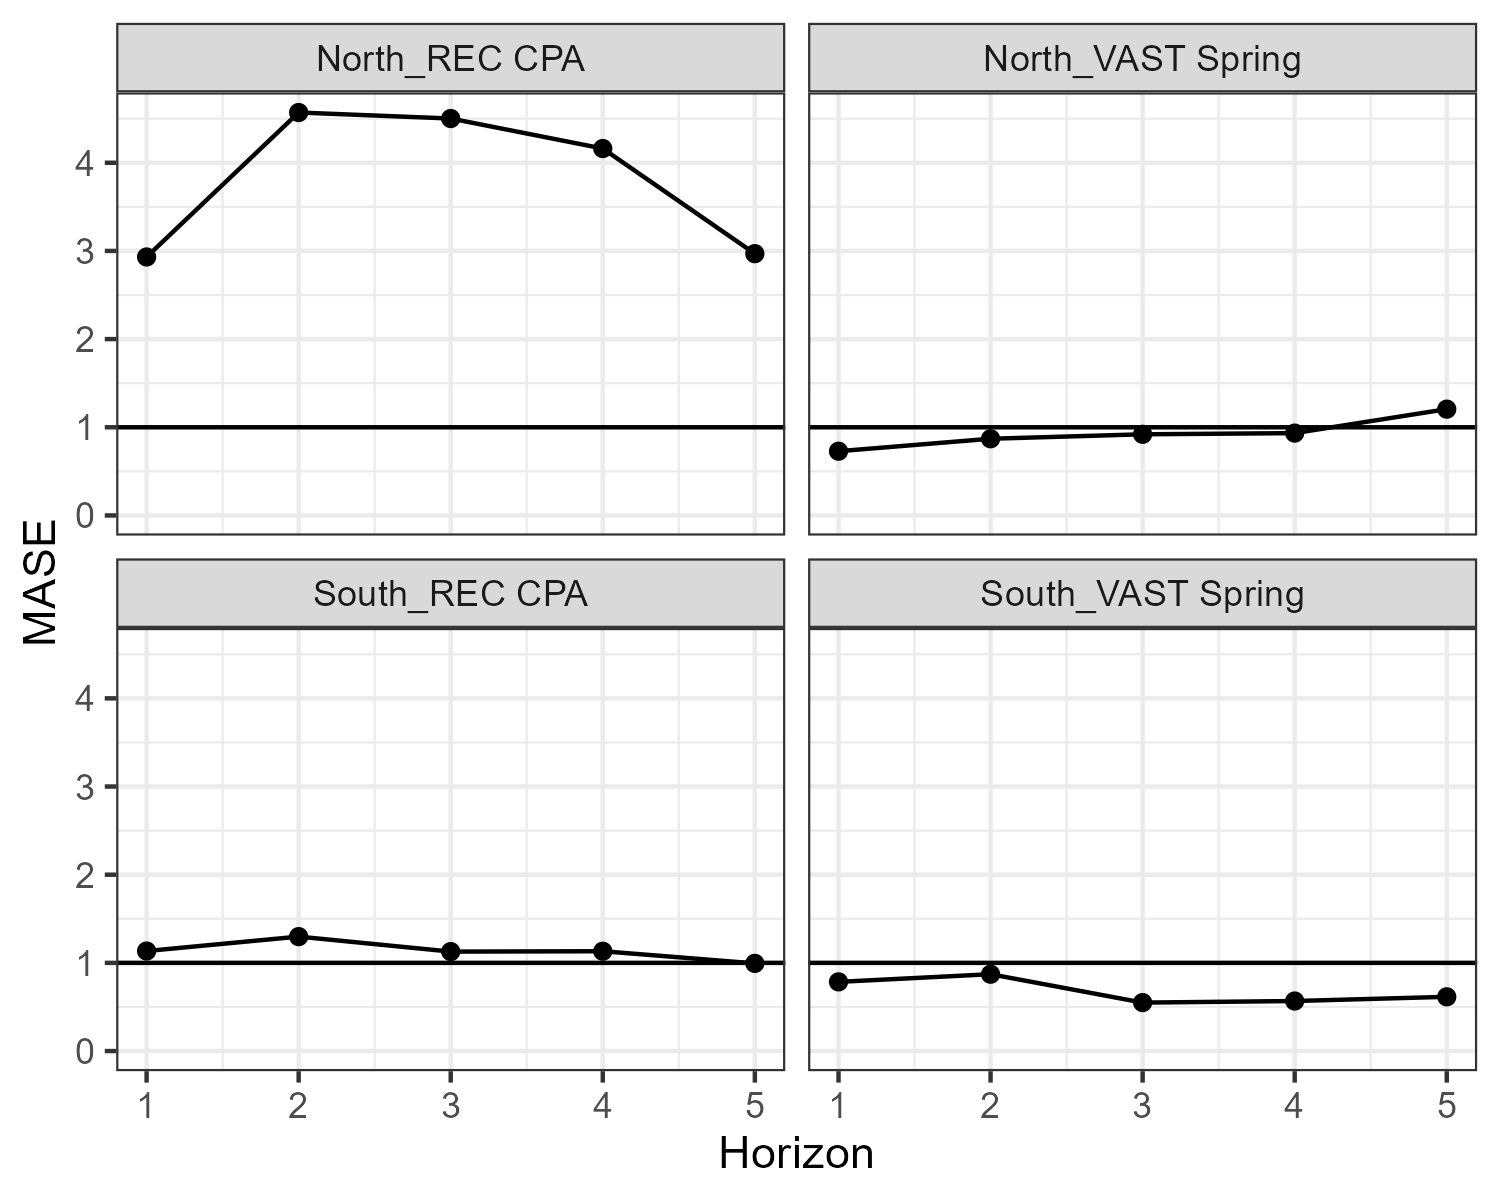
\includegraphics[width=1\linewidth]{../2023.RT.Runs/Run34/mase_WHAM for unnamed stock} 

}

\caption{MASE statistics for each index at alternative prediction horizons.}\label{fig:mase-by-index}
\end{figure}

\begin{figure}

{\centering 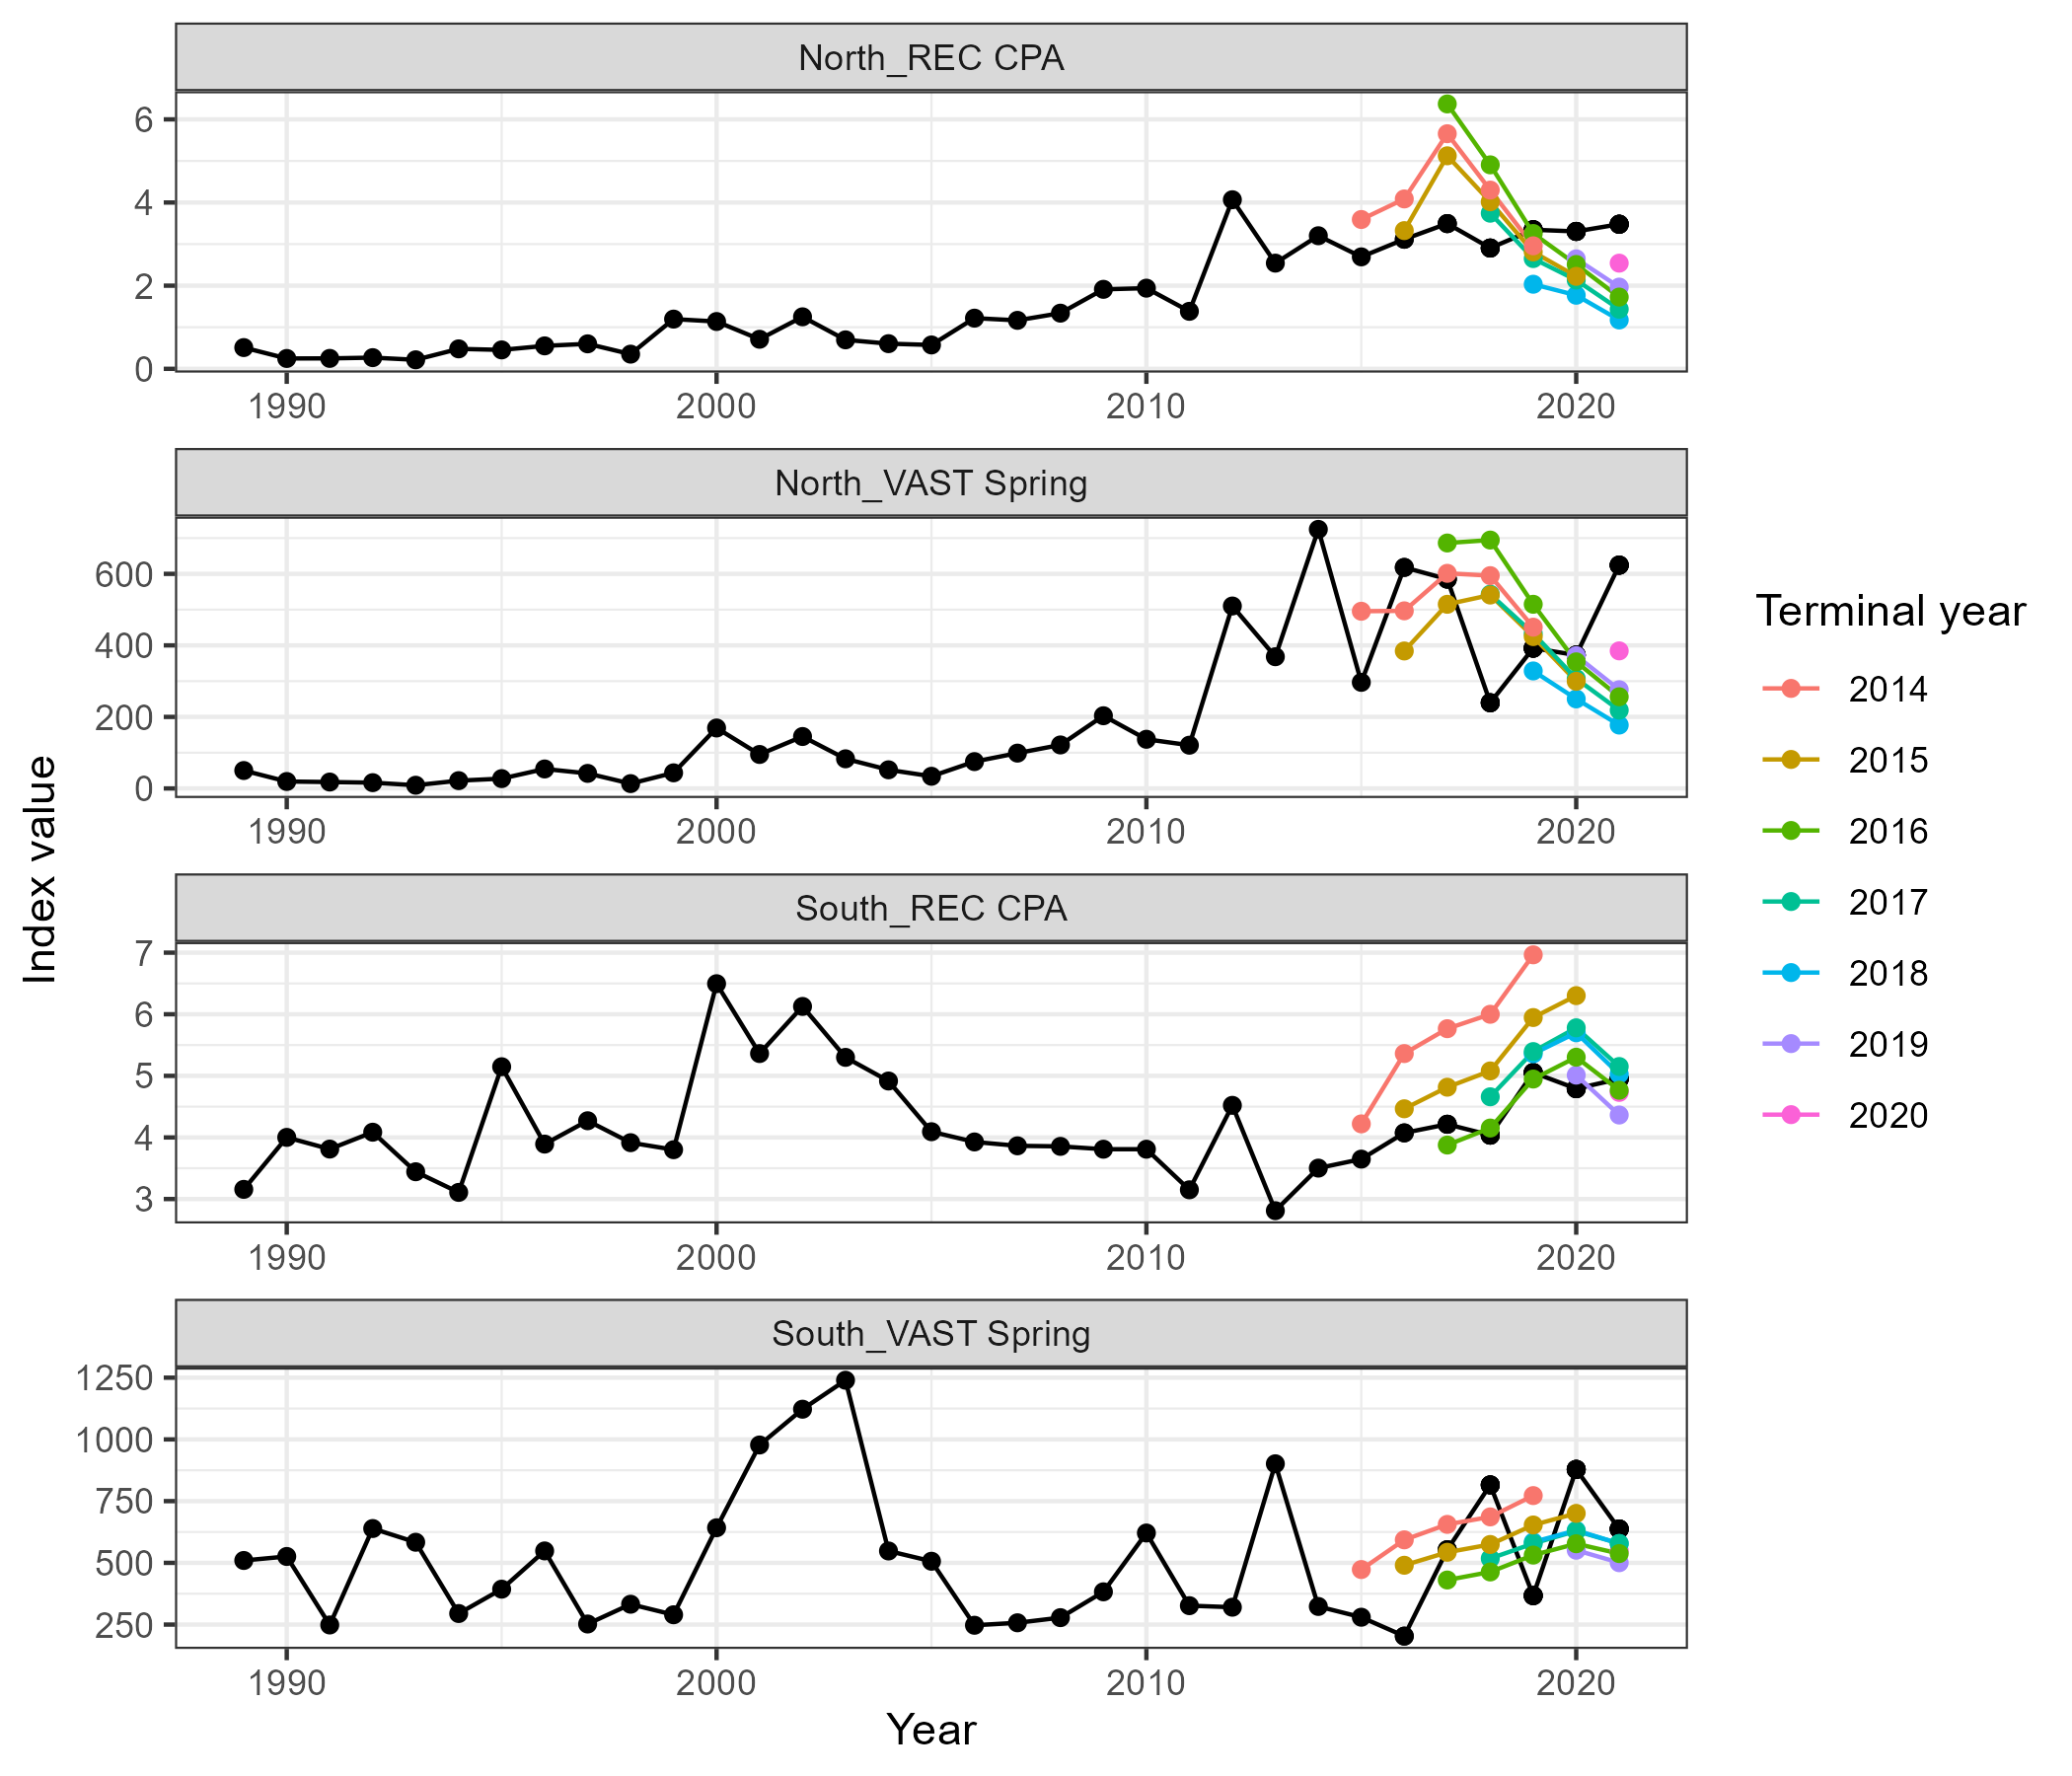
\includegraphics[width=1\linewidth]{../2023.RT.Runs/Run34/predicted_vs_obs_WHAM for unnamed stock} 

}

\caption{Index observations (black) and predictions for each MASE peel with all index and age composition observations removed.}\label{fig:mase-obs-pred-by-index}
\end{figure}

\begin{figure}

{\centering 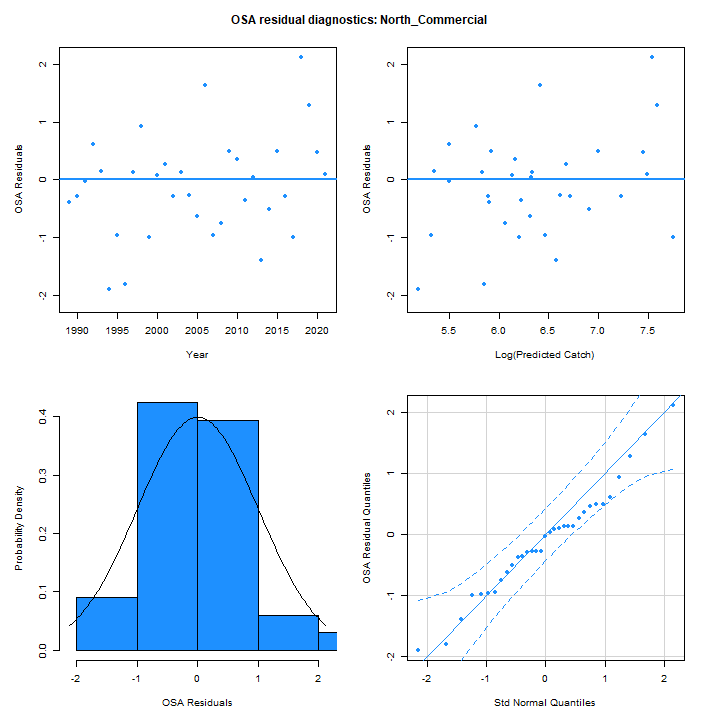
\includegraphics[width=1\linewidth]{../2023.RT.Runs/Run34/plots_png/diagnostics/OSA_resid_catch_4panel_North_Commercial} 

}

\caption{Summary plots for aggregate catch one-step-ahead residuals for the Northern commercial fleet.}\label{fig:osa-North-comm-catch-summ}
\end{figure}
\begin{figure}

{\centering 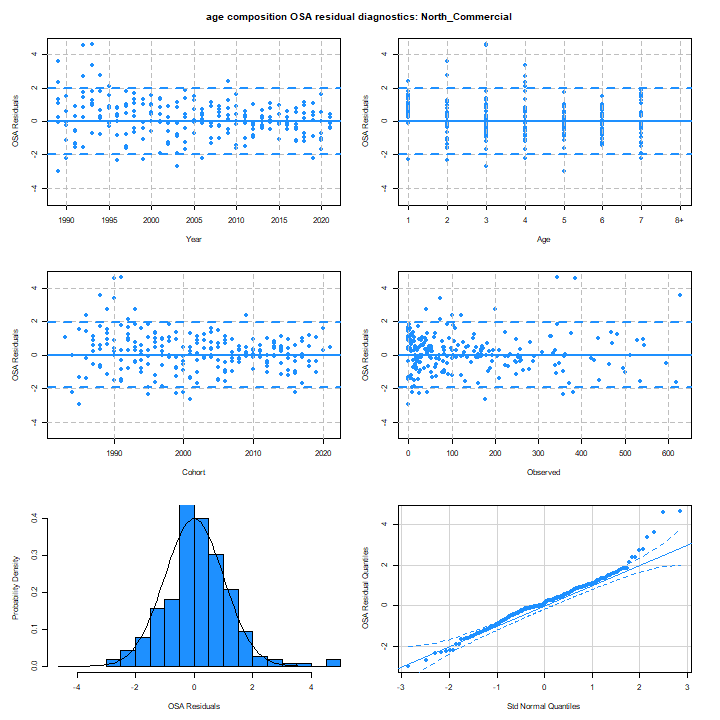
\includegraphics[width=1\linewidth]{../2023.RT.Runs/Run34/plots_png/diagnostics/OSA_resid_paa_6panel_North_Commercial} 

}

\caption{Summary plots for age composition one-step-ahead residuals for the Northern commercial fleet.}\label{fig:osa-North-comm-paa-summ}
\end{figure}
\begin{figure}

{\centering 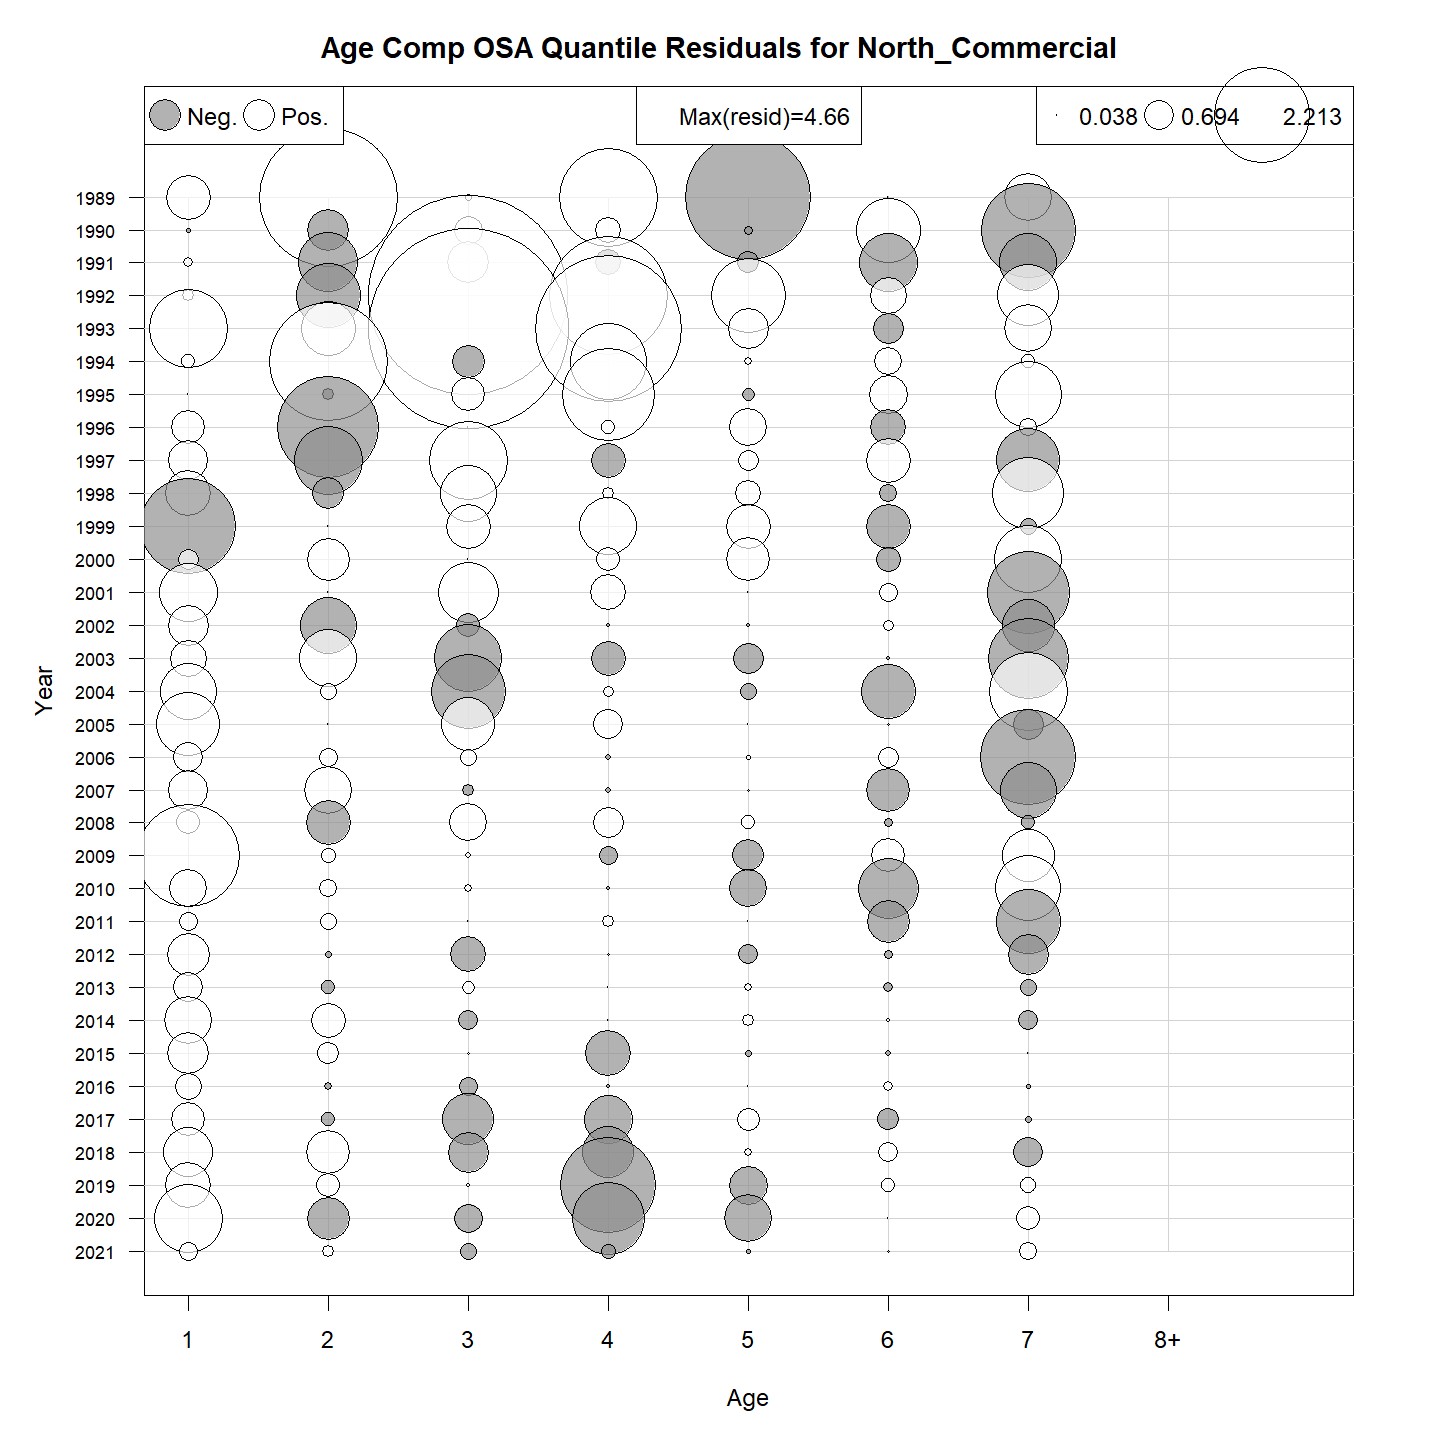
\includegraphics[width=1\linewidth]{../2023.RT.Runs/Run34/plots_png/diagnostics/Catch_age_comp_osa_resids_North_Commercial} 

}

\caption{One-step-ahead residuals for age composition of the Northern commercial fleet.}\label{fig:osa-North-comm-paa}
\end{figure}

\begin{figure}

{\centering 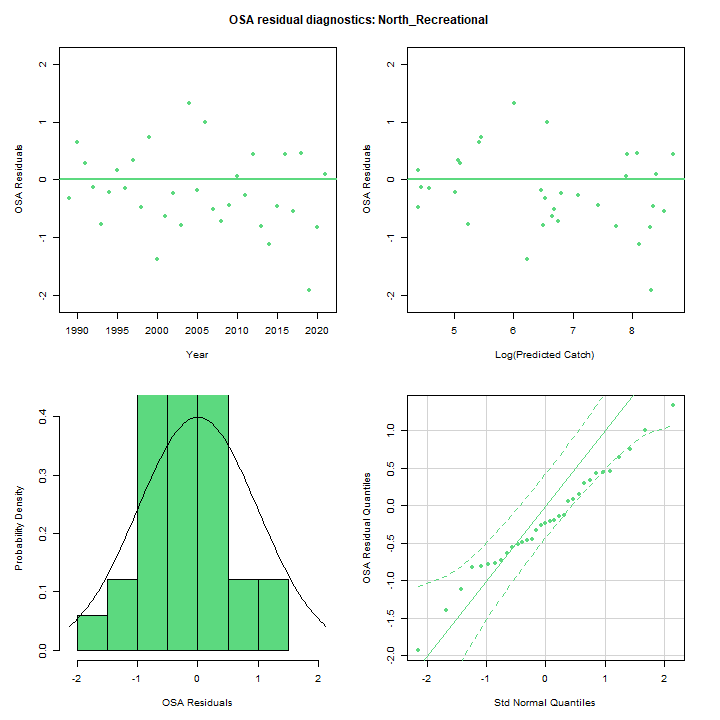
\includegraphics[width=1\linewidth]{../2023.RT.Runs/Run34/plots_png/diagnostics/OSA_resid_catch_4panel_North_Recreational} 

}

\caption{Summary plots for aggregate catch one-step-ahead residuals for the Northern recreational fleet.}\label{fig:osa-North-rec-catch-summ}
\end{figure}
\begin{figure}

{\centering 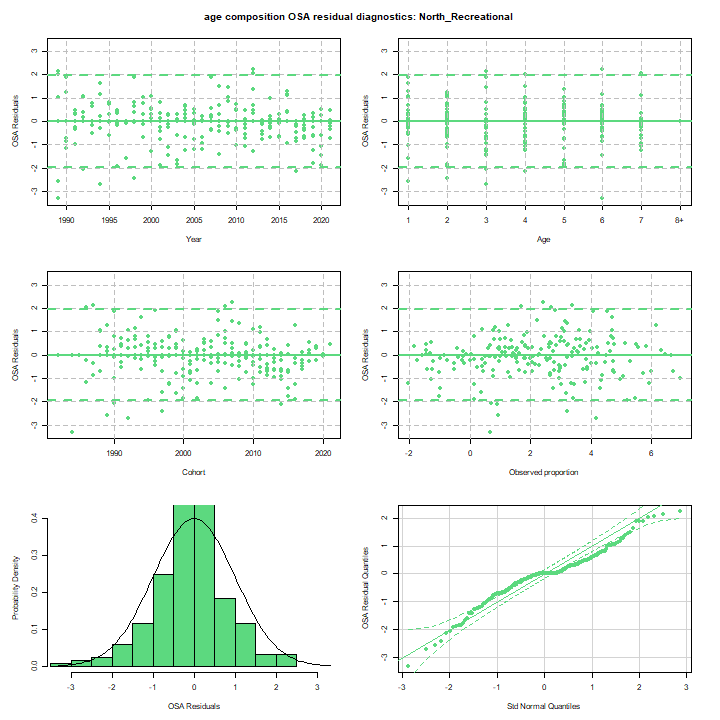
\includegraphics[width=1\linewidth]{../2023.RT.Runs/Run34/plots_png/diagnostics/OSA_resid_paa_6panel_North_Recreational} 

}

\caption{Summary plots for age composition one-step-ahead residuals for the Northern recreational fleet.}\label{fig:osa-North-rec-paa-summ}
\end{figure}
\begin{figure}

{\centering 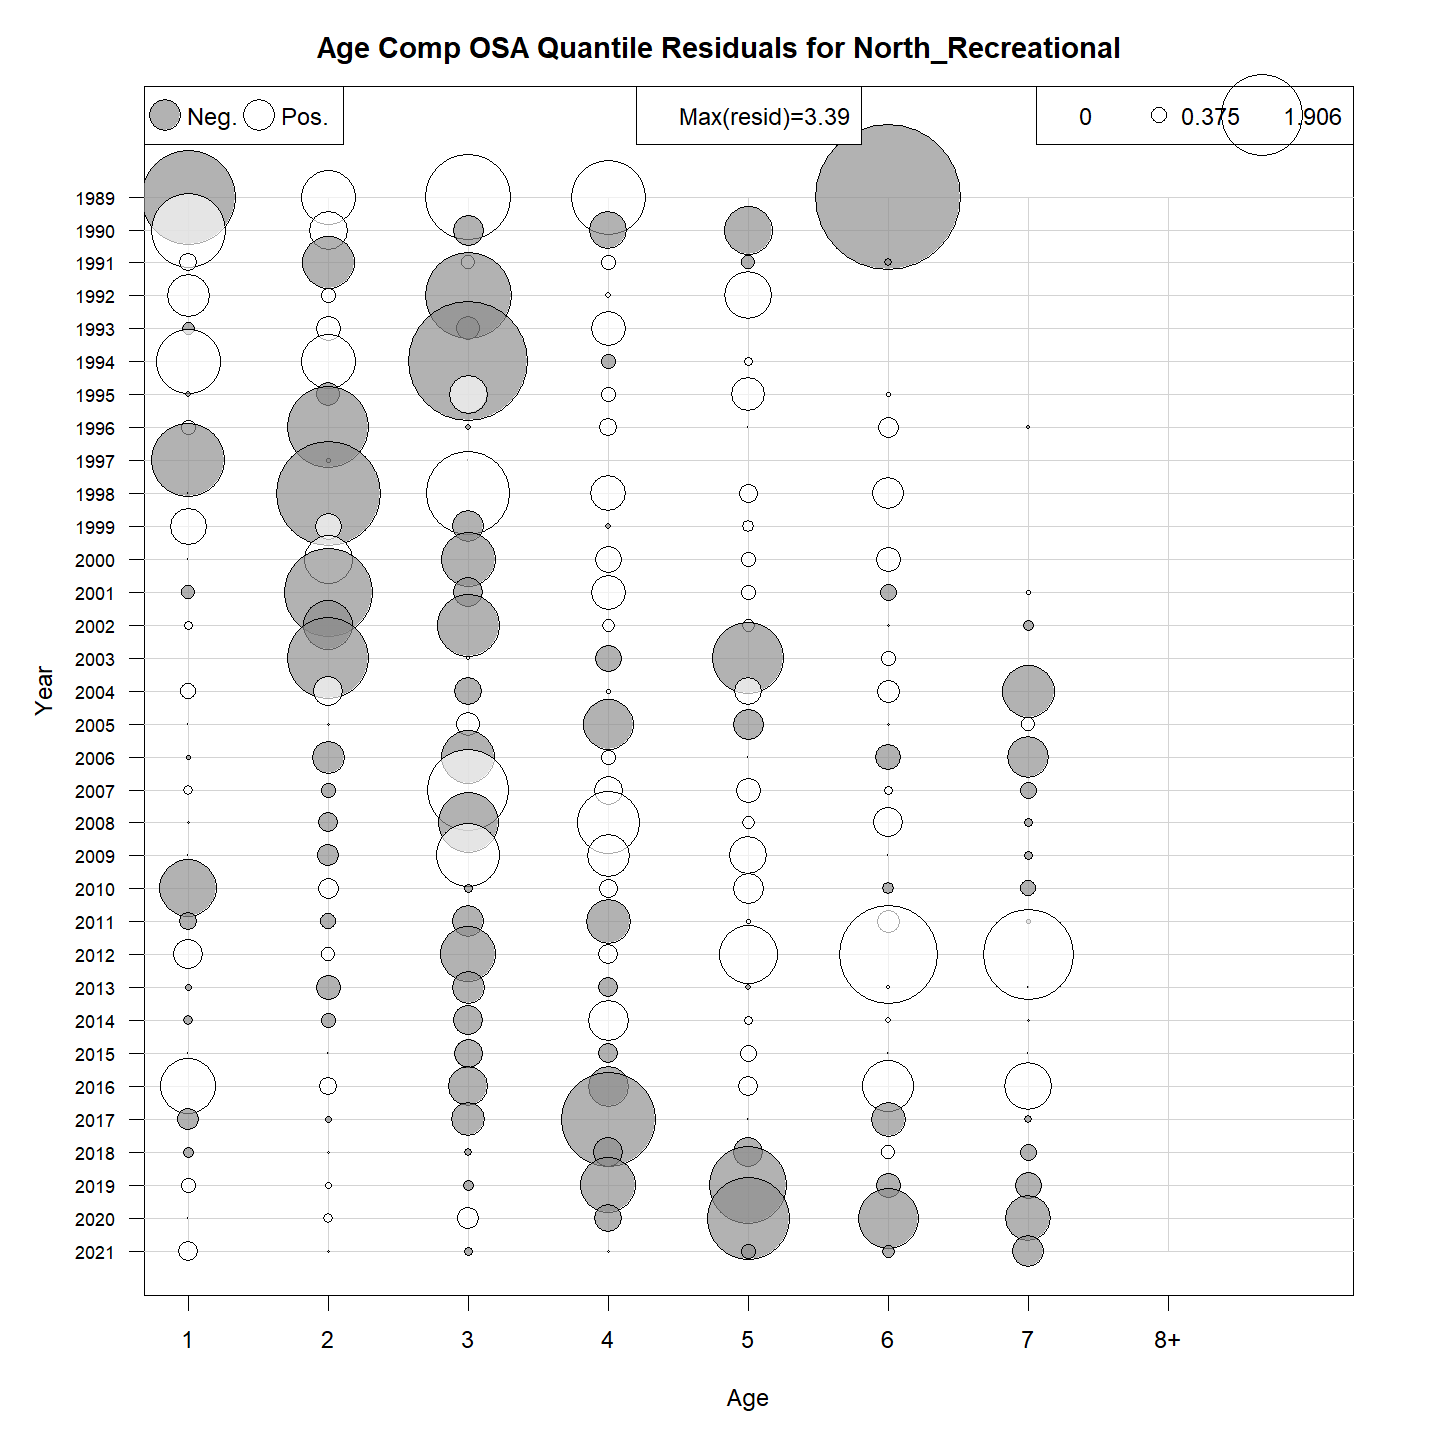
\includegraphics[width=1\linewidth]{../2023.RT.Runs/Run34/plots_png/diagnostics/Catch_age_comp_osa_resids_North_Recreational} 

}

\caption{One-step-ahead residuals for age composition of the Northern recreational fleet.}\label{fig:osa-North-rec-paa}
\end{figure}

\begin{figure}

{\centering 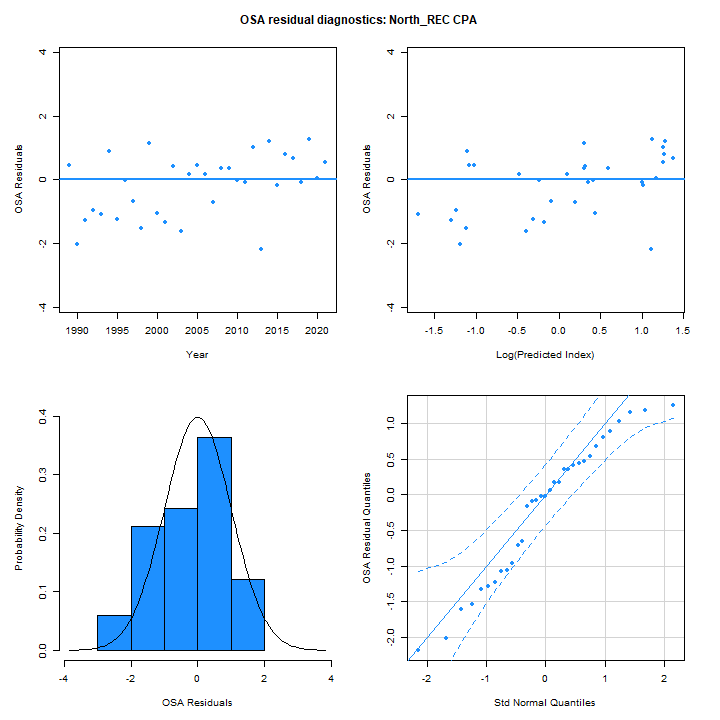
\includegraphics[width=1\linewidth]{../2023.RT.Runs/Run34/plots_png/diagnostics/OSA_resid_catch_4panel_North_REC_CPA} 

}

\caption{Summary plots for aggregate catch one-step-ahead residuals for the Northern Recreational CPA index.}\label{fig:osa-North-reccpa-catch-summ}
\end{figure}
\begin{figure}

{\centering 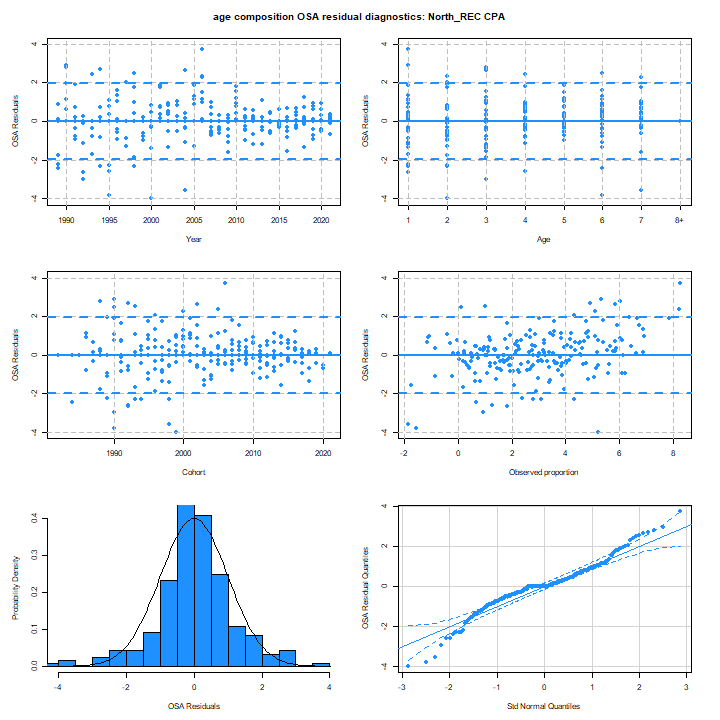
\includegraphics[width=1\linewidth]{../2023.RT.Runs/Run34/plots_png/diagnostics/OSA_resid_paa_6panel_North_REC_CPA} 

}

\caption{Summary plots for age composition one-step-ahead residuals for the Northern Recreational CPA index.}\label{fig:osa-North-reccpa-paa-summ}
\end{figure}
\begin{figure}

{\centering 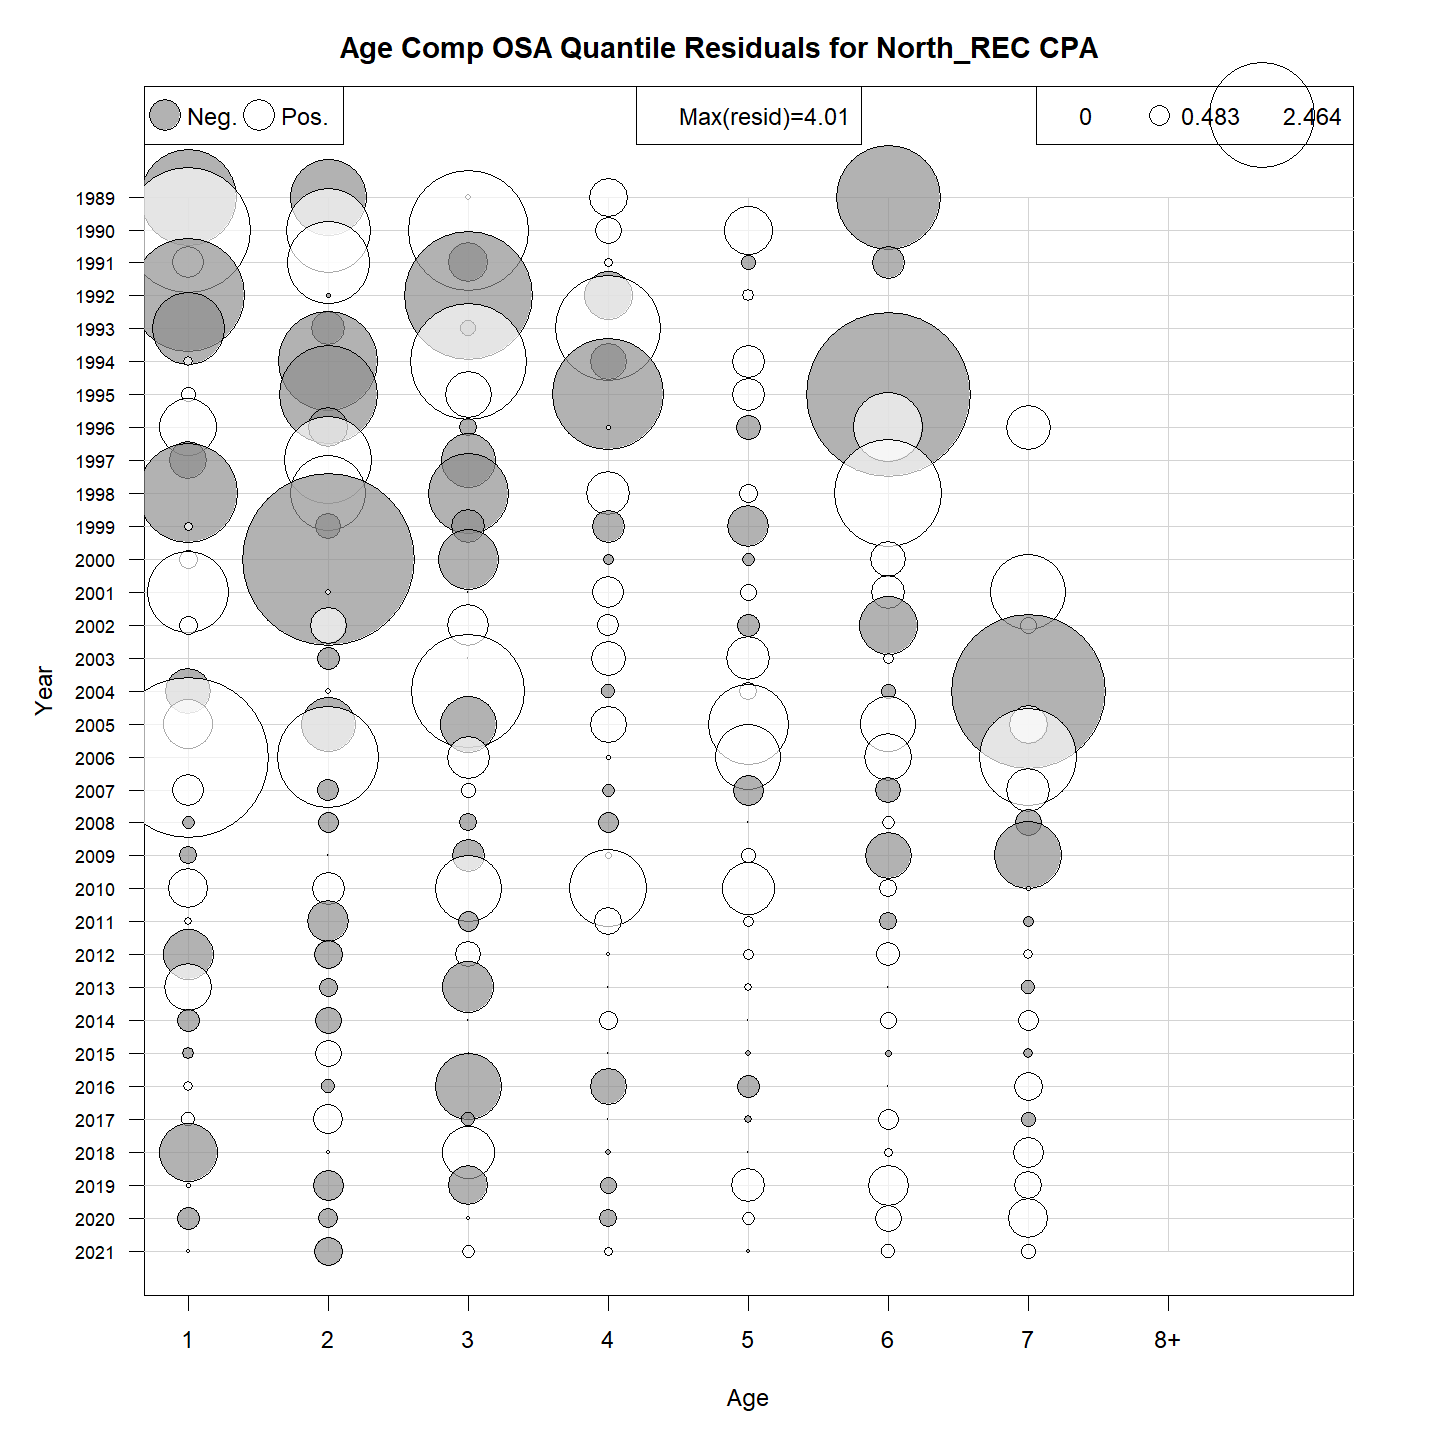
\includegraphics[width=1\linewidth]{../2023.RT.Runs/Run34/plots_png/diagnostics/Catch_age_comp_osa_resids_North_REC_CPA} 

}

\caption{One-step-ahead residuals for age composition of the Northern Recreational CPA index.}\label{fig:osa-North-reccpa-paa}
\end{figure}

\begin{figure}

{\centering 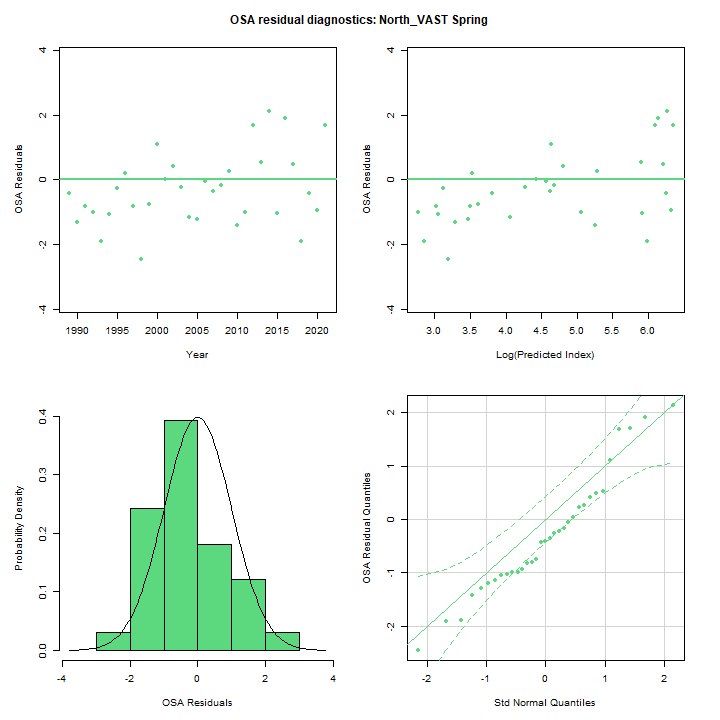
\includegraphics[width=1\linewidth]{../2023.RT.Runs/Run34/plots_png/diagnostics/OSA_resid_catch_4panel_North_VAST_Spring} 

}

\caption{Summary plots for aggregate catch one-step-ahead residuals for the Northern VAST index.}\label{fig:osa-North-vast-catch-summ}
\end{figure}
\begin{figure}

{\centering 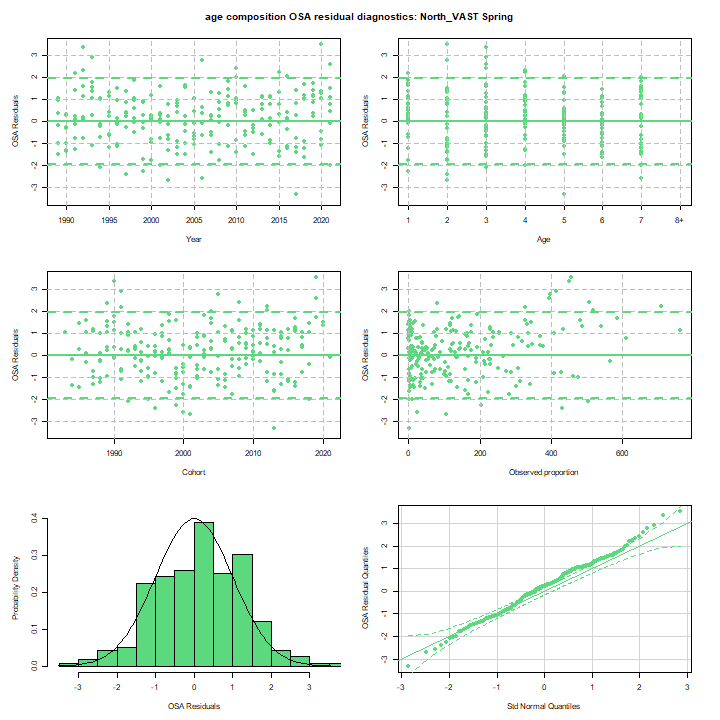
\includegraphics[width=1\linewidth]{../2023.RT.Runs/Run34/plots_png/diagnostics/OSA_resid_paa_6panel_North_VAST_Spring} 

}

\caption{Summary plots for age composition one-step-ahead residuals for the Northern VAST index.}\label{fig:osa-North-vast-paa-summ}
\end{figure}
\begin{figure}

{\centering 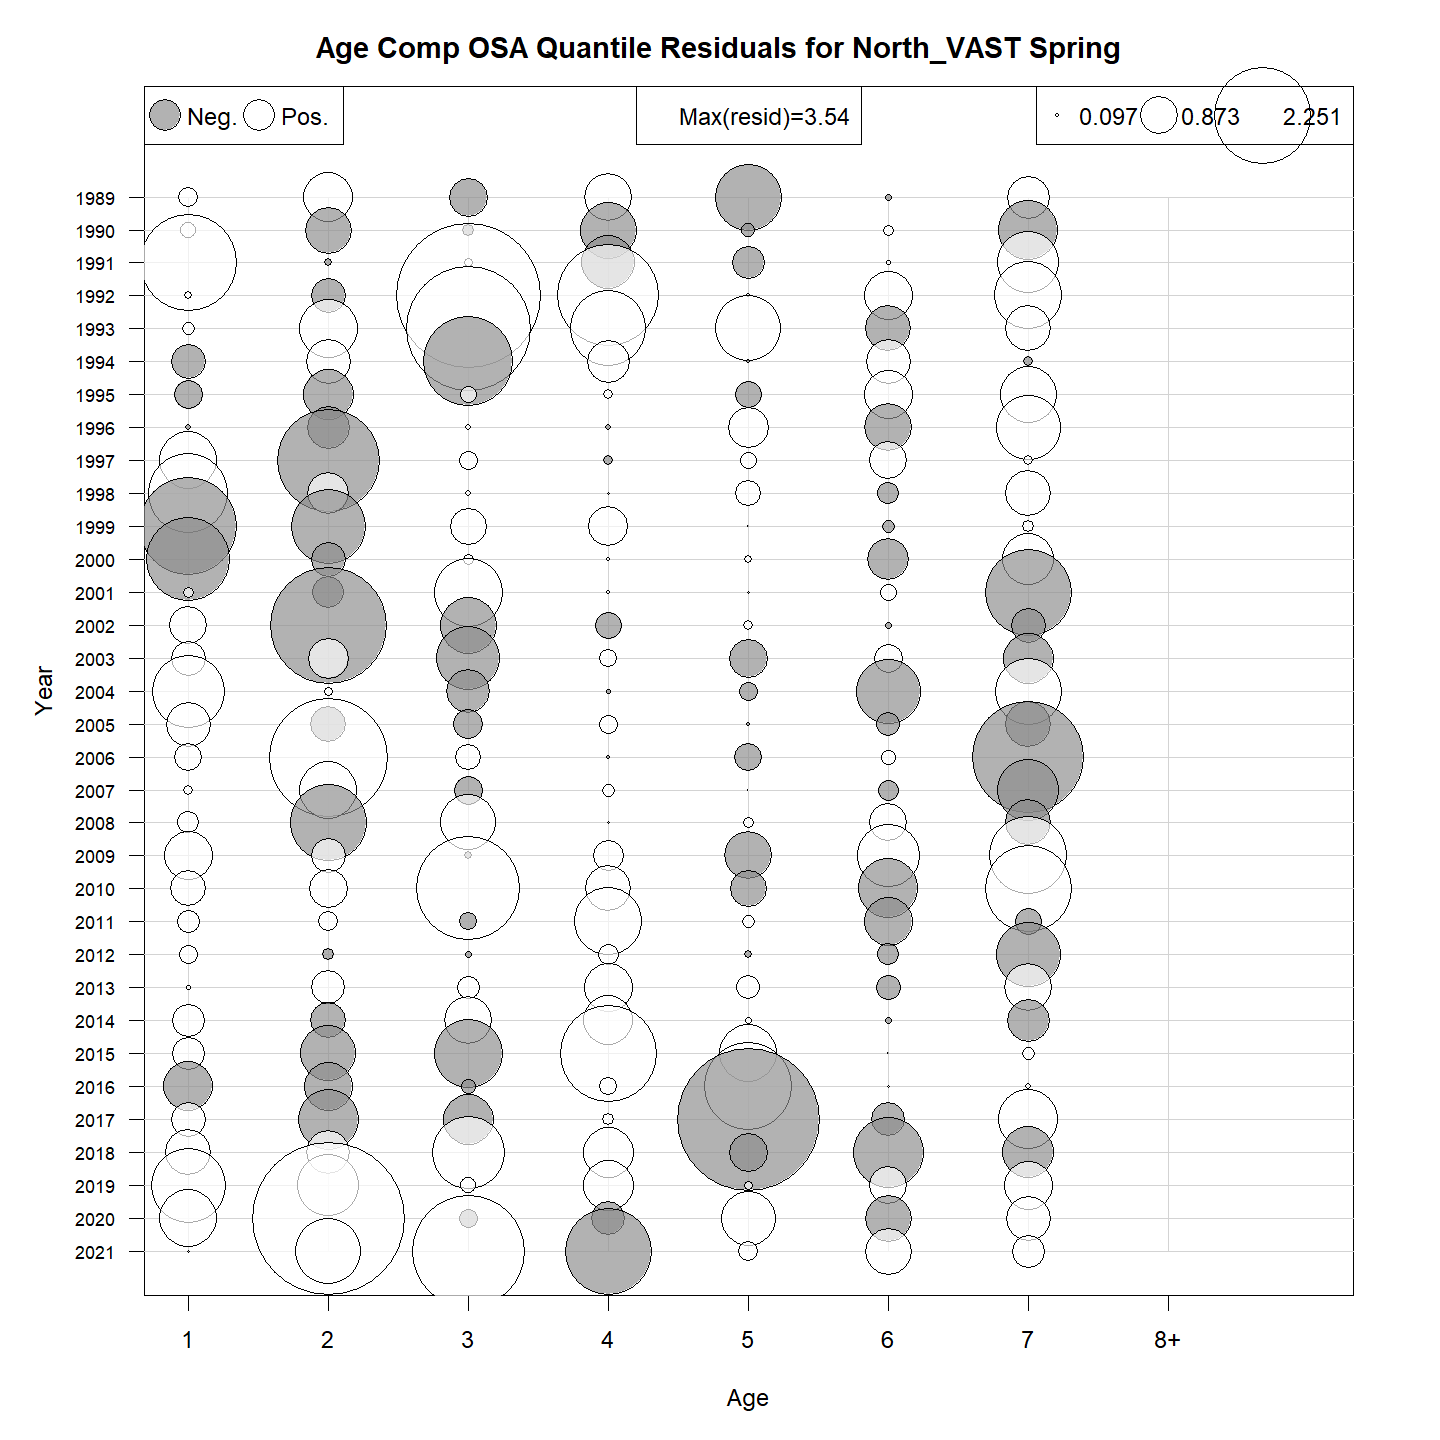
\includegraphics[width=1\linewidth]{../2023.RT.Runs/Run34/plots_png/diagnostics/Catch_age_comp_osa_resids_North_VAST_Spring} 

}

\caption{One-step-ahead residuals for age composition of the Northern VAST index.}\label{fig:osa-North-vast-paa}
\end{figure}

\begin{figure}

{\centering 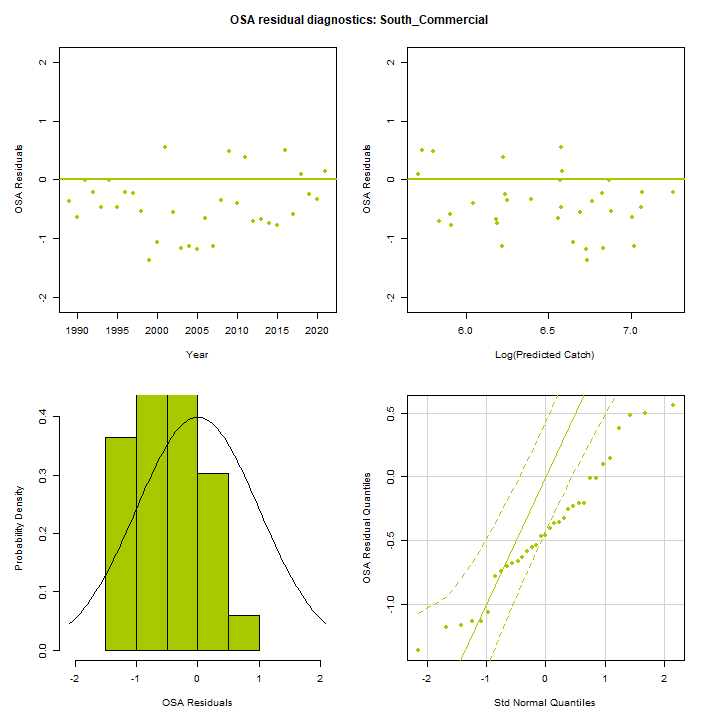
\includegraphics[width=1\linewidth]{../2023.RT.Runs/Run34/plots_png/diagnostics/OSA_resid_catch_4panel_South_Commercial} 

}

\caption{Summary plots for aggregate catch one-step-ahead residuals for the Southern commercial fleet.}\label{fig:osa-South-comm-catch-summ}
\end{figure}
\begin{figure}

{\centering 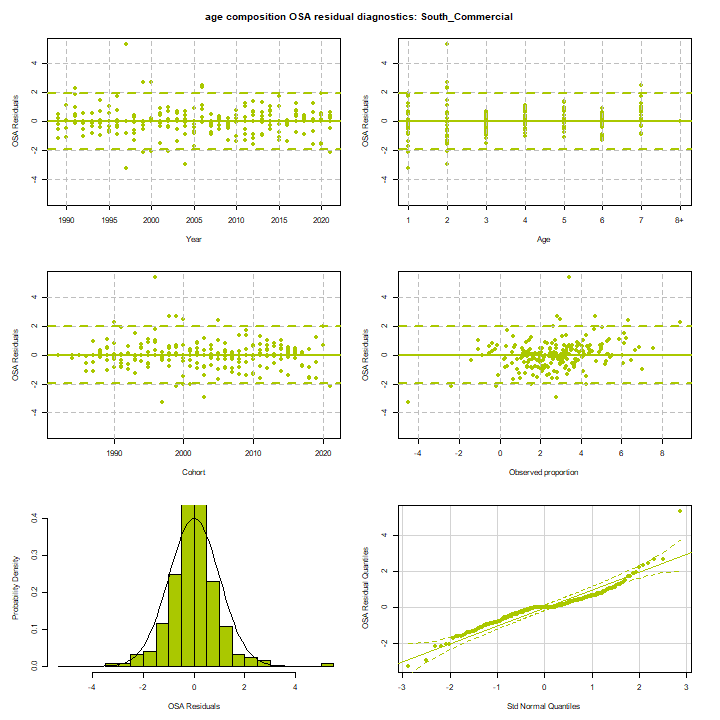
\includegraphics[width=1\linewidth]{../2023.RT.Runs/Run34/plots_png/diagnostics/OSA_resid_paa_6panel_South_Commercial} 

}

\caption{Summary plots for age composition one-step-ahead residuals for the Southern commercial fleet.}\label{fig:osa-South-comm-paa-summ}
\end{figure}
\begin{figure}

{\centering 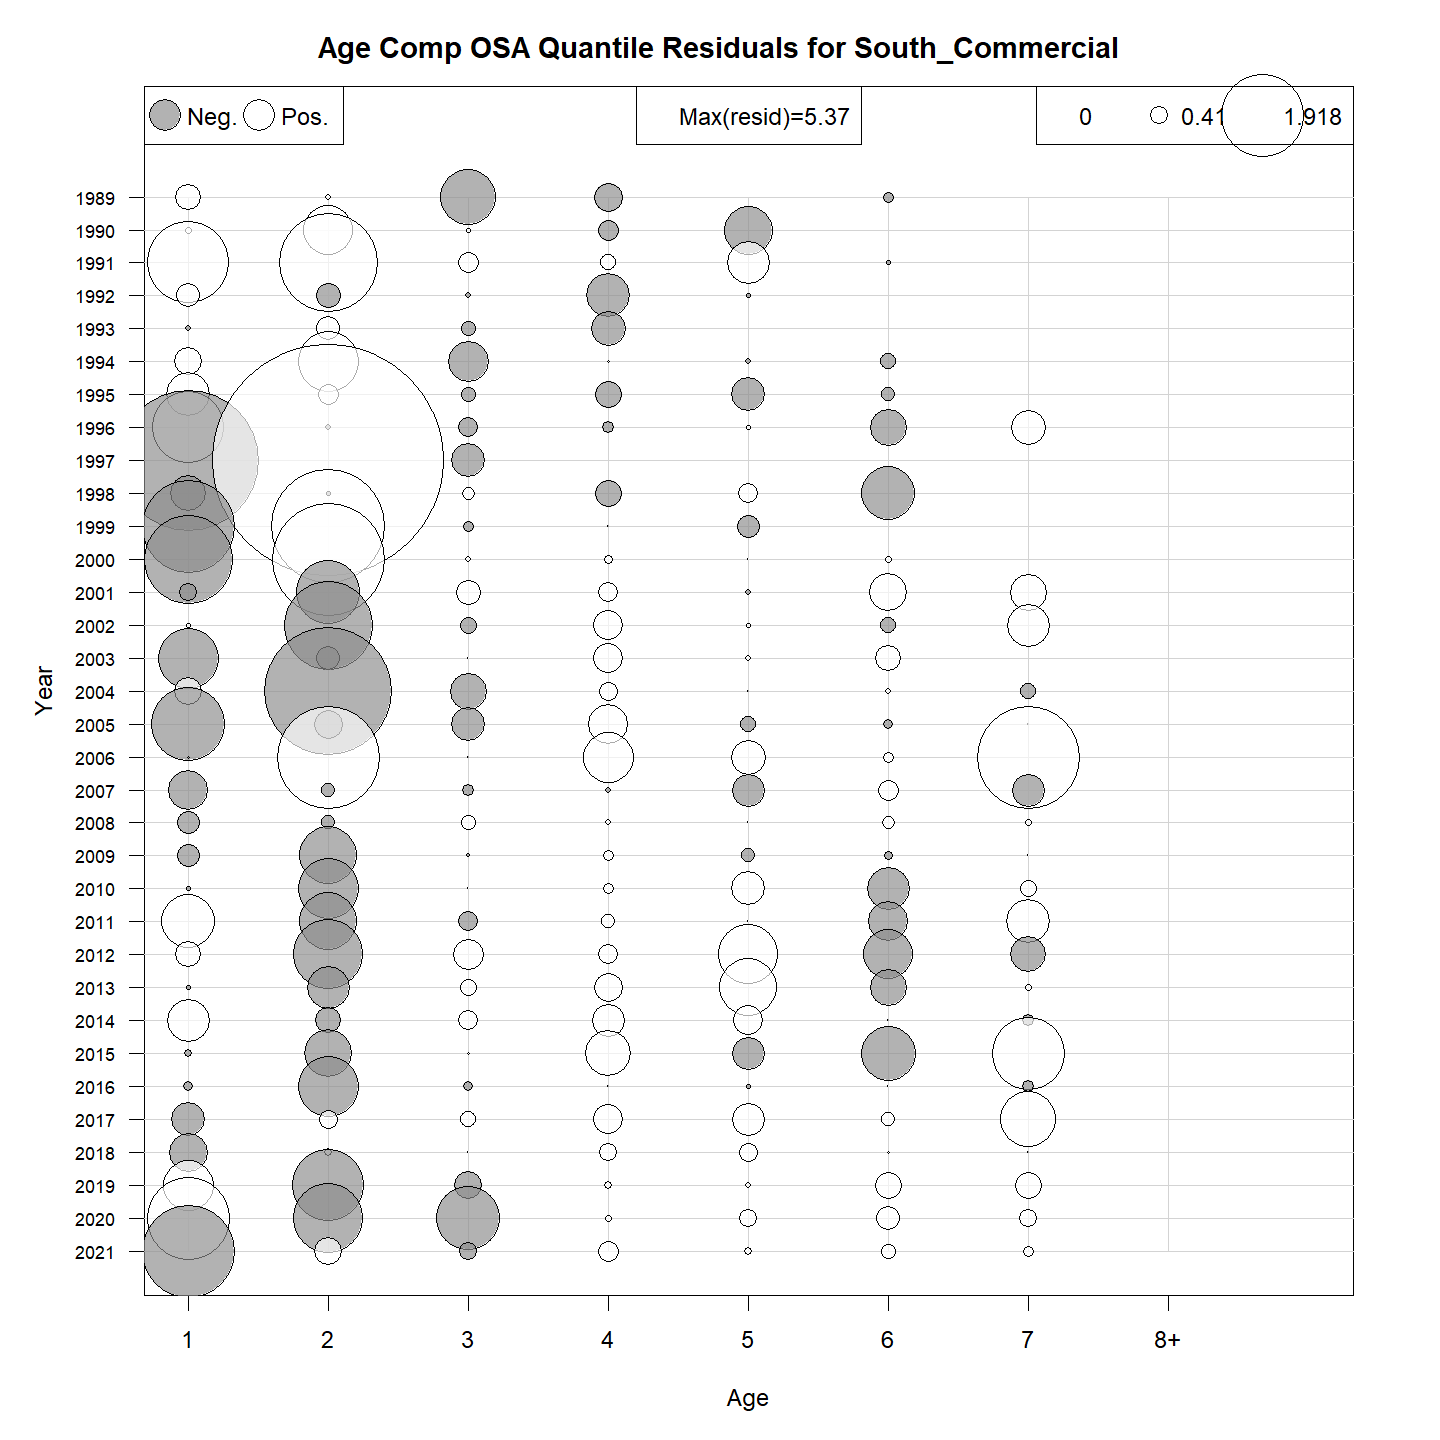
\includegraphics[width=1\linewidth]{../2023.RT.Runs/Run34/plots_png/diagnostics/Catch_age_comp_osa_resids_South_Commercial} 

}

\caption{One-step-ahead residuals for age composition of the Southern commercial fleet.}\label{fig:osa-South-comm-paa}
\end{figure}

\begin{figure}

{\centering 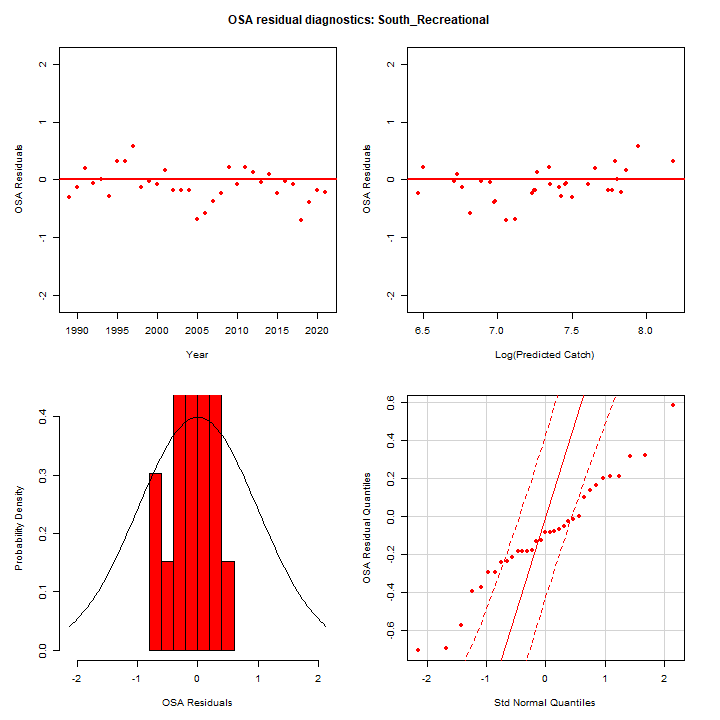
\includegraphics[width=1\linewidth]{../2023.RT.Runs/Run34/plots_png/diagnostics/OSA_resid_catch_4panel_South_Recreational} 

}

\caption{Summary plots for aggregate catch one-step-ahead residuals for the Southern recreational fleet.}\label{fig:osa-South-rec-catch-summ}
\end{figure}
\begin{figure}

{\centering 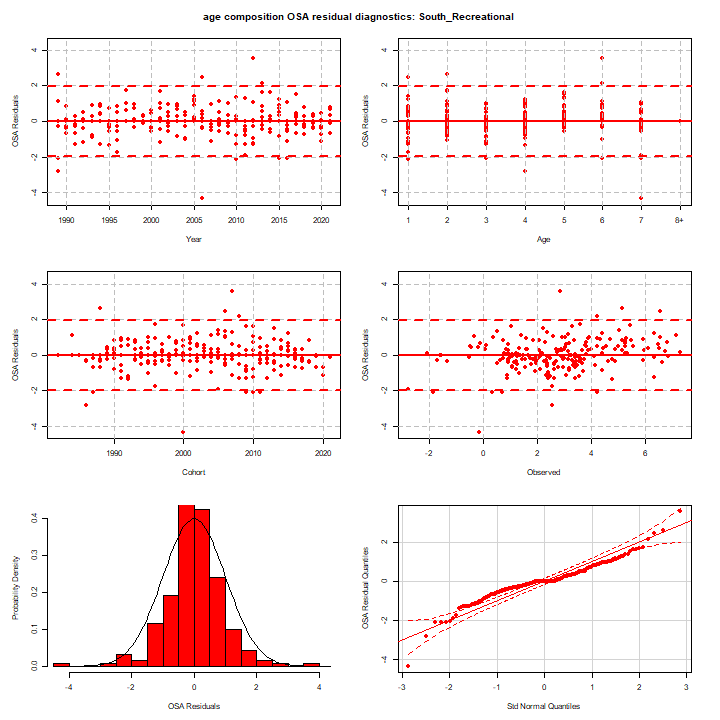
\includegraphics[width=1\linewidth]{../2023.RT.Runs/Run34/plots_png/diagnostics/OSA_resid_paa_6panel_South_Recreational} 

}

\caption{Summary plots for age composition one-step-ahead residuals for the Southern recreational fleet.}\label{fig:osa-South-rec-paa-summ}
\end{figure}
\begin{figure}

{\centering 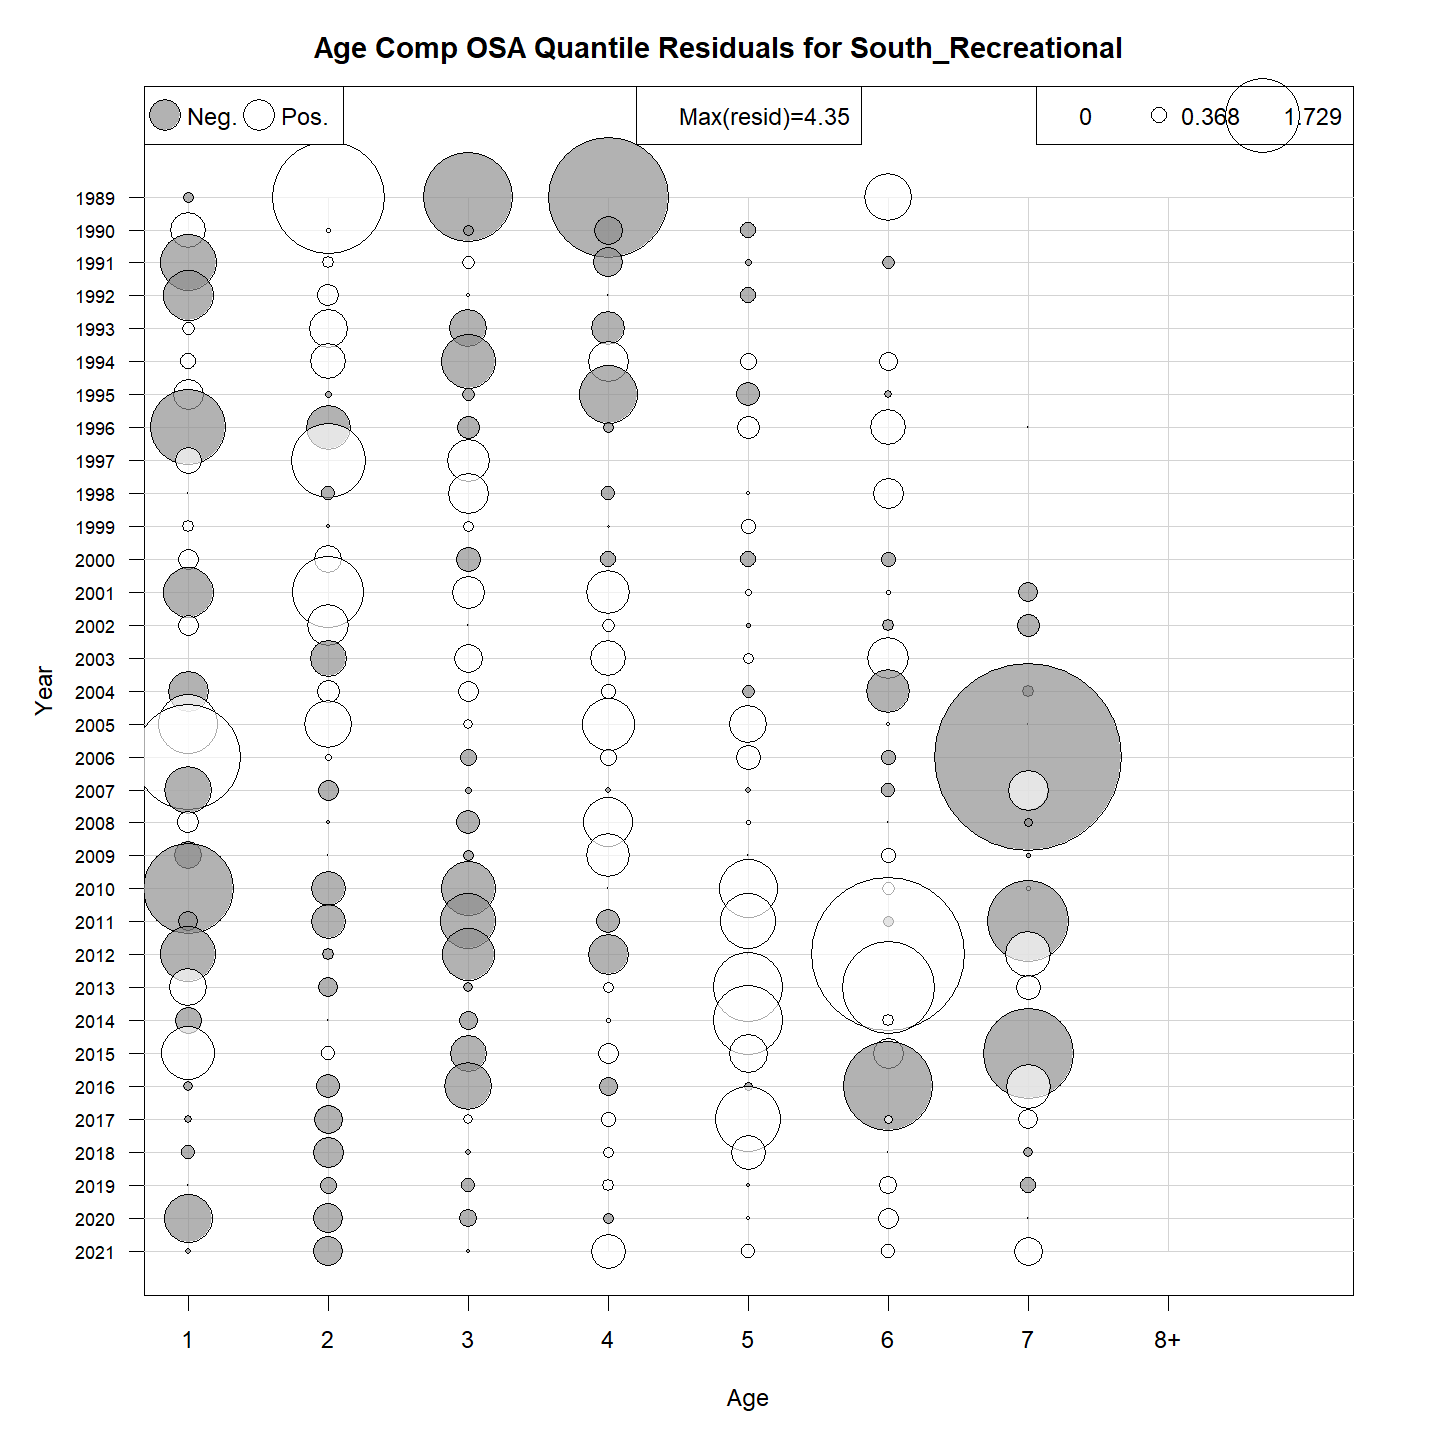
\includegraphics[width=1\linewidth]{../2023.RT.Runs/Run34/plots_png/diagnostics/Catch_age_comp_osa_resids_South_Recreational} 

}

\caption{One-step-ahead residuals for age composition of the Southern recreational fleet.}\label{fig:osa-South-rec-paa}
\end{figure}

\begin{figure}

{\centering 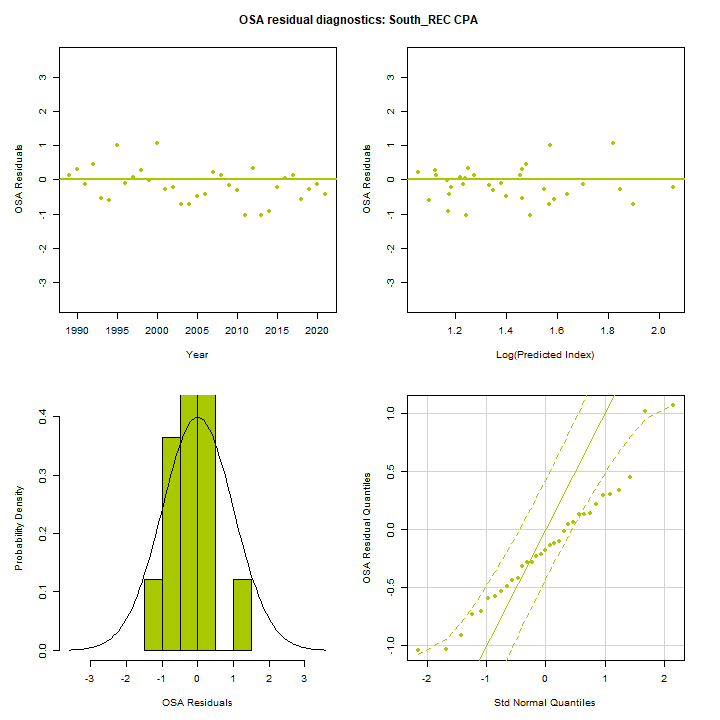
\includegraphics[width=1\linewidth]{../2023.RT.Runs/Run34/plots_png/diagnostics/OSA_resid_catch_4panel_South_REC_CPA} 

}

\caption{Summary plots for aggregate catch one-step-ahead residuals for the Southern Recreational CPA index.}\label{fig:osa-South-reccpa-catch-summ}
\end{figure}
\begin{figure}

{\centering 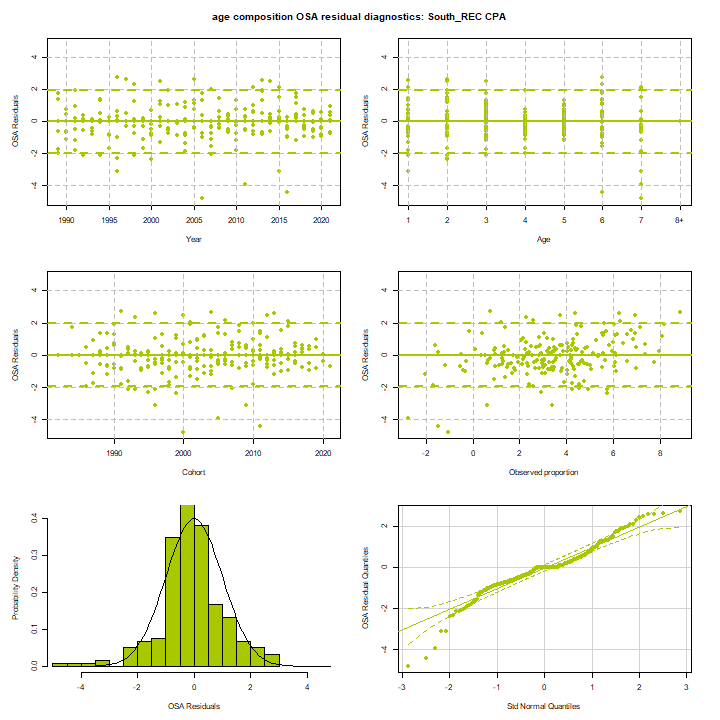
\includegraphics[width=1\linewidth]{../2023.RT.Runs/Run34/plots_png/diagnostics/OSA_resid_paa_6panel_South_REC_CPA} 

}

\caption{Summary plots for age composition one-step-ahead residuals for the Southern Recreational CPA index.}\label{fig:osa-South-reccpa-paa-summ}
\end{figure}
\begin{figure}

{\centering 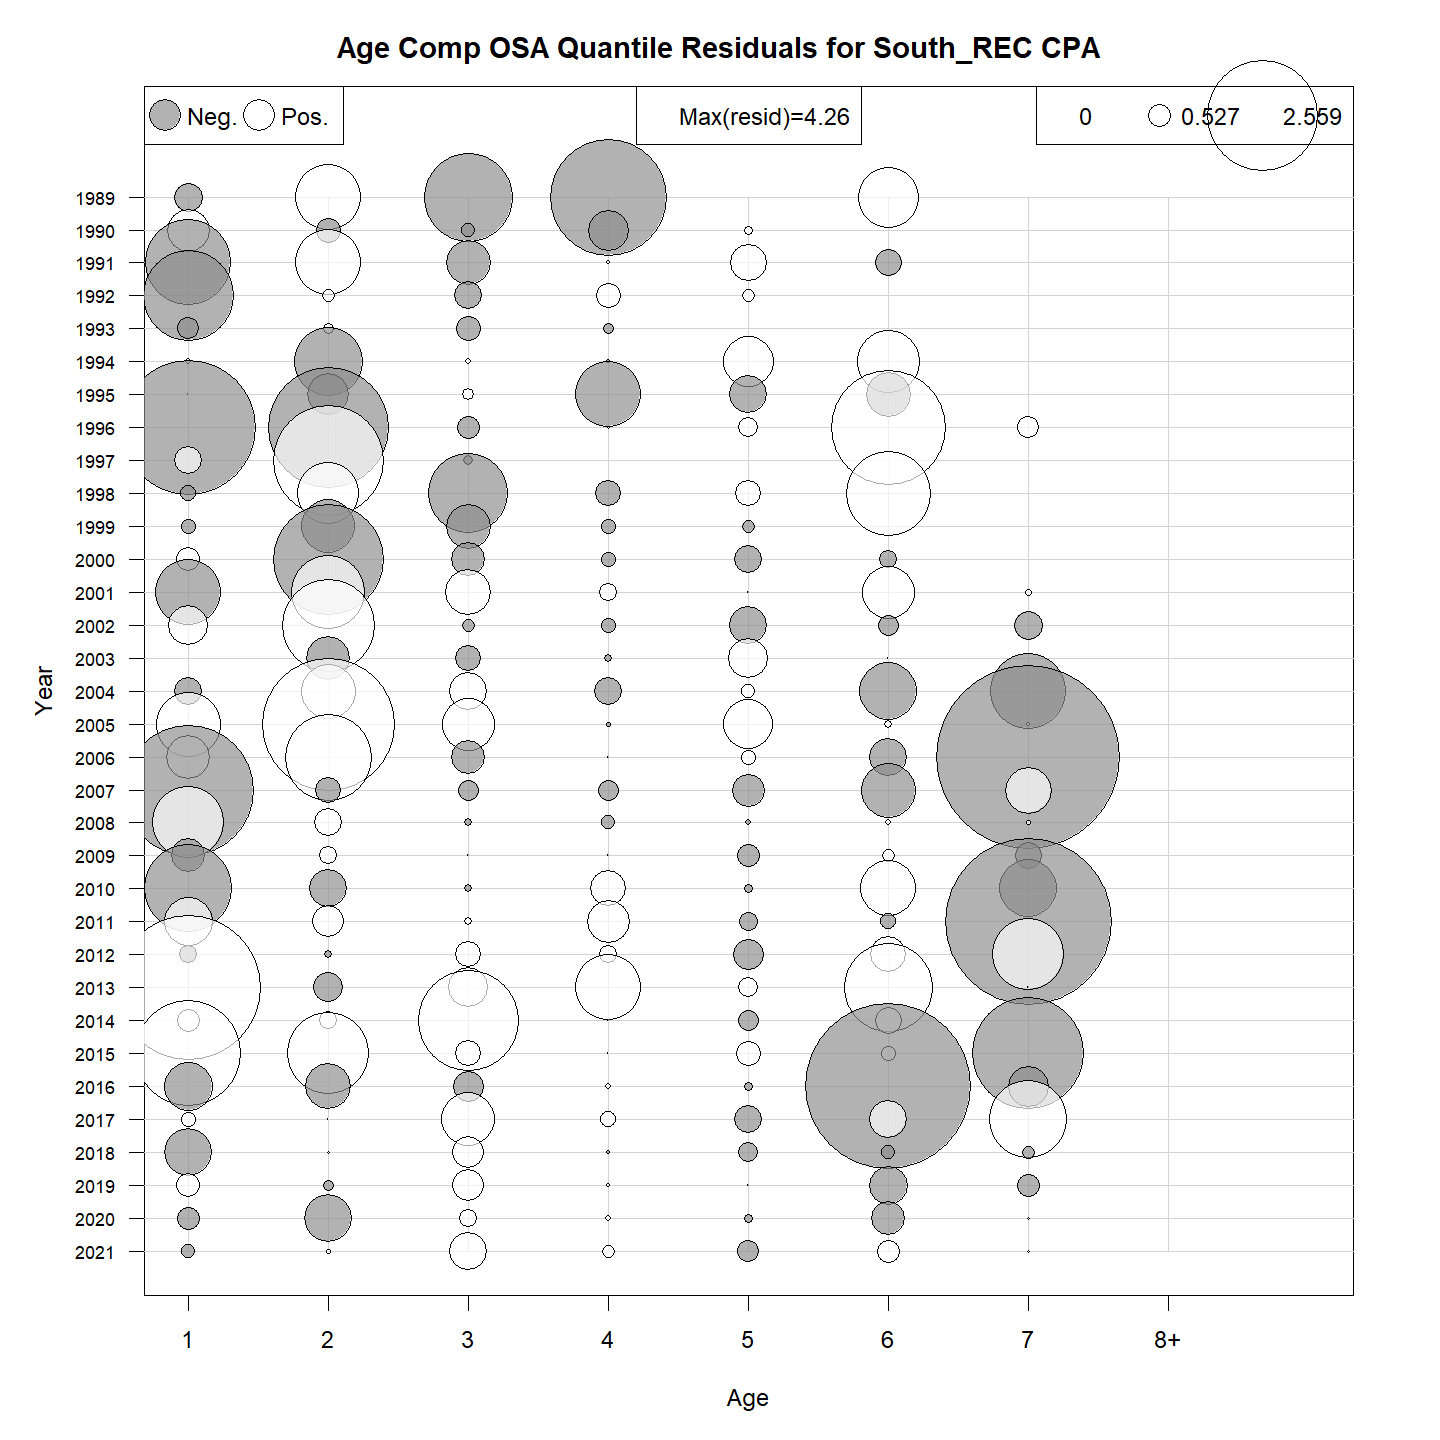
\includegraphics[width=1\linewidth]{../2023.RT.Runs/Run34/plots_png/diagnostics/Catch_age_comp_osa_resids_South_REC_CPA} 

}

\caption{One-step-ahead residuals for age composition of the Southern Recreational CPA index.}\label{fig:osa-South-reccpa-paa}
\end{figure}

\begin{figure}

{\centering 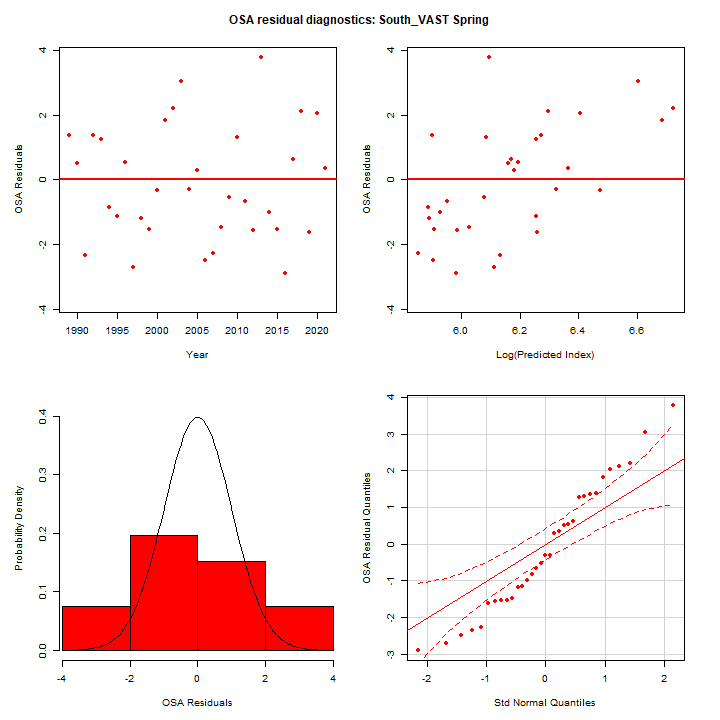
\includegraphics[width=1\linewidth]{../2023.RT.Runs/Run34/plots_png/diagnostics/OSA_resid_catch_4panel_South_VAST_Spring} 

}

\caption{Summary plots for aggregate catch one-step-ahead residuals for the Southern VAST index.}\label{fig:osa-South-vast-catch-summ}
\end{figure}
\begin{figure}

{\centering 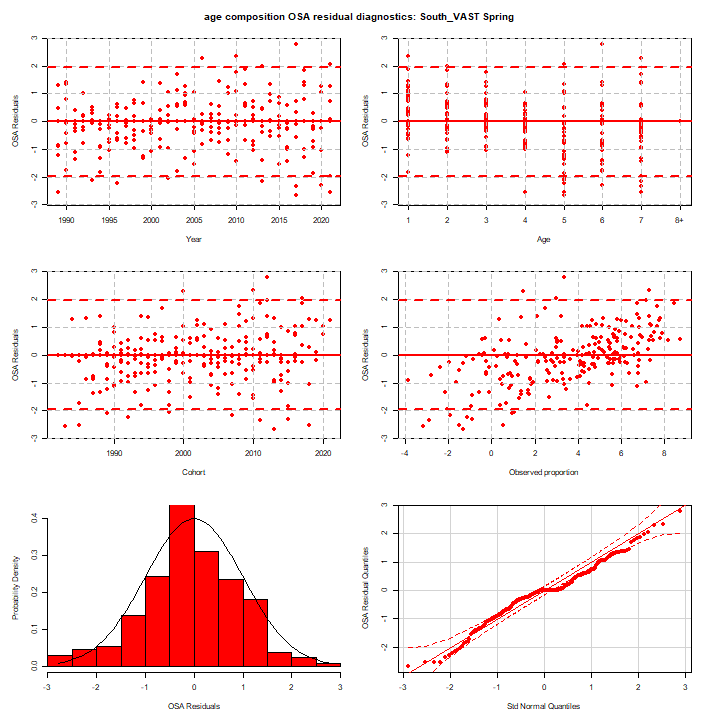
\includegraphics[width=1\linewidth]{../2023.RT.Runs/Run34/plots_png/diagnostics/OSA_resid_paa_6panel_South_VAST_Spring} 

}

\caption{Summary plots for age composition one-step-ahead residuals for the Southern VAST index.}\label{fig:osa-South-vast-paa-summ}
\end{figure}
\begin{figure}

{\centering 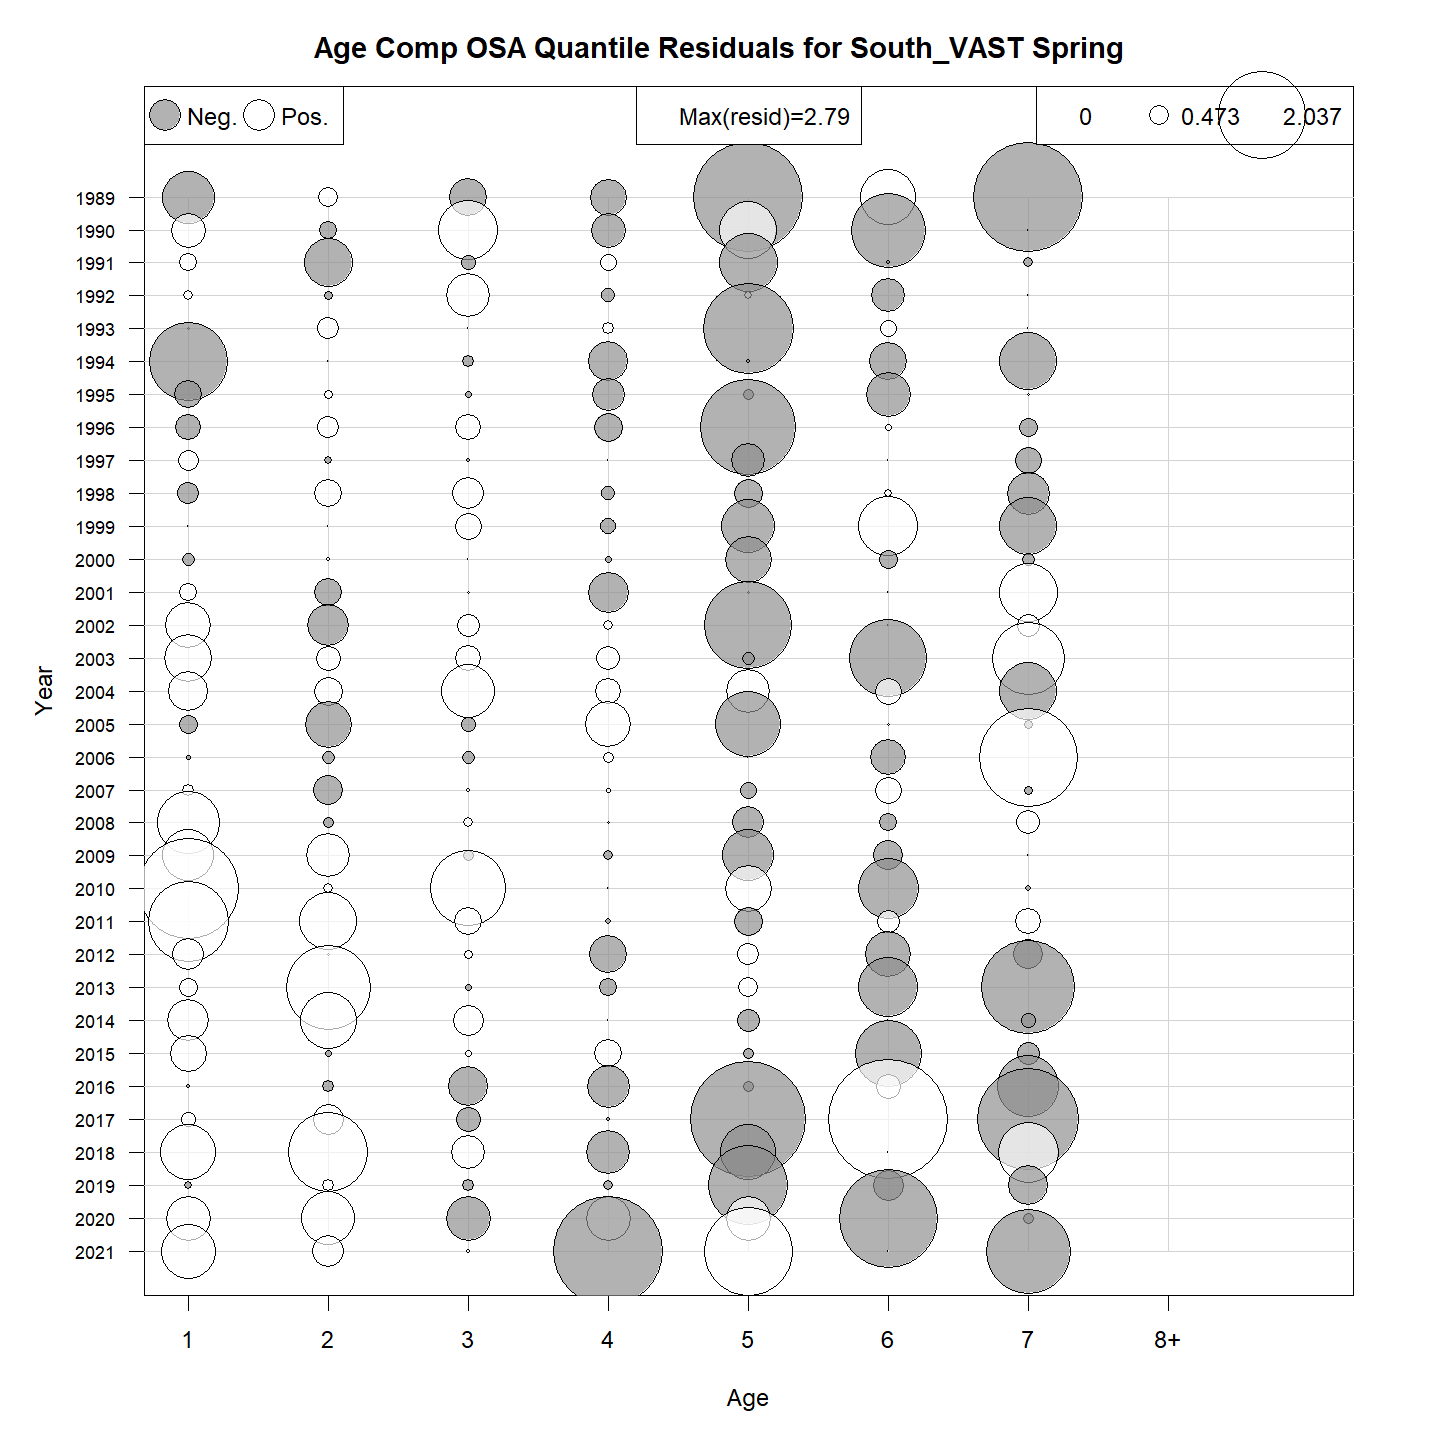
\includegraphics[width=1\linewidth]{../2023.RT.Runs/Run34/plots_png/diagnostics/Catch_age_comp_osa_resids_South_VAST_Spring} 

}

\caption{One-step-ahead residuals for age composition of the Southern VAST index.}\label{fig:osa-South-vast-paa}
\end{figure}

\begin{figure}

{\centering 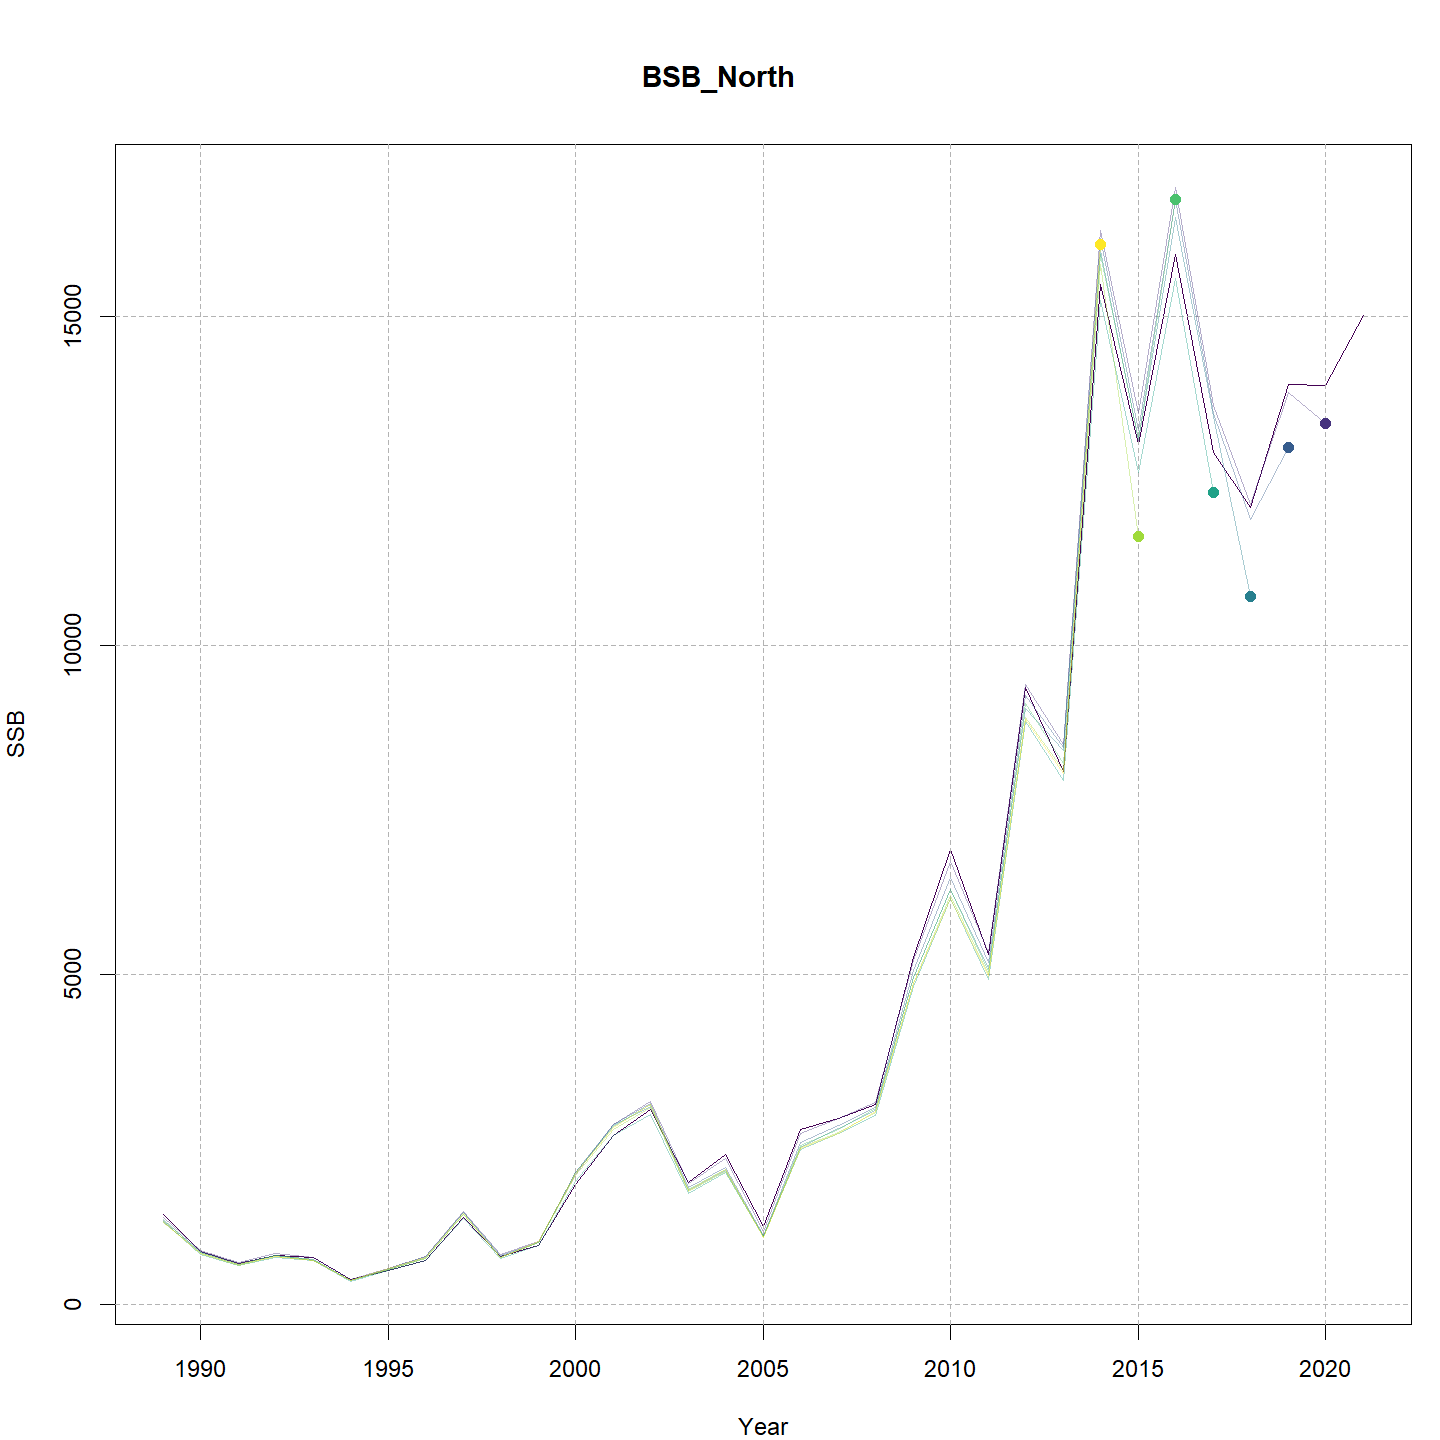
\includegraphics[width=0.65\linewidth]{../2023.RT.Runs/Run34/plots_png/retro/BSB_North_SSB_retro} 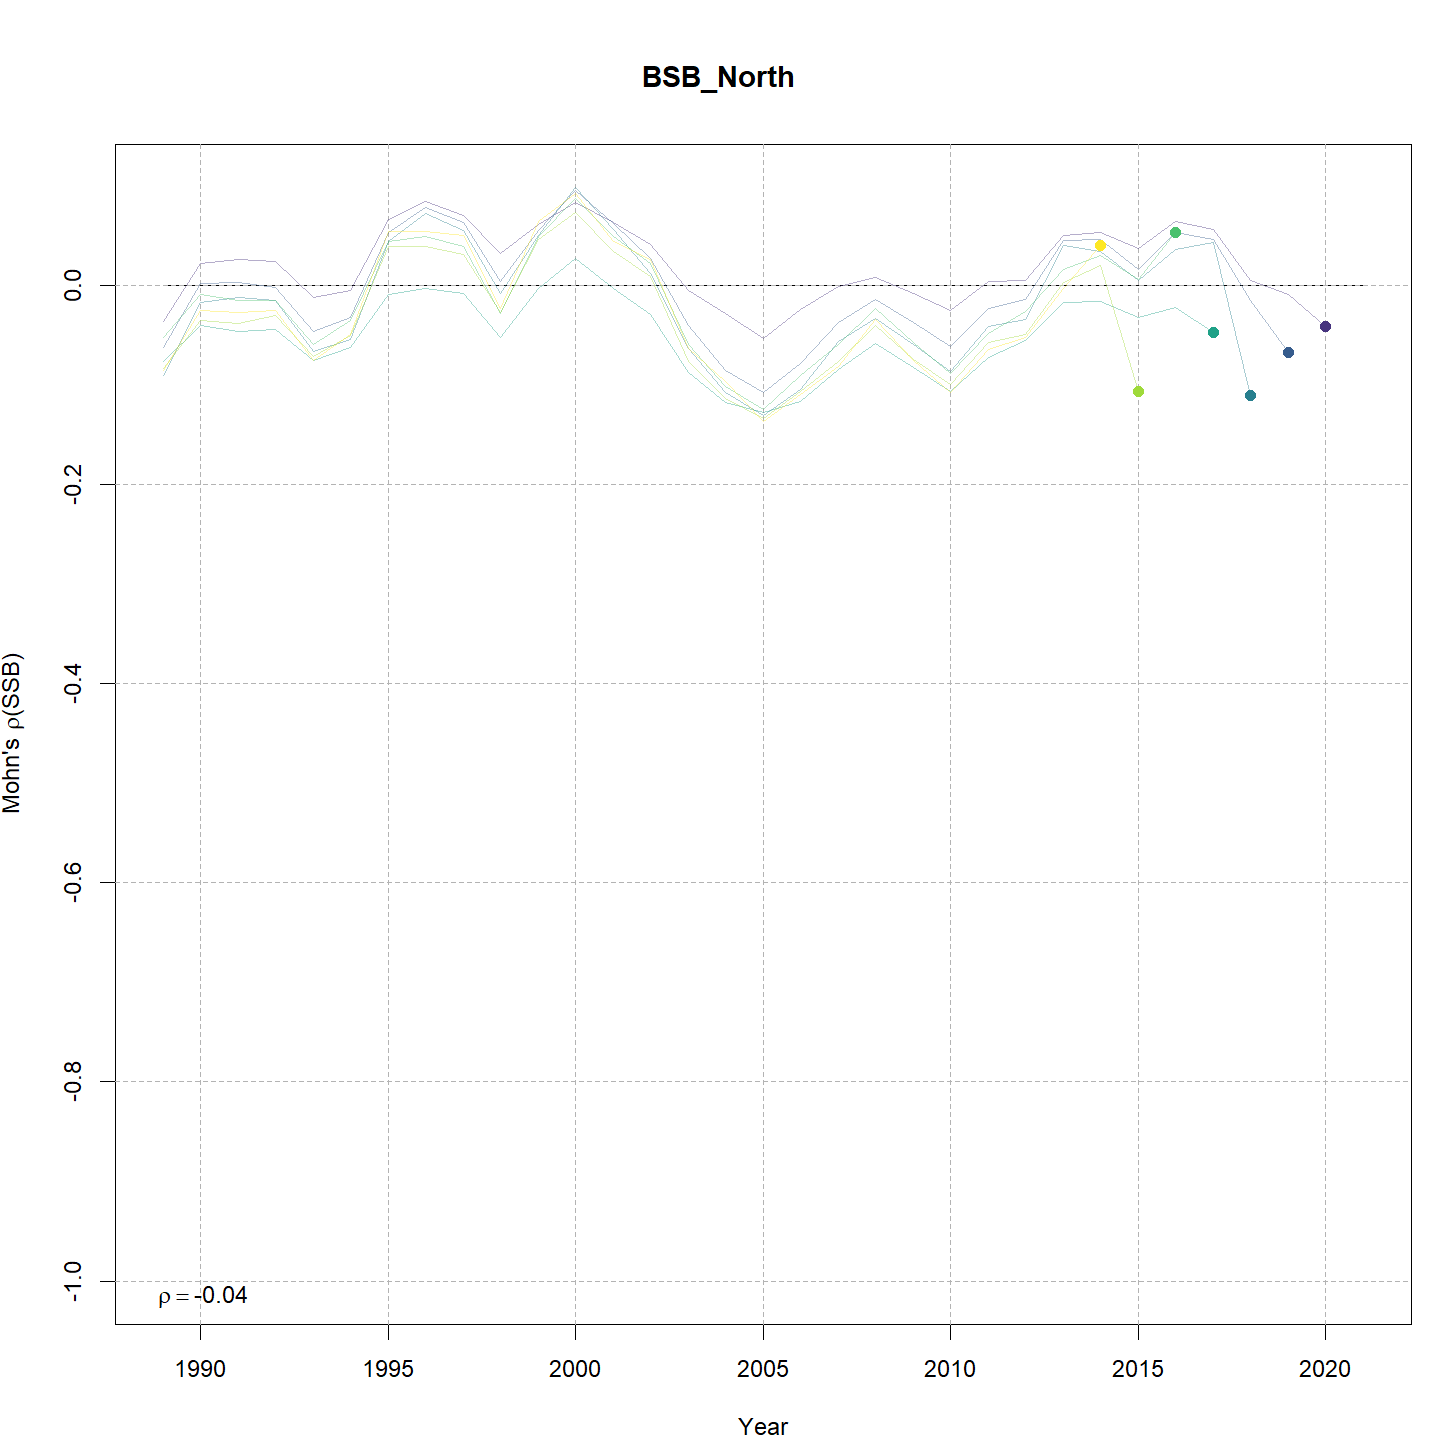
\includegraphics[width=0.65\linewidth]{../2023.RT.Runs/Run34/plots_png/retro/BSB_North_SSB_retro_relative} 

}

\caption{Retrospective patterns for SSB of the northern component.}\label{fig:North-retro-ssb}
\end{figure}
\begin{figure}

{\centering 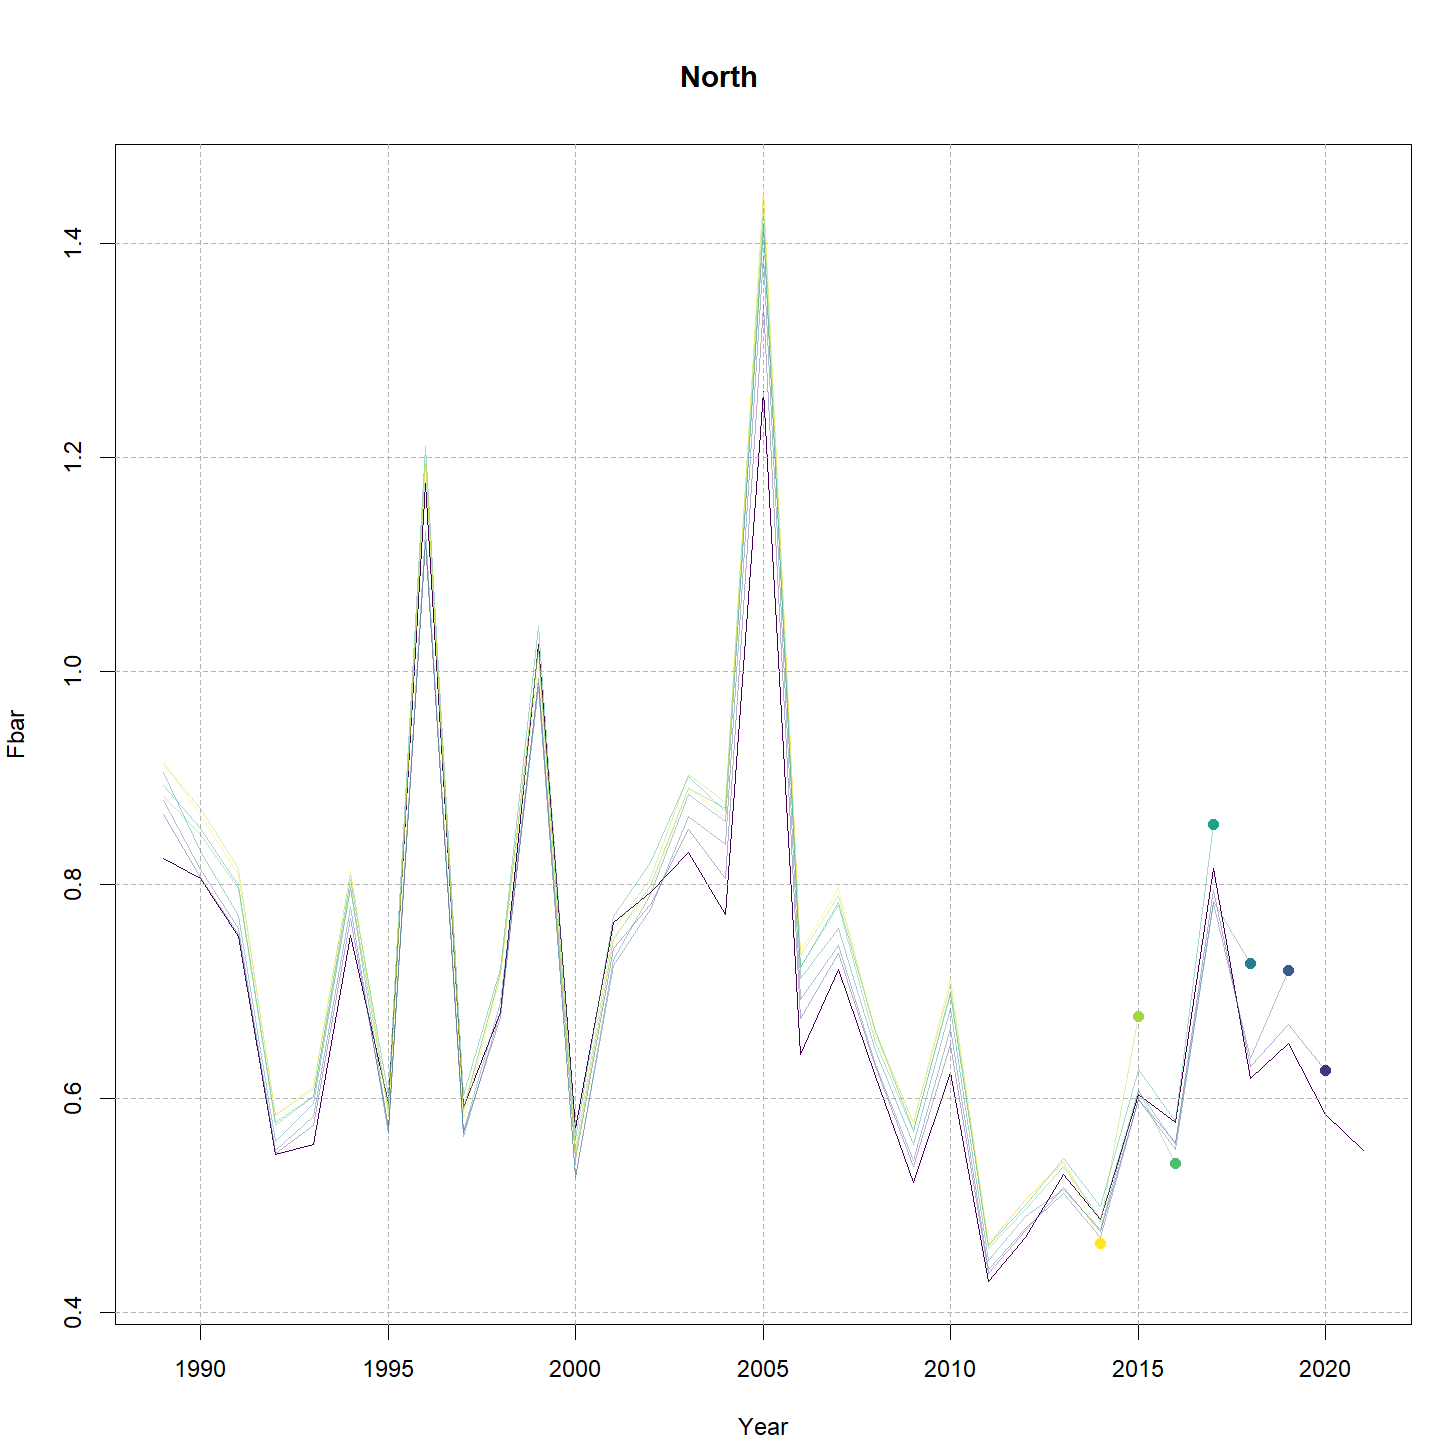
\includegraphics[width=0.65\linewidth]{../2023.RT.Runs/Run34/plots_png/retro/North_Fbar_retro} 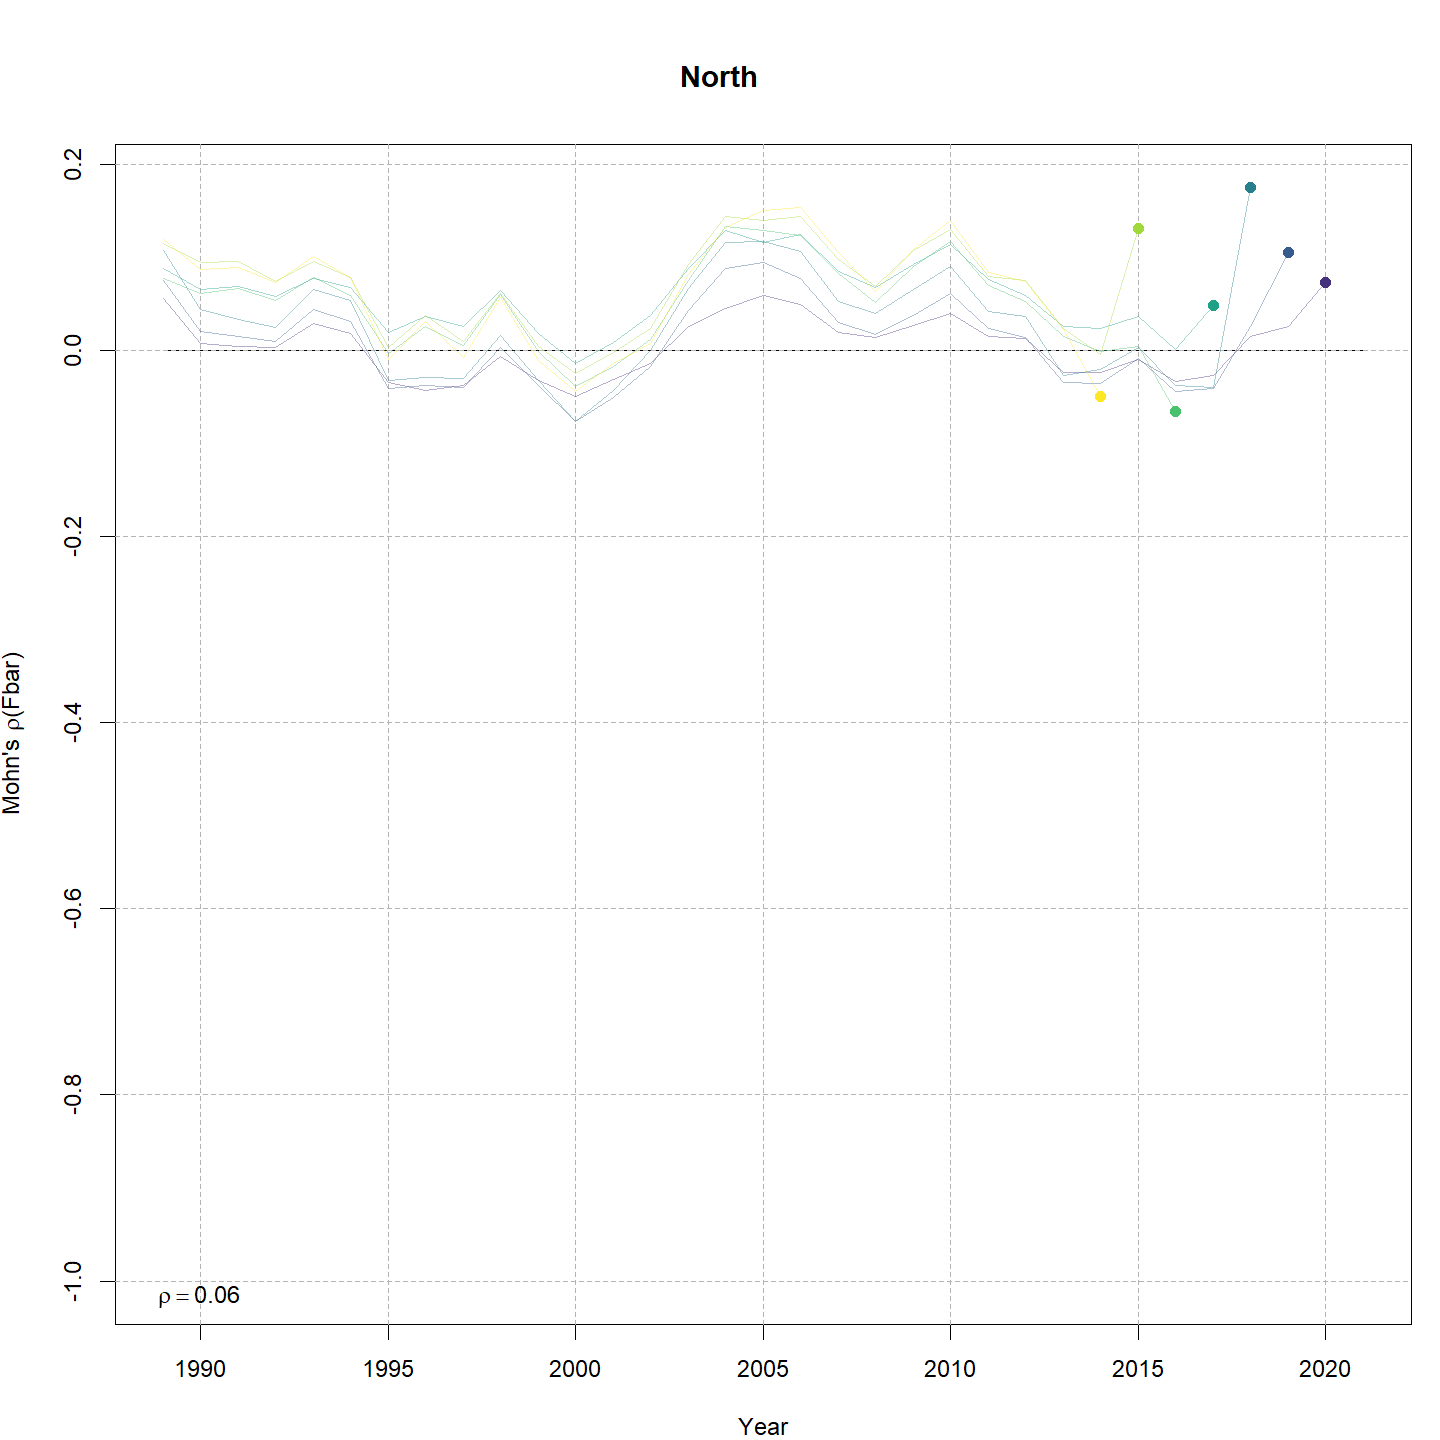
\includegraphics[width=0.65\linewidth]{../2023.RT.Runs/Run34/plots_png/retro/North_Fbar_retro_relative} 

}

\caption{Retrospective patterns for average fishing mortality for ages 6 and 7 in the northern region.}\label{fig:North-retro-F}
\end{figure}

\begin{figure}

{\centering 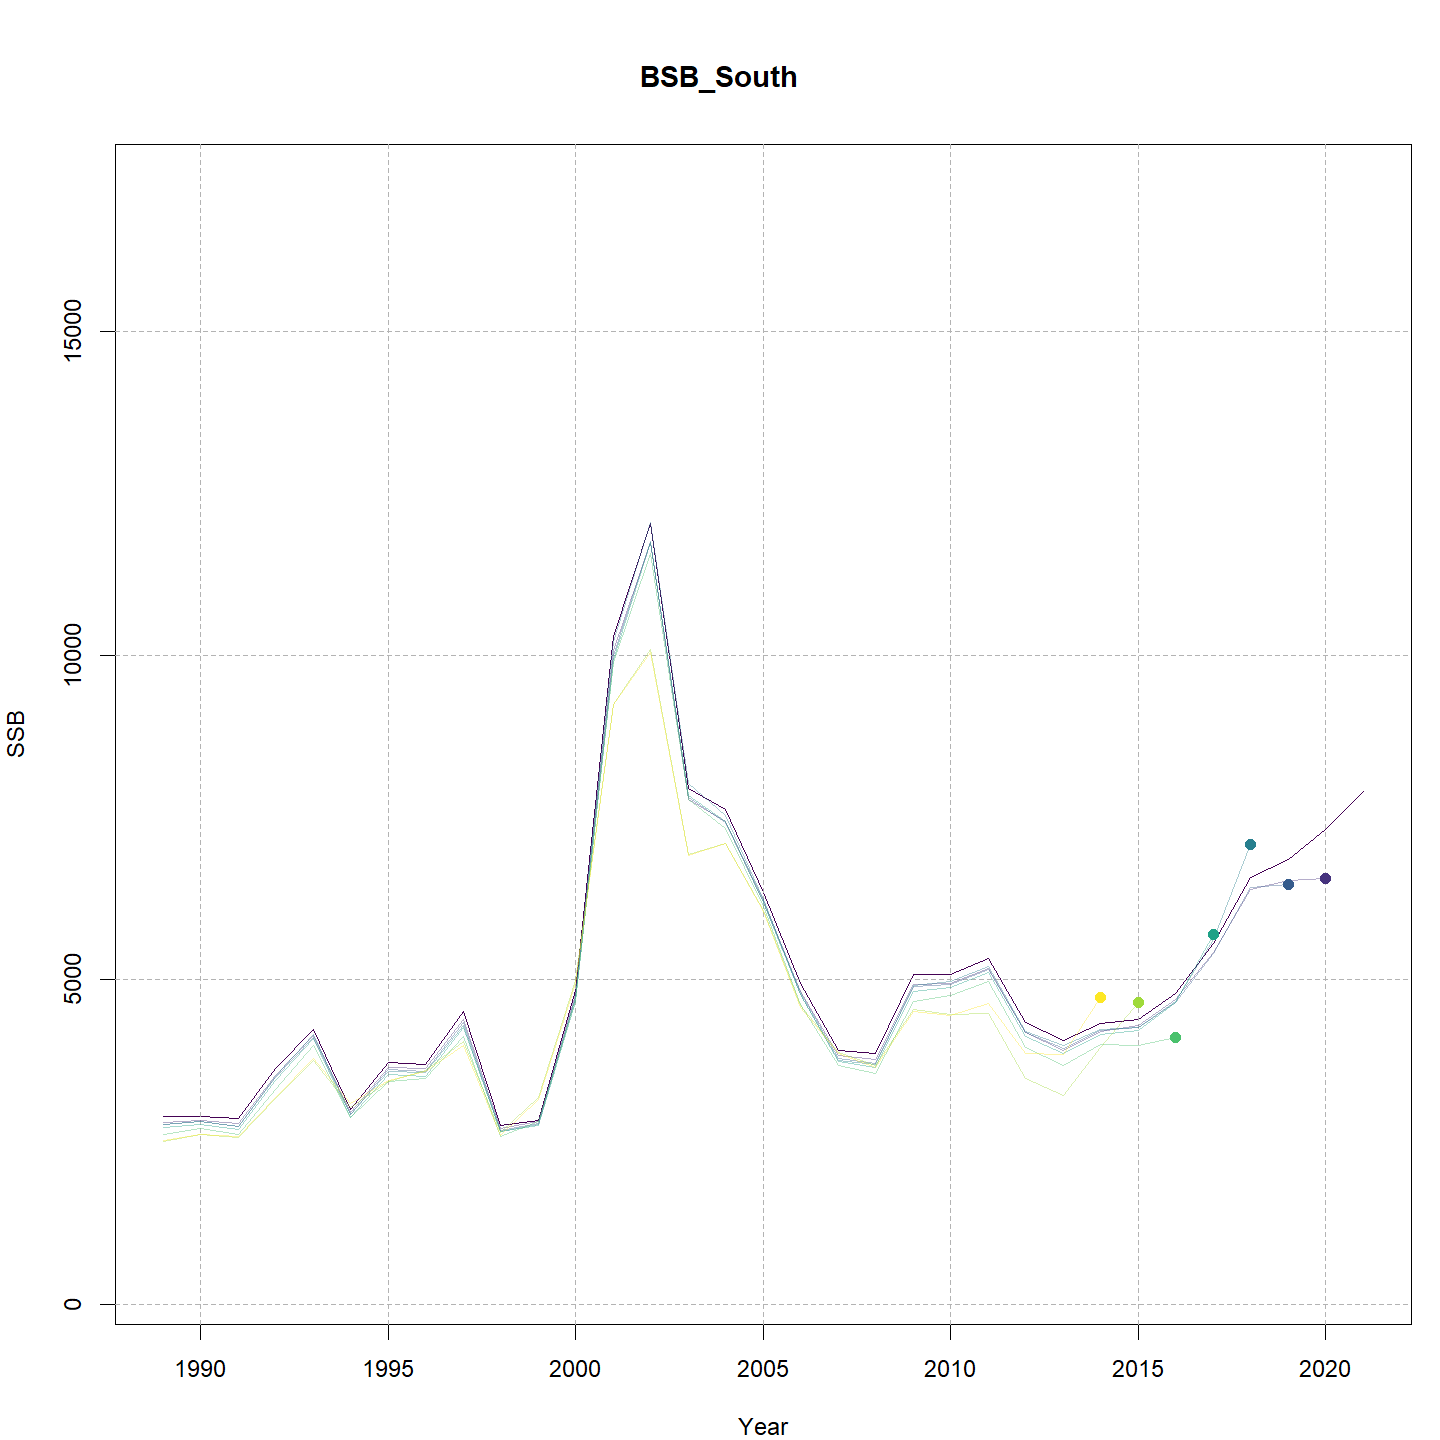
\includegraphics[width=0.65\linewidth]{../2023.RT.Runs/Run34/plots_png/retro/BSB_South_SSB_retro} 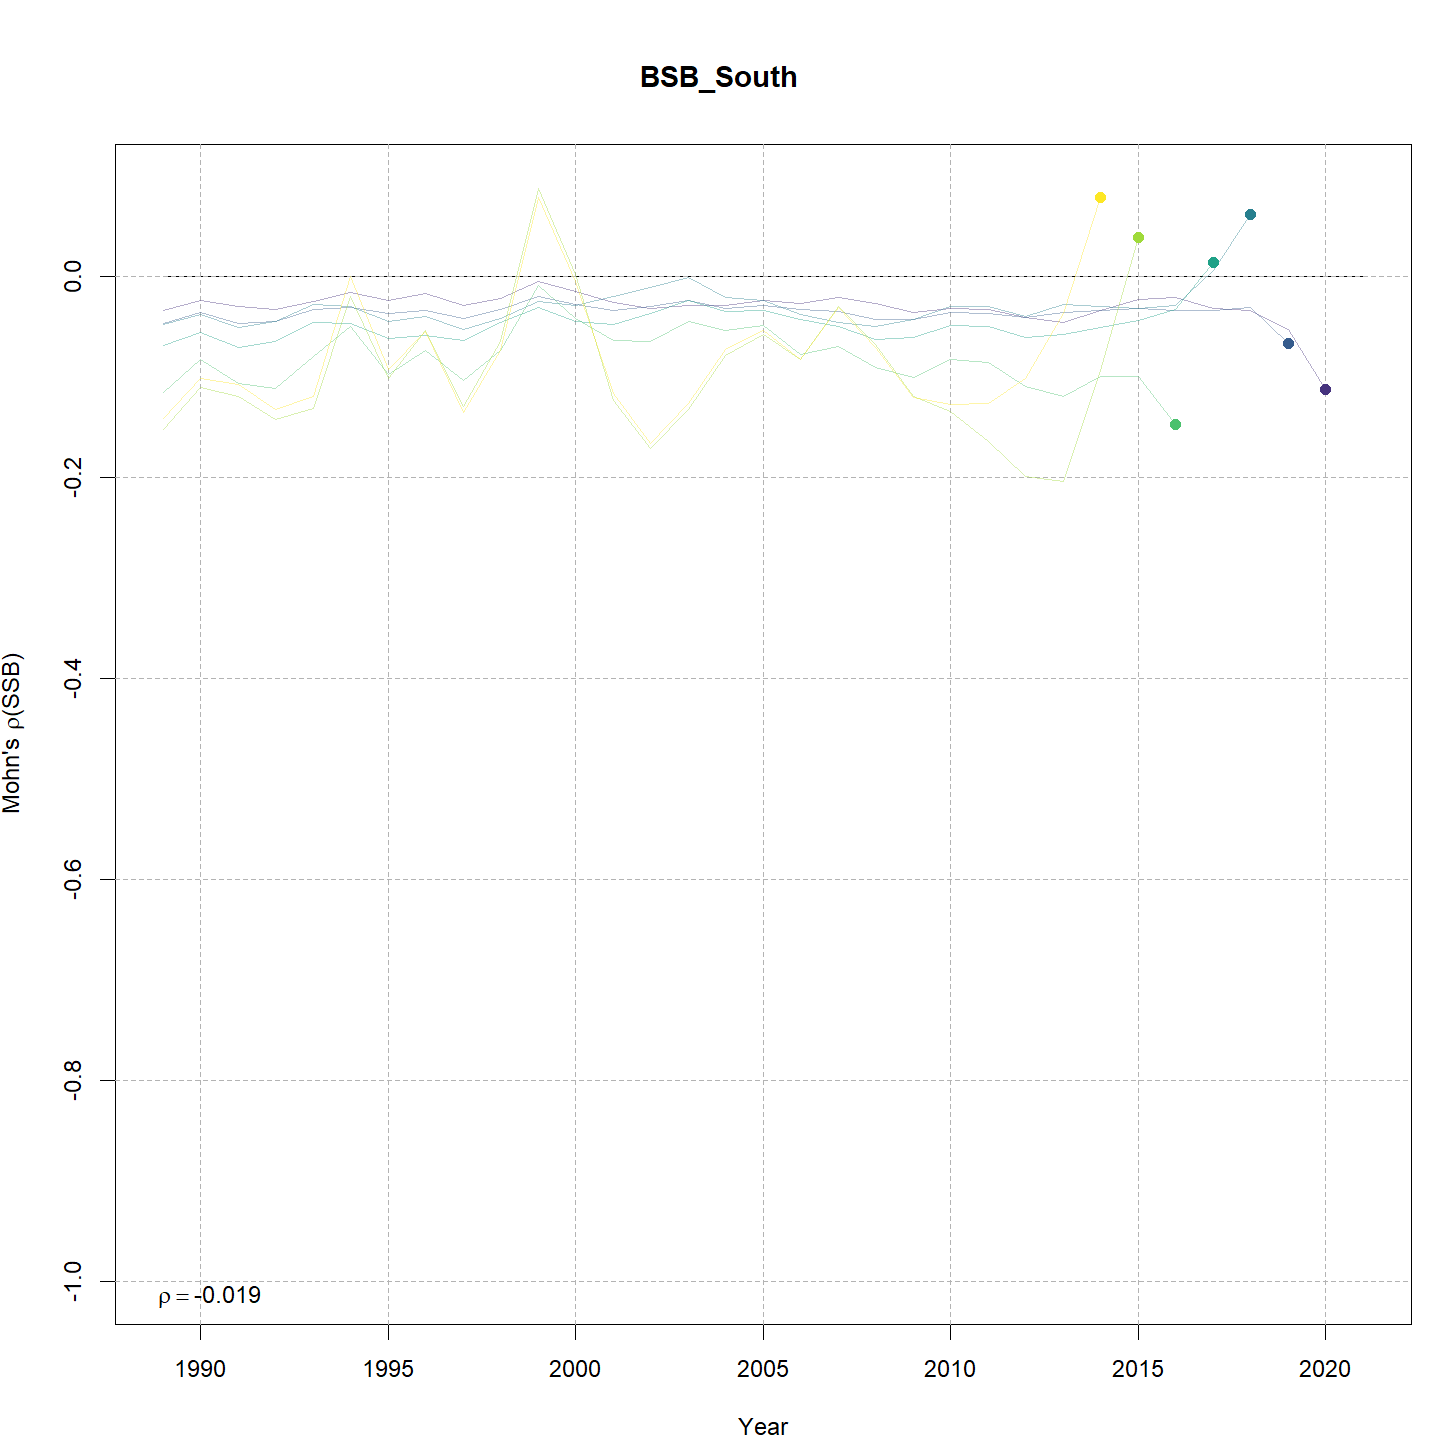
\includegraphics[width=0.65\linewidth]{../2023.RT.Runs/Run34/plots_png/retro/BSB_South_SSB_retro_relative} 

}

\caption{Retrospective patterns for SSB of the southern component.}\label{fig:South-retro-ssb}
\end{figure}
\begin{figure}

{\centering 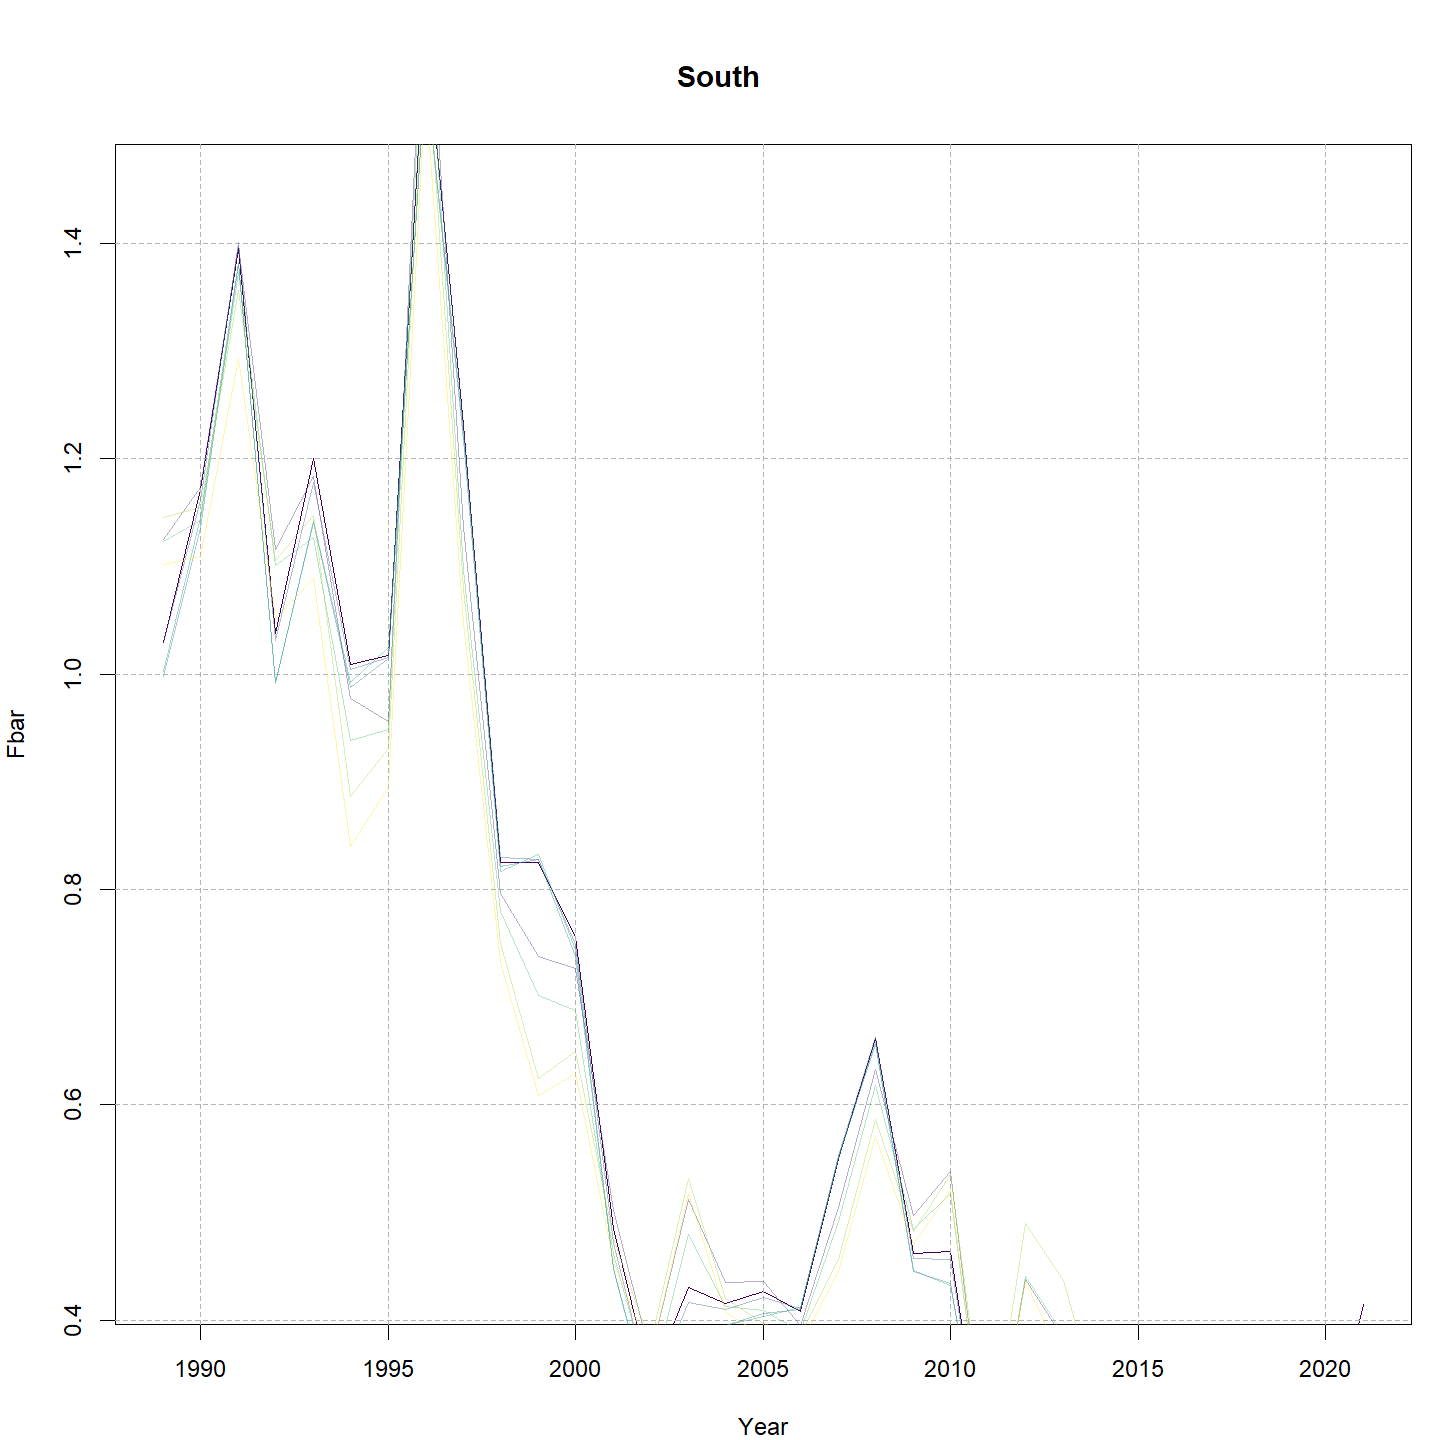
\includegraphics[width=0.65\linewidth]{../2023.RT.Runs/Run34/plots_png/retro/South_Fbar_retro} 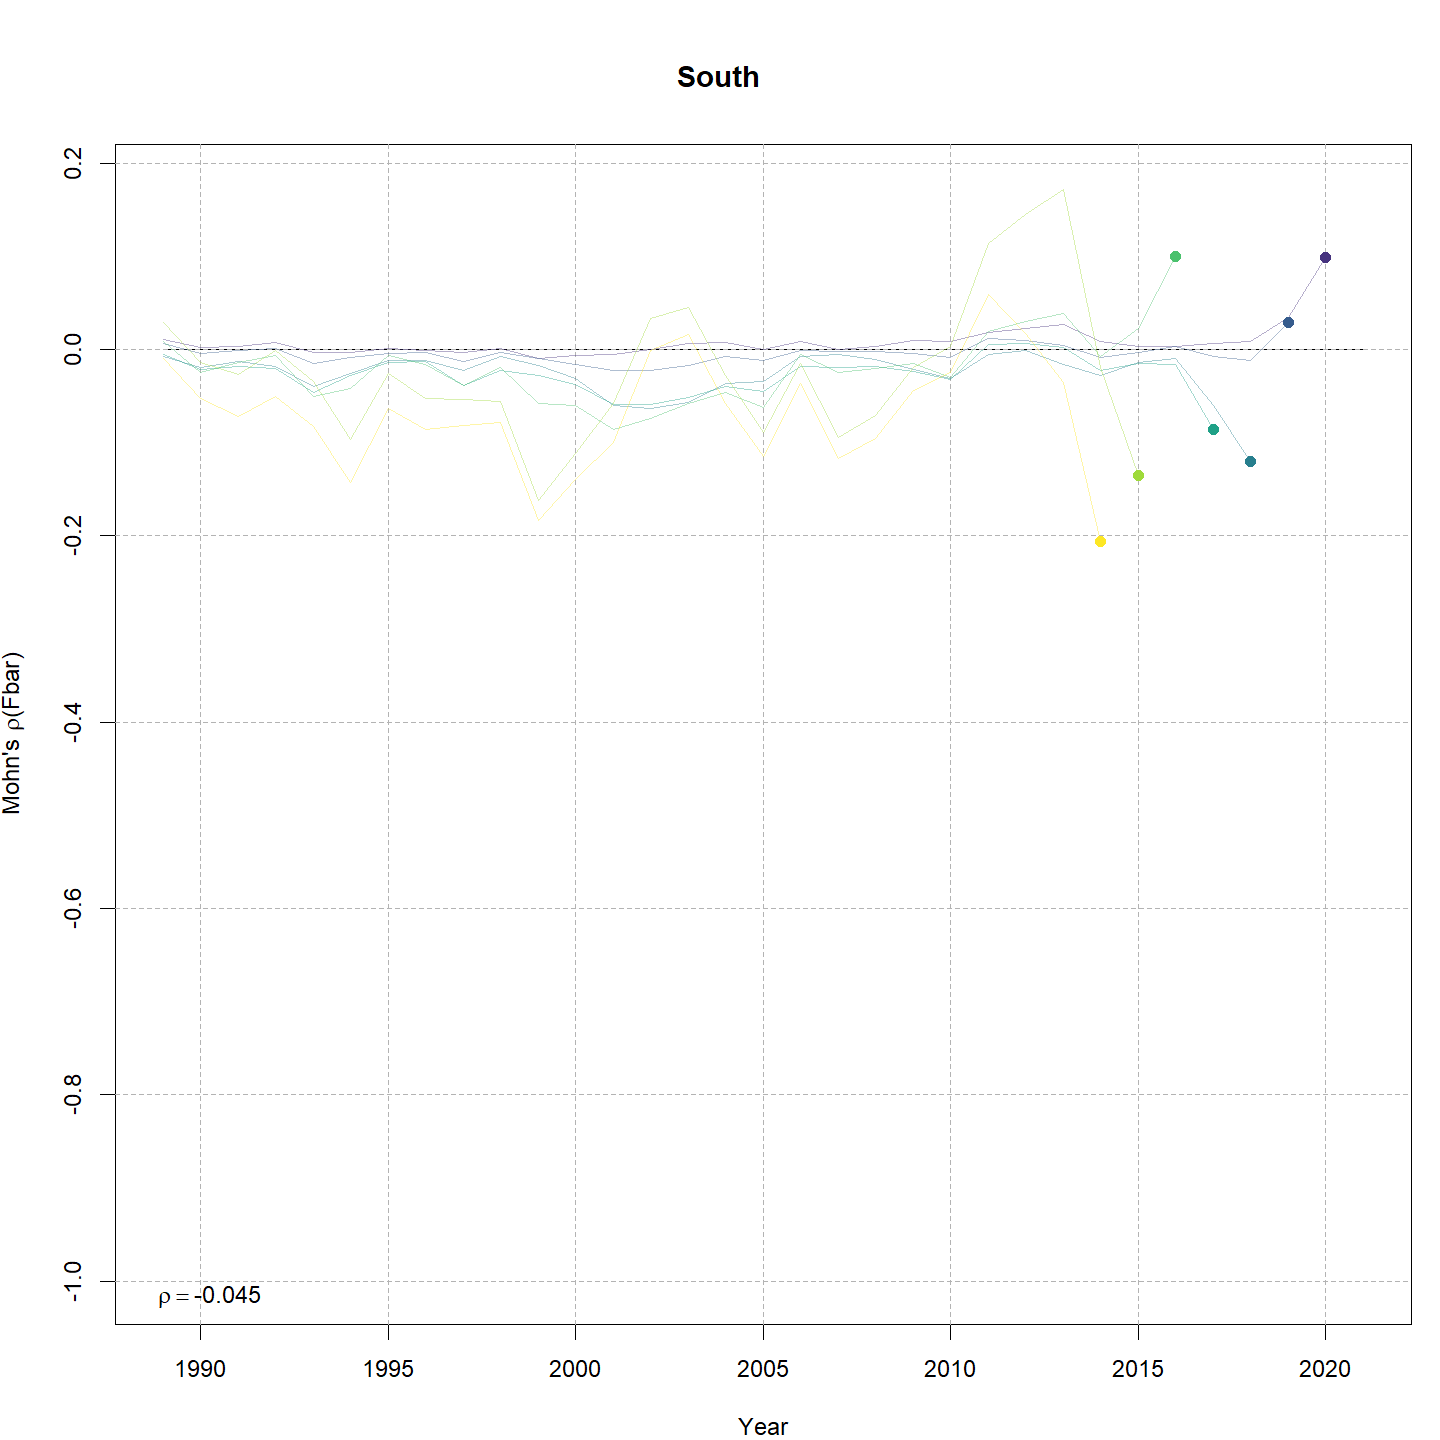
\includegraphics[width=0.65\linewidth]{../2023.RT.Runs/Run34/plots_png/retro/South_Fbar_retro_relative} 

}

\caption{Retrospective patterns for average fishing mortality for ages 6 and 7 in the southern region.}\label{fig:South-retro-F}
\end{figure}

\begin{figure}

{\centering 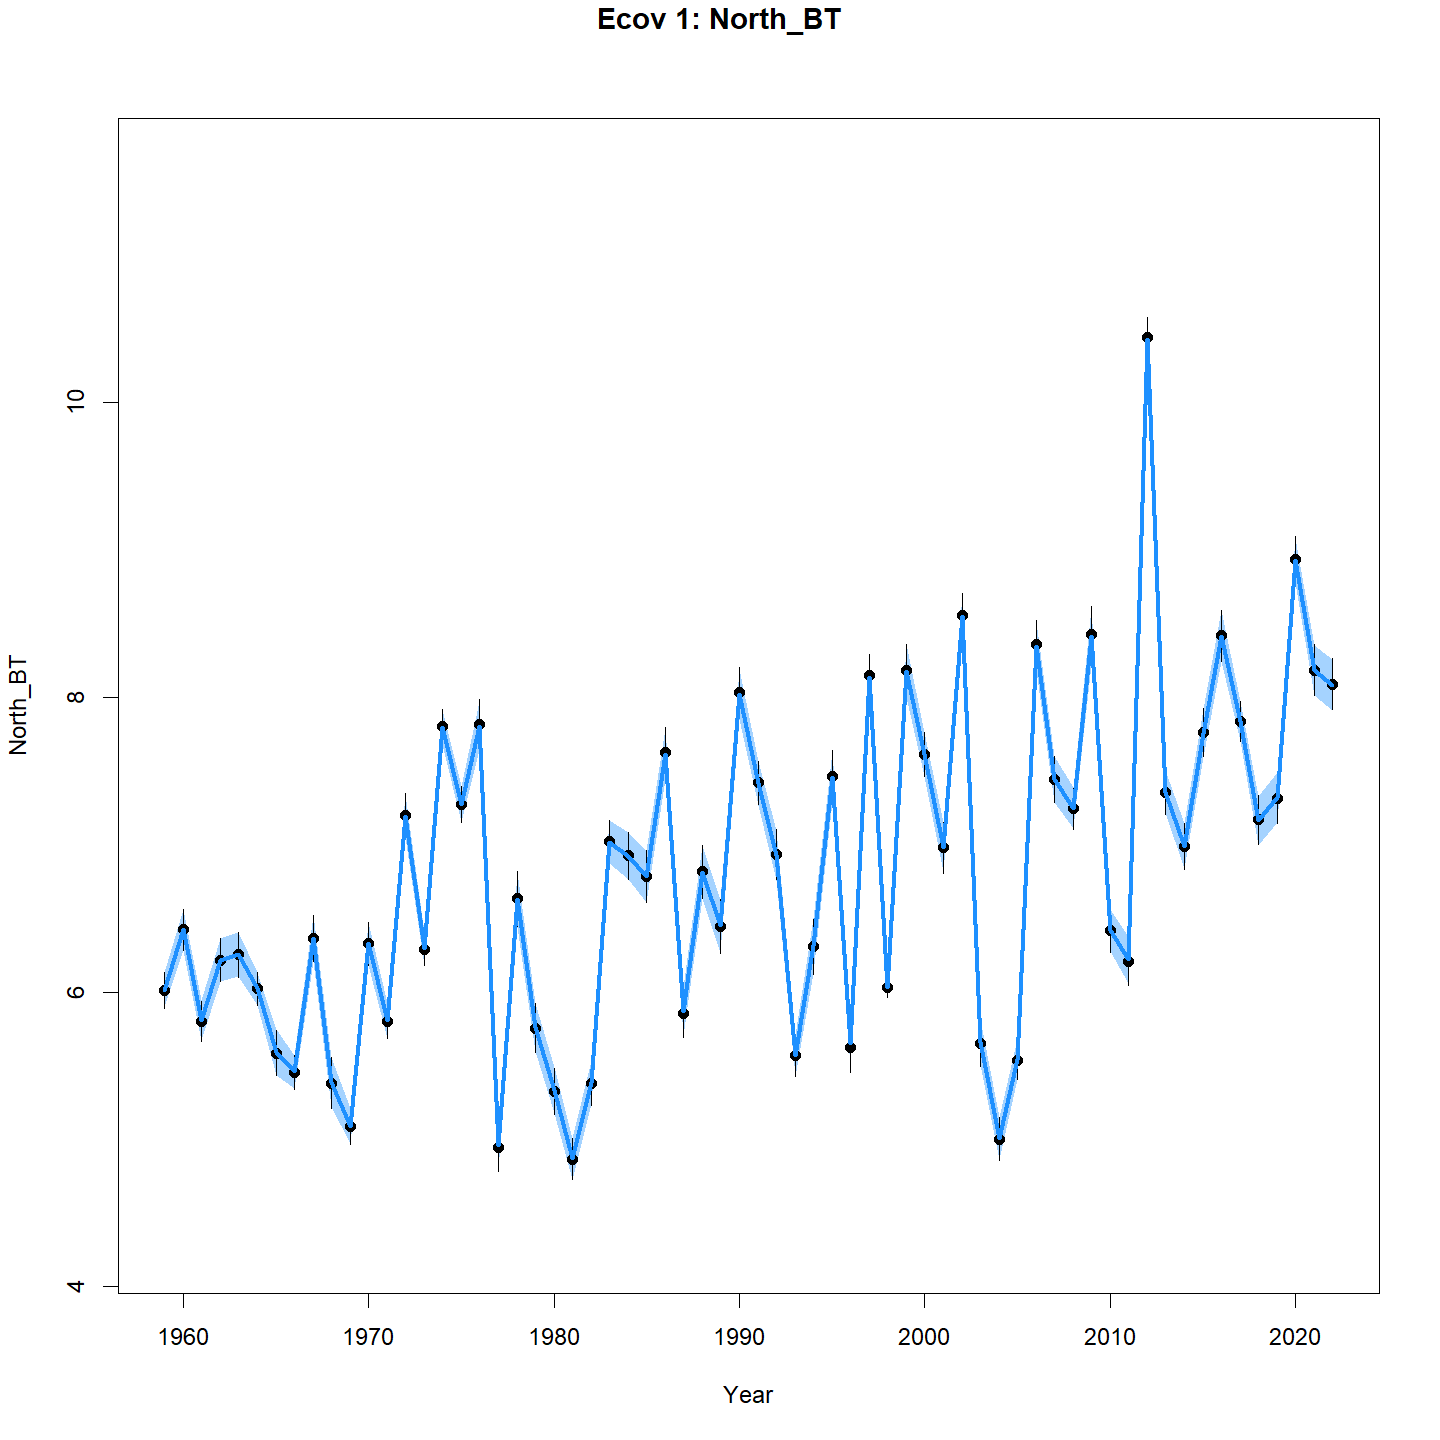
\includegraphics[width=0.65\linewidth]{../2023.RT.Runs/Run34/plots_png/results/Ecov_1_North_BT} 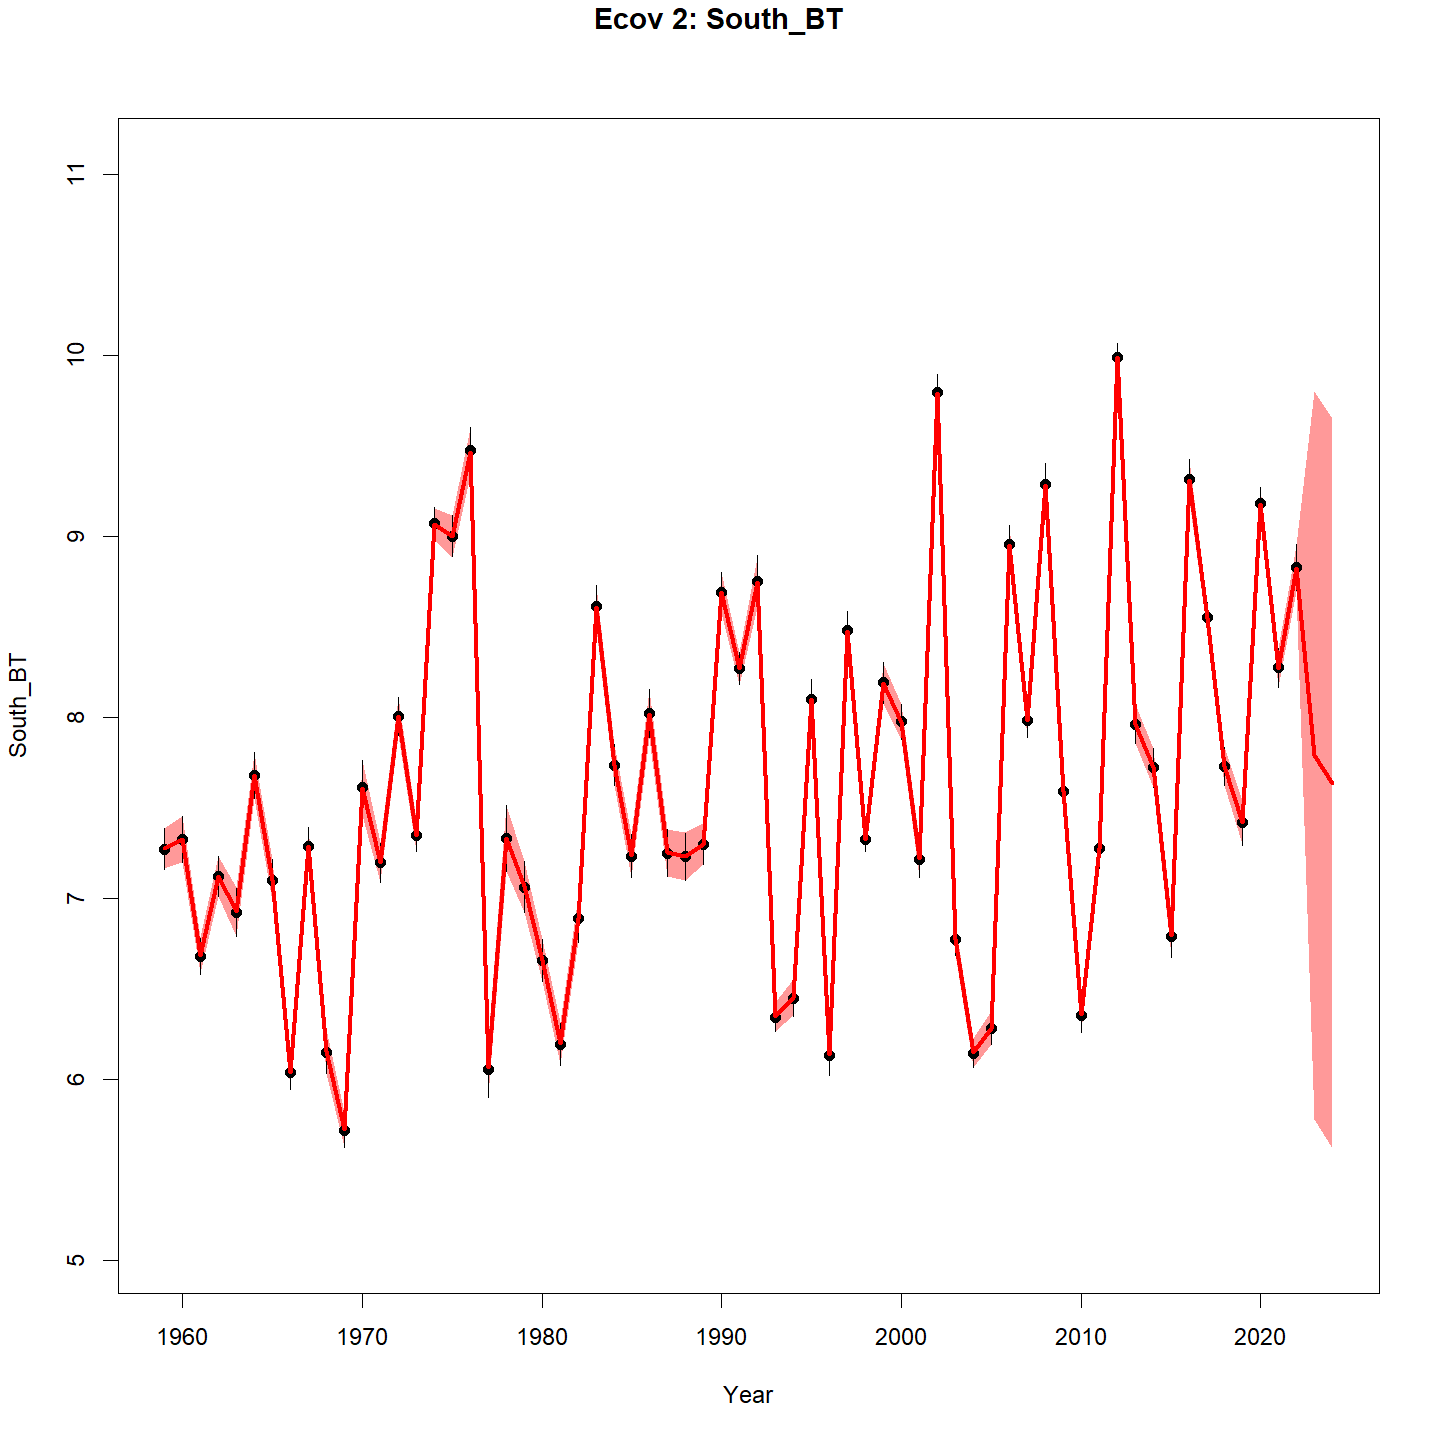
\includegraphics[width=0.65\linewidth]{../2023.RT.Runs/Run34/plots_png/results/Ecov_2_South_BT} 

}

\caption{Observations and estimates of the bottom temperature covariates in the northern and southern regions from the proposed base model.}\label{fig:bottom-temp}
\end{figure}

\begin{figure}

{\centering 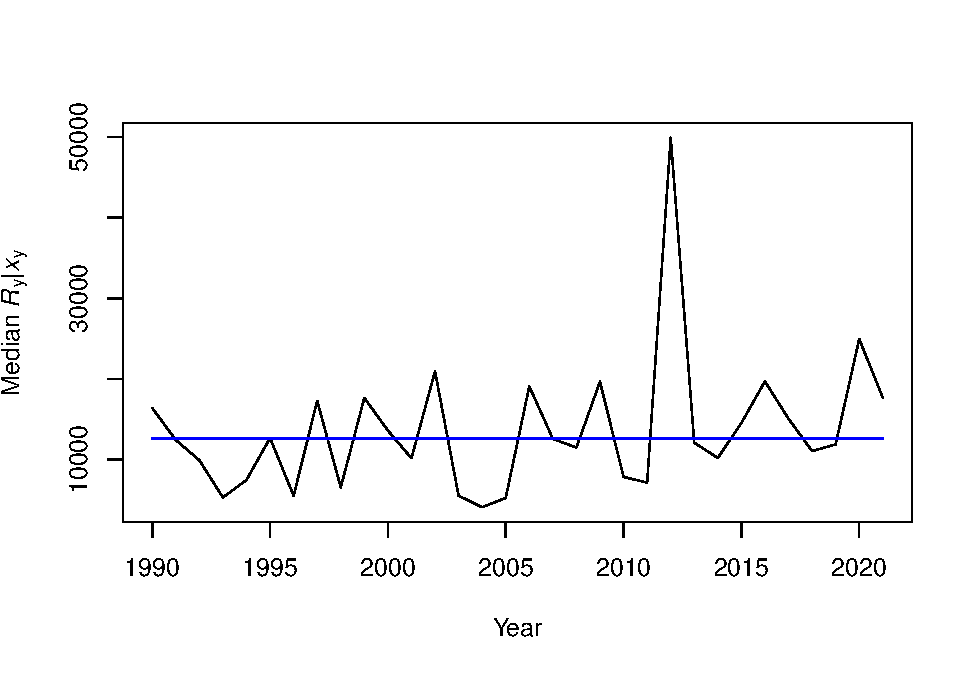
\includegraphics{bsb_models_wp_files/figure-latex/relative-recruitment-bt-1} 

}

\caption{Median recruitment with and without temperature ($x$) effects.}\label{fig:relative-recruitment-bt}
\end{figure}

\begin{figure}

{\centering 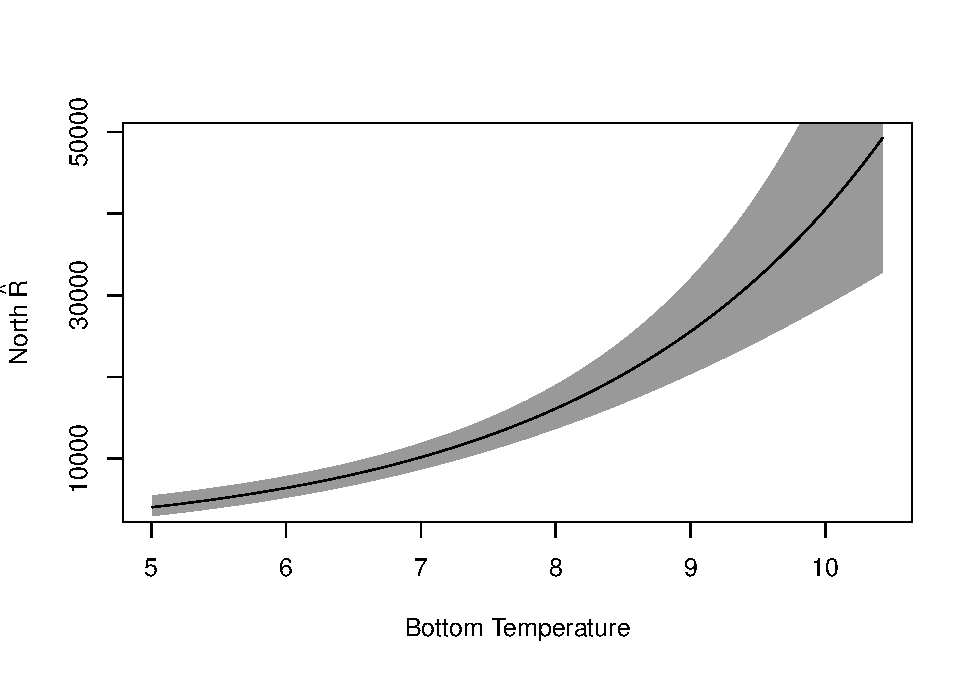
\includegraphics{bsb_models_wp_files/figure-latex/rec-bottom-temp-1} 

}

\caption{Expected recruitment for the northern component of the black sea bass stock as a function of bottom temperature}\label{fig:rec-bottom-temp}
\end{figure}

\begin{figure}

{\centering 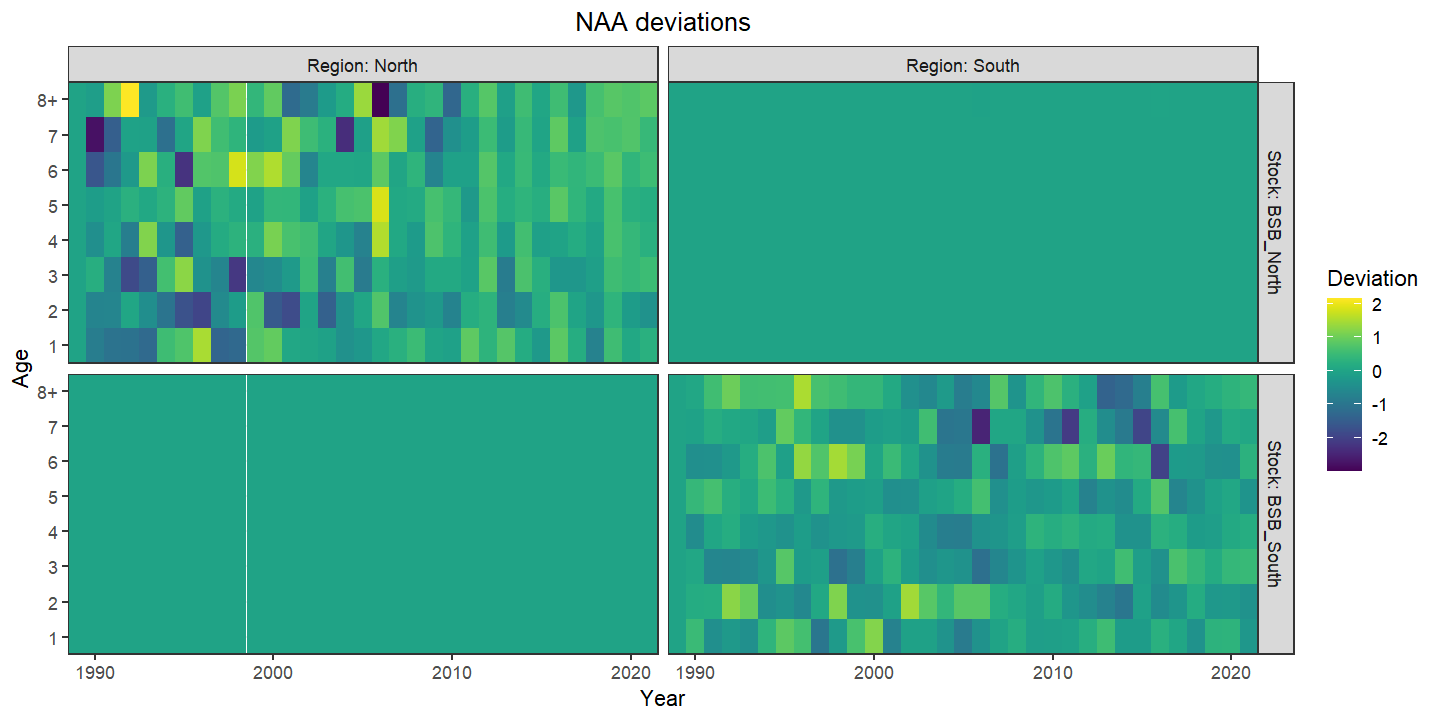
\includegraphics[width=1\linewidth]{../2023.RT.Runs/Run34/plots_png/results/NAA_dev_tile} 

}

\caption{Estimated survival deviations from the proposed base model.}\label{fig:NAA-devs}
\end{figure}

\begin{figure}

{\centering 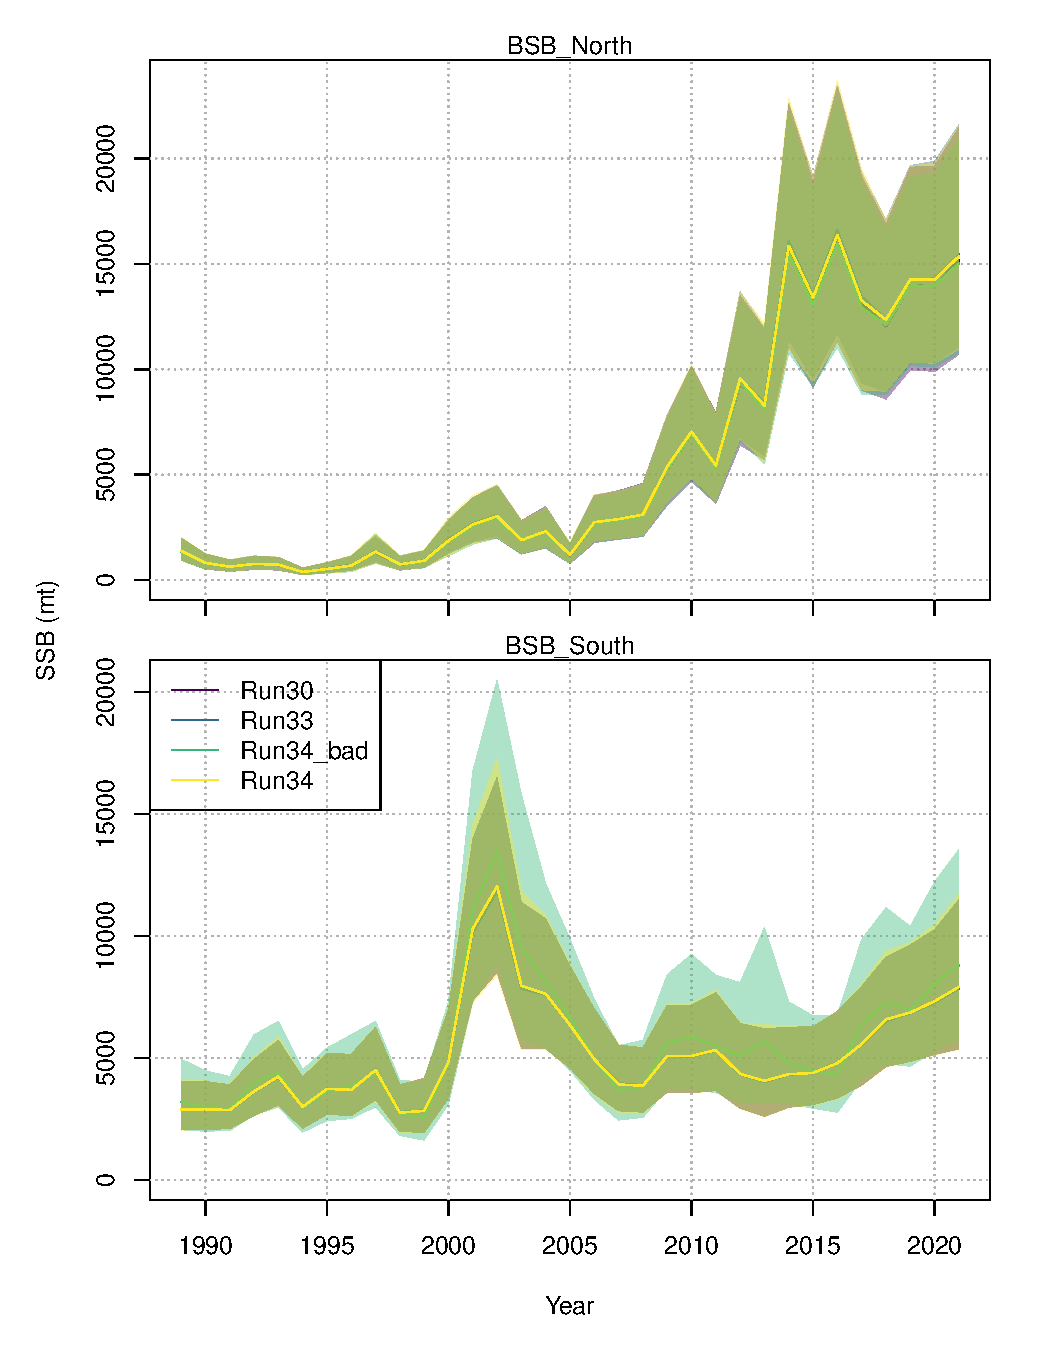
\includegraphics{bsb_models_wp_files/figure-latex/SSB-compare-1} 

}

\caption{Spawning stock biomass estimates from Runs 30, 33 and 34 (including the incorrect optimization). Polygons represent 95\% confidence intervals.}\label{fig:SSB-compare}
\end{figure}

\begin{figure}

{\centering 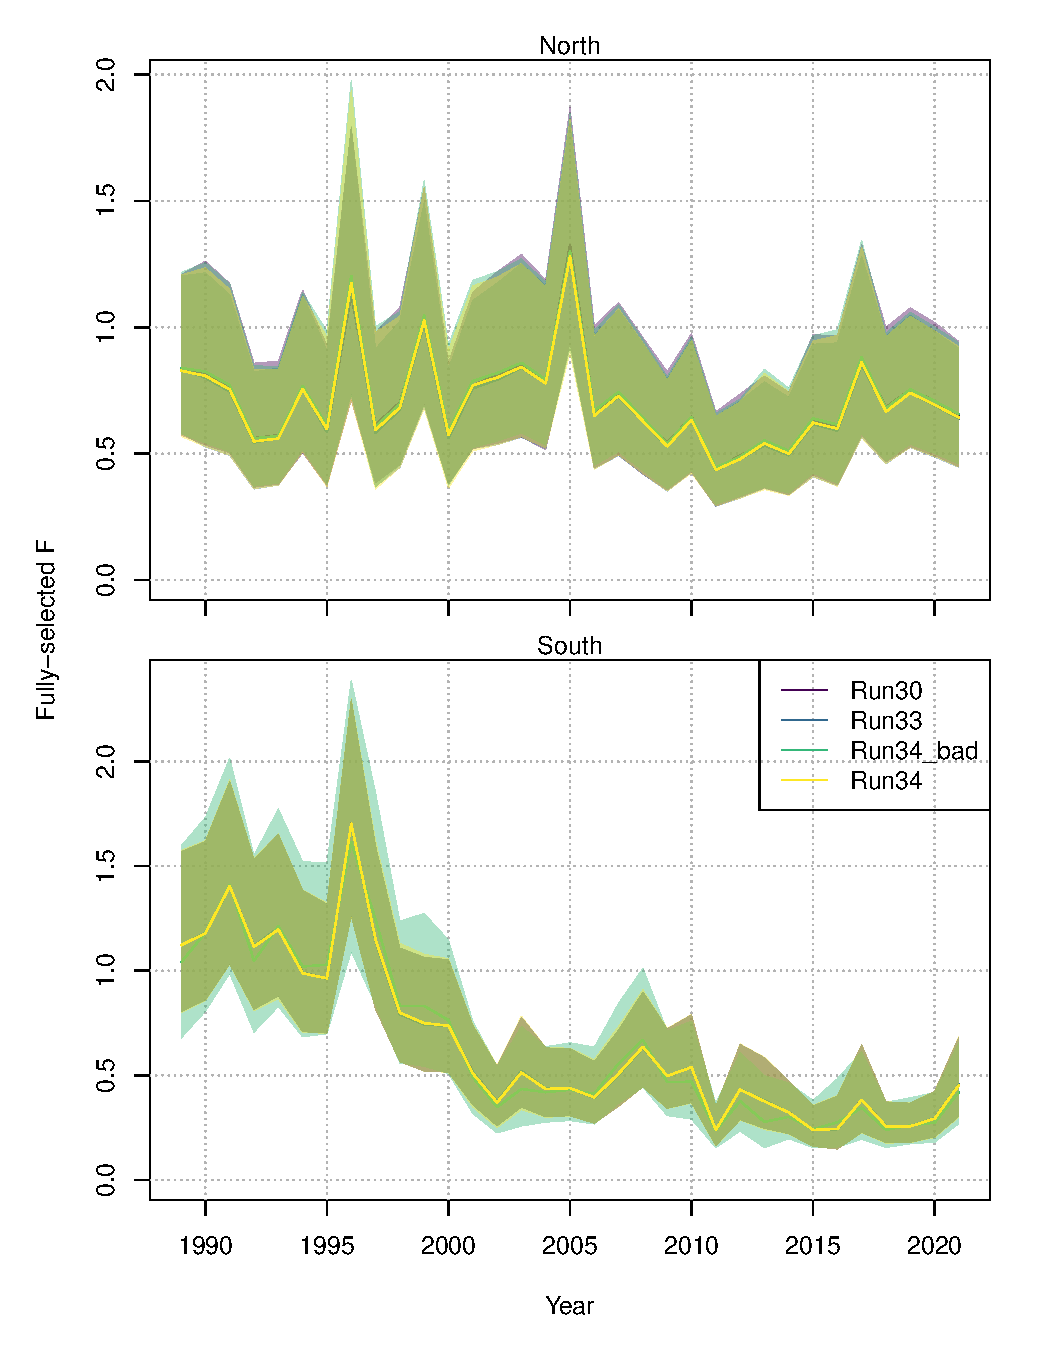
\includegraphics{bsb_models_wp_files/figure-latex/F-compare-1} 

}

\caption{Fully-selected fishing mortality estimates from Runs 30, 33 and 34 (including the incorrect optimization). Polygons represent 95\% confidence intervals.}\label{fig:F-compare}
\end{figure}

\begin{figure}

{\centering 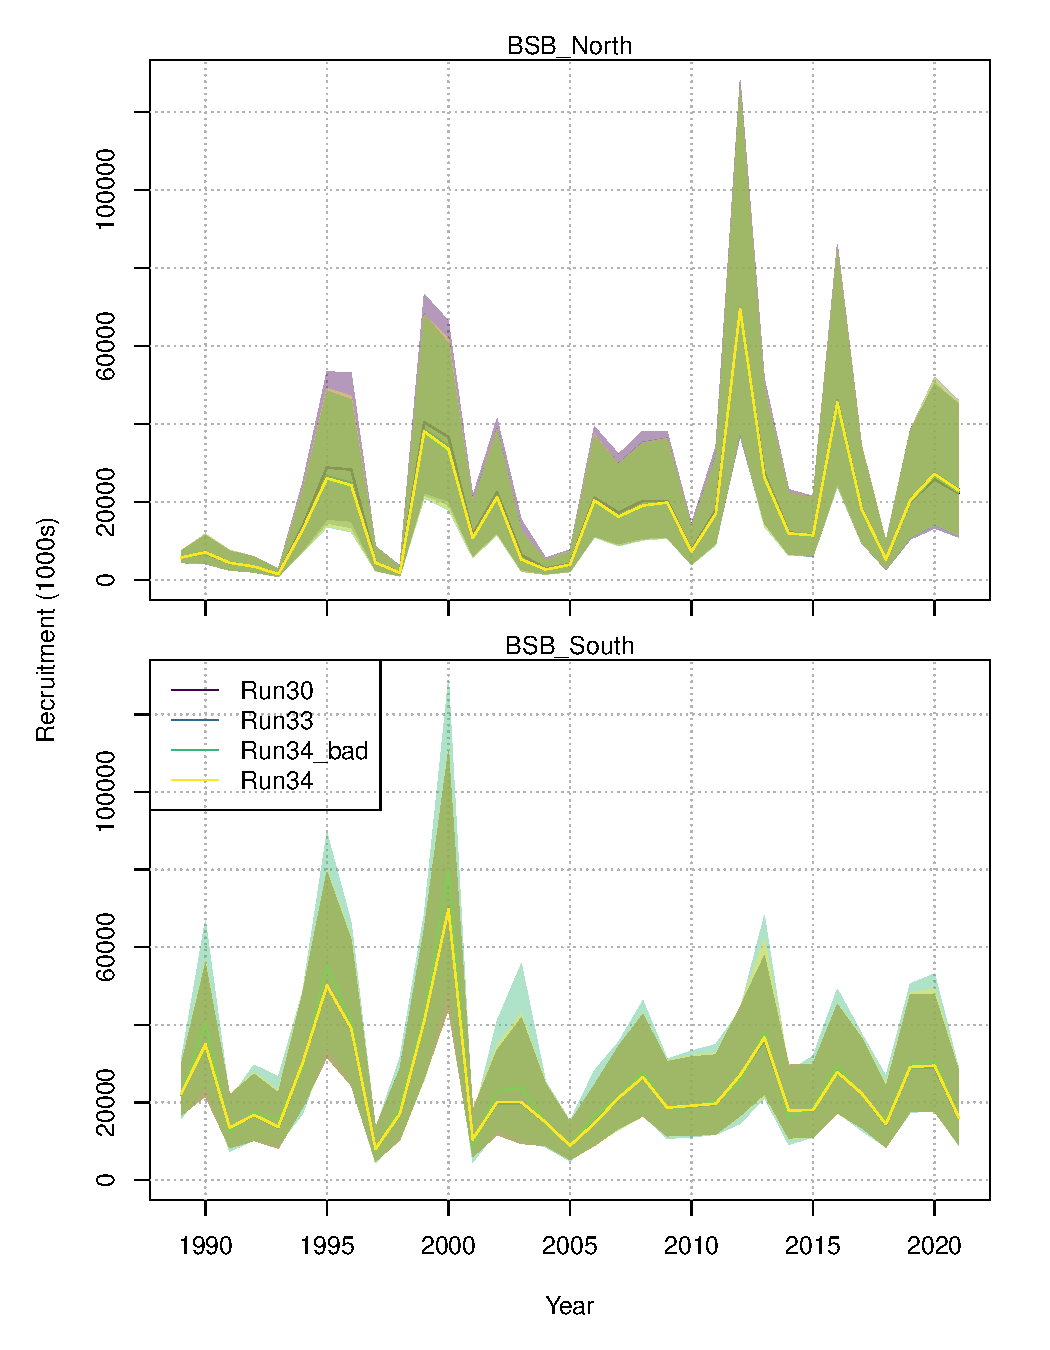
\includegraphics{bsb_models_wp_files/figure-latex/R-compare-1} 

}

\caption{Recruitment estimates from Runs 30, 33 and 34 (including the incorrect optimization). Polygons represent 95\% confidence intervals.}\label{fig:R-compare}
\end{figure}

\begin{figure}

{\centering 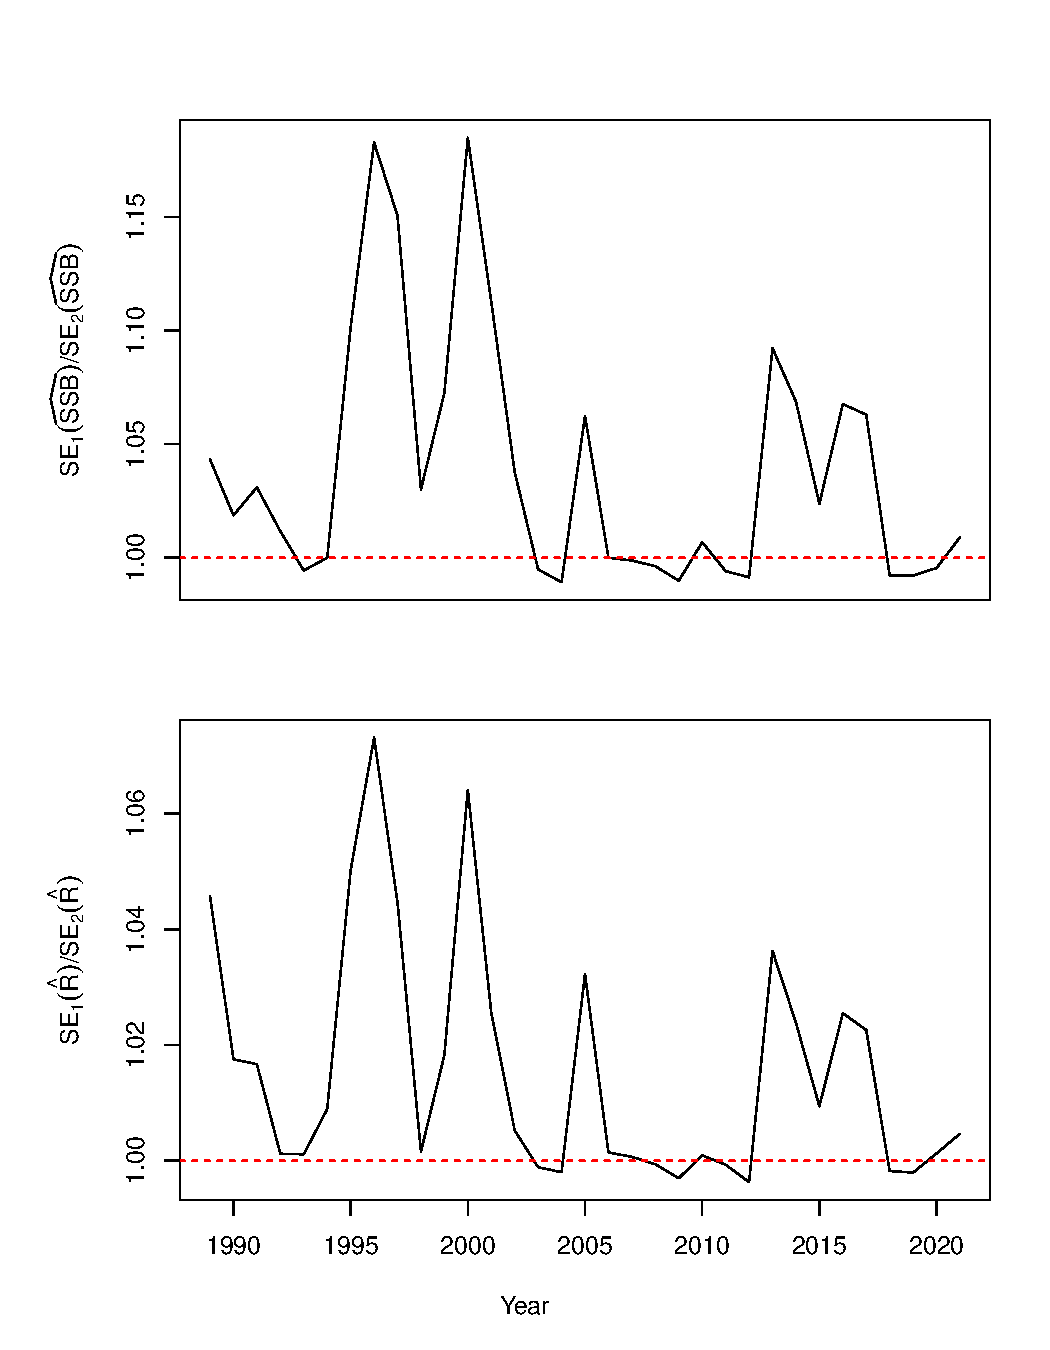
\includegraphics{bsb_models_wp_files/figure-latex/relative-se-ssb-R-1} 

}

\caption{Ratio of standard errors of Northern component SSB (top) and recruitment (bottom) for fitted models with ($SE_1$) and without ($SE_2$) the scalar of the Recreational CPA index standard errors estimated.}\label{fig:relative-se-ssb-R}
\end{figure}

\clearpage

\begin{figure}

{\centering 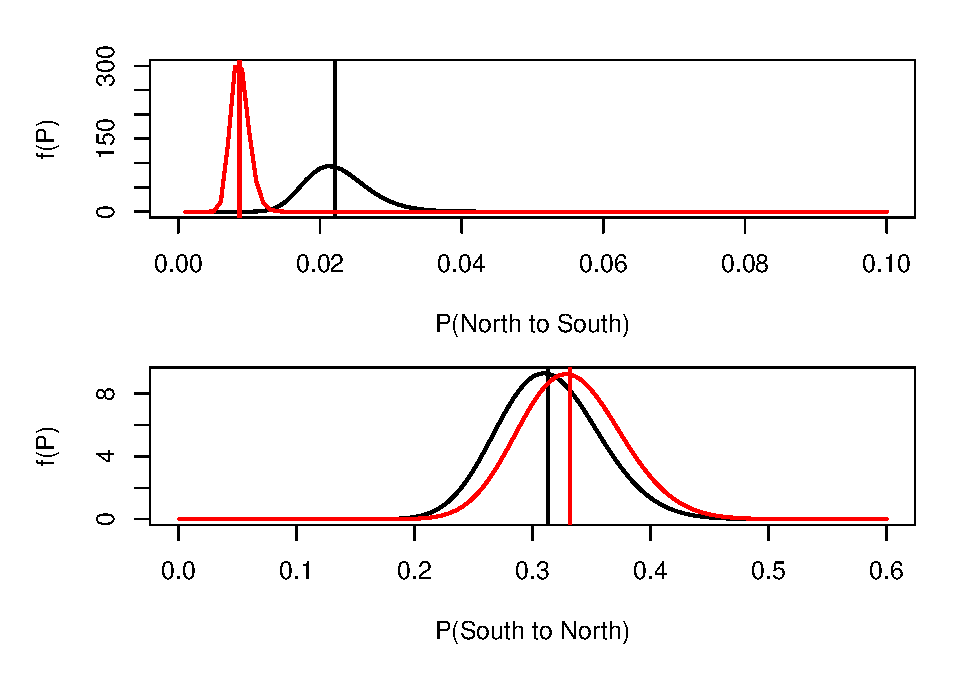
\includegraphics{bsb_models_wp_files/figure-latex/move-prior-posterior-1} 

}

\caption{Prior (black) and posterior (red) distributions of movement of northern component stock from north to south (top) and south to north (bottom)}\label{fig:move-prior-posterior}
\end{figure}

\clearpage
\begin{figure}

{\centering \includegraphics[width=1\linewidth]{../2023.RT.Runs/Run34/plots_png/results/SelAA_tile} 

}

\caption{Estimated selectivity for indices and fleets from the proposed base model.}\label{fig:selectivity}
\end{figure}

\begin{figure}

{\centering \includegraphics[width=0.65\linewidth]{../2023.RT.Runs/Run34/plots_png/results/SSB_Rec_time_BSB_North} \includegraphics[width=0.65\linewidth]{../2023.RT.Runs/Run34/plots_png/results/SSB_Rec_time_BSB_South} 

}

\caption{Estimated Spawning stock biomass and recruitment for the northern and southern components.}\label{fig:SSB-R-time}
\end{figure}

\begin{figure}

{\centering \includegraphics[width=1\linewidth]{../2023.RT.Runs/Run34/plots_png/results/SSB_F_trend} 

}

\caption{Estimated spawning stock biomass for regional components and fully-selected fishing mortalty for each region with 95\% confidence intervals. Polygons represents 95\% confidence intervals.}\label{fig:SSB-F}
\end{figure}
\clearpage

\begin{figure}

{\centering \includegraphics[width=1\linewidth]{../2023.RT.Runs/Run34/plots_png/results/F_byfleet} 

}

\caption{Estimated fully-selected fishing mortality for each fleet.}\label{fig:F-by-fleet}
\end{figure}

\begin{figure}

{\centering \includegraphics[width=1\linewidth]{../2023.RT.Runs/Run34/plots_png/ref_points/FSPR_absolute} 

}

\caption{Estimated equilibrium fully-selected fishing mortality, spawning stock biomass, and yield at 40\% of unfished spawning stock biomass per recruit. Annual values of inputs to per recruit calculations are used for the corresponding annual BRP estimates. Polygons represents 95\% confidence intervals.}\label{fig:annual-BRPs}
\end{figure}



\begin{figure}

{\centering \includegraphics[width=1\linewidth]{../2023.RT.Runs/Run34/plots_png/ref_points/FSPR_relative} 

}

\caption{Status of fishing mortality rates and spawning stock biomass relative to annual reference point estimates in Figure \ref{fig:annual-BRPs}. Gray polygon represents 95\textbackslash\% confidence intervals.}\label{fig:annual-status}
\end{figure}

\begin{figure}

{\centering \includegraphics[width=1\linewidth]{../2023.RT.Runs/Run34/plots_png/ref_points/Kobe_status} 

}

\caption{Kobe plot of status of fishing mortality and spawning stock biomass relative to corresponding reference point estimates ($F_{40}$ and $SSB(F_{40})$) using average of inputs to per-recruit calculations over 2017-2021. $SSB(F_{40})$ uses average recruitment from 2000 to 2021. Polygon represent a 95\% confidence region.}\label{fig:kobe-status}
\end{figure}

\clearpage

\begin{figure}

{\centering \includegraphics[width=0.65\linewidth]{../2023.RT.Runs/Run34/projections/plots_png/results/Ecov_1_North_BT} 

}

\caption{Observations and estimates of the bottom temperature covariates in the northern region from the proposed base model. Horizontal dashed line indicates when projection period begins.}\label{fig:bottom-temp-proj}
\end{figure}

\begin{figure}

{\centering \includegraphics[width=1\linewidth]{../2023.RT.Runs/Run34/projections/plots_png/results/NAA_dev_tile} 

}

\caption{Estimated survival deviations from the proposed base model. Horizontal dashed line indicates when projection period begins.}\label{fig:NAA-devs-proj}
\end{figure}

\begin{figure}

{\centering \includegraphics[width=0.65\linewidth]{../2023.RT.Runs/Run34/projections/plots_png/results/SSB_Rec_time_BSB_North} \includegraphics[width=0.65\linewidth]{../2023.RT.Runs/Run34/projections/plots_png/results/SSB_Rec_time_BSB_South} 

}

\caption{Estimated Spawning stock biomass and recruitment for the northern and southern components. Horizontal dashed line indicates when projection period begins.}\label{fig:SSB-R-time-proj}
\end{figure}

\begin{figure}

{\centering \includegraphics[width=1\linewidth]{../2023.RT.Runs/Run34/projections/plots_png/results/SSB_F_trend} 

}

\caption{Estimated spawning stock biomass for regional components and fully-selected fishing mortalty for each region with 95\% confidence intervals. Horizontal dashed line indicates when projection period begins.}\label{fig:SSB-F-proj}
\end{figure}
\clearpage

\begin{figure}

{\centering \includegraphics[width=1\linewidth]{../2023.RT.Runs/Run34/projections/plots_png/results/F_byfleet} 

}

\caption{Estimated fully-selected fishing mortality for each fleet. Horizontal dashed line indicates when projection period begins.}\label{fig:F-by-fleet-proj}
\end{figure}

\begin{figure}

{\centering \includegraphics[width=1\linewidth]{../2023.RT.Runs/Run34/projections/plots_png/ref_points/Kobe_status} 

}

\caption{Kobe plot of status of fishing mortality and spawning stock biomass relative to corresponding reference point estimates ($F_{40}$ and $SSB(F_{40})$) using average of inputs to per-recruit calculations over 2017-2021. $SSB(F_{40})$ uses average recruitment from 2000 to 2021. Polygons represent a 95\% confidence region.}\label{fig:kobe-status-proj}
\end{figure}

\clearpage

\begin{landscape}
\begin{longtable}[t]{l>{\raggedright\arraybackslash}p{10cm}>{\raggedright\arraybackslash}p{12cm}}
\caption{\label{tab:wham-runs}WHAM runs with description and comments.}\\
\toprule
Run & Description & Comments\\
\midrule
\endfirsthead
\caption[]{\label{tab:wham-runs}WHAM runs with description and comments. \textit{(continued)}}\\
\toprule
Run & Description & Comments\\
\midrule
\endhead

\endfoot
\bottomrule
\endlastfoot
1 & RE on recruitment and survival (iid). All indices with selectivities not flat topped at 2+ reexamined. Fleet selectivity (blocks, logistic) left as is. & Results in domed selectivity for several indices.\\
2 & Like Run 1, but removed blocking for recreational fleet and assumed iid time varying random effects on logistic parameters. & Does not converge. Variance of RE went to zero implying time-varying selectivity was not supported by data.\\
3 & Like Run 1, but estimated scalar multiplier for Rec CPA indices for north and south & Estimated multipliers were about 10 and 7 times for north and south input CVs.\\
4 & Like Run 3, but exchange all indices (other than Rec CPA) for VAST indices & Use bridge run 9 dat files\\
5 & Like Run 3, but remove all indices other than NEFSC, Rec CPA and NEAMAP & Use bridge run 6 dat files\\
\addlinespace
6 & Like Run 3, but exchange all indices (other than Rec CPA) for VAST indices (spring AND FALL) & Use bridge run 8 dat files\\
7 & Like Run 6, but switch age comp ll for all fleets, indices to logistic-normal-miss0 & re-examine selectivity for all indices\\
8 & Like Run 7, but assume movement from north to south and north to south for north pop during non spawning seasons at rates from synthesis model. & Had to fix CVs for Rec CPA indices and sigma for North 2+ survival at values from Run 7.\\
9 & Like Run 8, but use priors for movement with mean and sigma from synthesis model & Had to fix sigma for North 2+ survival like Run 8 and had to fix CVs for Rec CPA back to original smaller values.\\
10 & Like Run 9, but try estimating ar1 time-varying north-south movement & Does not coverge\\
\addlinespace
11 & Like Run 8, but include time-varying selectivity for VAST indices & Better AIC than Run 8\\
12 & Like Run 11, but try to estimate AR1 correlations for survival deviations & Does not coverge\\
13 & Like Run 11, but try to estimate M & Does not coverge\\
14 & Like Run 11, but use priors for movement rates instead of fixed & Does not coverge\\
15 & Like Run 8, but make selectivity logistic for everything & Does not coverge\\
\addlinespace
16 & like Run 8,  but simplify selectivities. Put selblock 5 back to logistic, simplify age-specific selectivities for Vast indices. Make Rec CPA logistic. & \\
17 & like Run 16, but use Dirichlet & \\
18 & Like Run 17, but set max age of fall VAST in North to age 1. & \\
19 & Just spring VAST and rec CPA as indices. Use Dirichlet. & An error was found error in fall VAST and NEAMAP age comps. Only Spring VAST and Rec CPA indices used from this run on.\\
20 & Like Run 19, but use Dirichlet-multinomial. & Expanded input sample sizes to 1000. Initially tried logistic normal with and without AR1 assumption, but those did not converge. OSA residuals look same as 19.\\
\addlinespace
21 & Like Run 20, but use ar1 time-varying selectivity for north vast index. & when used also for south vast index, did not converge\\
22 & like Run 19, but just "rec" NAA re, D-M age comp, and get to time-varying selectivity for all indices. & \\
23 & like Run 22, but include survival RE. & Tried 2dar1 correlation even with just North. there becomes a scale problem. Reverted back to none-time-varying selectivity but ar1 with age to keep the number of fixed effects down.\\
24 & Like Run 23, but trying time-varying movement rate for north-south. & Retro for north SSB is not good\\
25 & Like Run 24, but dirichlet instead of D-M. & \\
\addlinespace
26 & Like Run 25, but try rounded age comp. Not advised. & Does not coverge\\
27 & Like Run 25, but try time-varying selectivity on fleets. & Does not coverge\\
28 & Use selectivity and age comp based on examinations of separate runs for north and south in North.Runs and South.Runs & Big changes in selectivity and age comp model assumptions\\
29 & Run 28, but include movement (fixed parameters). & Has projections.\\
30 & Run 29, but use priors for movement parameters instead of fixed values. & Fine tune variance parameters for populations. I.e., North population in the south is set to be ~SCAA. 2dar1 now converges for north and south. Has projections. SSB40 now just uses avg recruitment from years 2000 onward.\\
\addlinespace
31 & Run 30, but estimate AR1 on north to south movement rate for north pop & Does not coverge\\
32 & Run 30, but estimate B-H SR curves for North and South Populations & Steepness goes to 1 for both components\\
33 & Run 30, but estimate temperature effects on north recruitment. & Also fits here with no effect (but temp included), temp effect on both north and south, but temp effect on NORTH is best.\\
34 & Run 33, but Estimate log Rec CPA index sd scalars. & Proposed base model\\*
\end{longtable}
\end{landscape}
\clearpage

\begin{landscape}\begin{table}

\caption{\label{tab:age-comp-sel-table}Configuration of Age composition likelihood, mean selectivity model, and selectivity random effects for each age composition data component in Run 34.}
\centering
\begin{tabular}[t]{llll}
\toprule
Data component & Age Composition Likelihood & Mean Selectivity model & Random effects configuration\\
\midrule
North Commercial & Dirichlet-Multinomial & age-specific (flat-topped at ages > 3) & 2D-AR1 (age and year)\\
North Recreational & Logistic-normal (0s as missing) & age-specific (flat-topped at ages > 6) & 2D-AR1 (age and year)\\
South Commercial & Logistic-normal (AR1, 0s as missing) & logistic & None\\
South Recreational & Logistic-normal (AR1, 0s as missing) & logistic & None\\
North Recreational CPA & Logistic-normal (0s as missing) & age-specific (flat-topped at ages > 1) & AR1 (year)\\
\addlinespace
North VAST & Dirichlet-Multinomial & age-specific (flat-topped at ages > 4) & 2D-AR1 (age and year)\\
South Recreational CPA & Logistic-normal (AR1, 0s as missing) & age-specific (flat-topped at ages > 2) & None\\
South VAST & Logistic-normal (AR1, 0s as missing) & age-specific (flat-topped at ages > 1) & None\\
\bottomrule
\end{tabular}
\end{table}
\end{landscape}

\clearpage

\begin{table}

\caption{\label{tab:compare-table}Comparison of AIC and estimates of standard deviation of recruitment for models without any temperature effects on recruitment, with just effects on the northern component, and with effects on both components for Run 33.}
\centering
\begin{tabular}[t]{lrr}
\toprule
  & AIC & North $\widehat{\sigma}_R$\\
\midrule
No effect & -1556.58 & 0.91\\
North temperature effect only & -1567.42 & 0.72\\
Both temperature effects & -1566.87 & 0.72\\
\bottomrule
\end{tabular}
\end{table}
\clearpage

\begin{landscape}
\begin{longtable}[t]{lrrrr}
\caption{\label{tab:par-table}Parameter estimates, standard errors, and confidence intervals for the proposed base model.}\\
\toprule
  & Estimate & Std. Error & 95\% CI lower & 95\% CI upper\\
\midrule
\endfirsthead
\caption[]{\label{tab:par-table}Parameter estimates, standard errors, and confidence intervals for the proposed base model. \textit{(continued)}}\\
\toprule
  & Estimate & Std. Error & 95\% CI lower & 95\% CI upper\\
\midrule
\endhead

\endfoot
\bottomrule
\endlastfoot
BSB North mean log(R) intercept & $6.009$ & $0.899$ & $4.247$ & $7.770$\\
BSB North in North NAA $\sigma$ (age 1) & $0.718$ & $0.101$ & $0.545$ & $0.945$\\
BSB North in North NAA $\sigma$ (ages 2-8+) & $0.807$ & $0.047$ & $0.721$ & $0.904$\\
BSB North in South NAA $\sigma$ (age 1) & $0.718$ & $0.101$ & $0.545$ & $0.945$\\
BSB North  in North  NAA AR1 $\rho$ age & $0.091$ & $0.094$ & $-0.095$ & $0.271$\\
\addlinespace
BSB North  in North  NAA AR1 $\rho$ year & $0.256$ & $0.079$ & $0.096$ & $0.404$\\
BSB South Mean Recruitment & $21252.124$ & $4468.181$ & $14074.738$ & $32089.604$\\
BSB South in North NAA $\sigma$ (age 1) & $0.518$ & $0.079$ & $0.384$ & $0.700$\\
BSB South in North NAA $\sigma$ (ages 2-8+) & $0.614$ & $0.070$ & $0.490$ & $0.769$\\
BSB South in South NAA $\sigma$ (age 1) & $0.518$ & $0.079$ & $0.384$ & $0.700$\\
\addlinespace
BSB South in South NAA $\sigma$ (ages 2-8+) & $0.614$ & $0.070$ & $0.490$ & $0.769$\\
BSB South  in North  NAA AR1 $\rho$ age & $-0.108$ & $0.114$ & $-0.323$ & $0.118$\\
BSB South  in North  NAA AR1 $\rho$ year & $0.318$ & $0.101$ & $0.109$ & $0.501$\\
BSB South  in South  NAA AR1 $\rho$ age & $-0.108$ & $0.114$ & $-0.323$ & $0.118$\\
BSB South  in South  NAA AR1 $\rho$ year & $0.318$ & $0.101$ & $0.109$ & $0.501$\\
\addlinespace
North REC CPA fully selected q & $1.020\times 10^{-4}$ & $1.502\times 10^{-5}$ & $7.641\times 10^{-5}$ & $1.361\times 10^{-4}$\\
North VAST Spring fully selected q & $0.016$ & $0.002$ & $0.012$ & $0.021$\\
South REC CPA fully selected q & $1.521\times 10^{-4}$ & $2.024\times 10^{-5}$ & $1.171\times 10^{-4}$ & $1.974\times 10^{-4}$\\
South VAST Spring fully selected q & $0.015$ & $0.002$ & $0.011$ & $0.019$\\
Block 1: North Commercial Mean Selectivity for age 1 & $0.019$ & $0.015$ & $0.004$ & $0.088$\\
\addlinespace
Block 1: North Commercial Mean Selectivity for age 2 & $0.326$ & $0.173$ & $0.094$ & $0.694$\\
Block 1: North Commercial Mean Selectivity for age 3 & $0.814$ & $0.128$ & $0.455$ & $0.958$\\
Block 1: North Commercial Mean Selectivity for age 4 & $1.000$ &  &  & \\
Block 1: North Commercial Mean Selectivity for age 5 & $1.000$ &  &  & \\
Block 1: North Commercial Mean Selectivity for age 6 & $1.000$ &  &  & \\
\addlinespace
Block 1: North Commercial Mean Selectivity for age 7 & $1.000$ &  &  & \\
Block 1: North Commercial Mean Selectivity for age 8+ & $1.000$ &  &  & \\
Block 2: North Recreational Mean Selectivity for age 1 & $0.029$ & $0.026$ & $0.005$ & $0.153$\\
Block 2: North Recreational Mean Selectivity for age 2 & $0.325$ & $0.199$ & $0.075$ & $0.740$\\
Block 2: North Recreational Mean Selectivity for age 3 & $0.558$ & $0.226$ & $0.173$ & $0.884$\\
\addlinespace
Block 2: North Recreational Mean Selectivity for age 4 & $0.787$ & $0.157$ & $0.371$ & $0.959$\\
Block 2: North Recreational Mean Selectivity for age 5 & $0.888$ & $0.097$ & $0.542$ & $0.981$\\
Block 2: North Recreational Mean Selectivity for age 6 & $0.950$ & $0.050$ & $0.709$ & $0.993$\\
Block 2: North Recreational Mean Selectivity for age 7 & $1.000$ &  &  & \\
Block 2: North Recreational Mean Selectivity for age 8+ & $1.000$ &  &  & \\
\addlinespace
Block 3: South Commercial $a_{50}$ & $2.465$ & $0.124$ & $2.229$ & $2.713$\\
Block 3: South Commercial 1/slope (increasing) & $0.401$ & $0.034$ & $0.340$ & $0.472$\\
Block 4: South Recreational $a_{50}$ & $2.843$ & $0.233$ & $2.405$ & $3.314$\\
Block 4: South Recreational 1/slope (increasing) & $0.822$ & $0.101$ & $0.645$ & $1.042$\\
Block 9: North REC CPA Mean Selectivity for age 1 & $0.158$ & $0.067$ & $0.065$ & $0.336$\\
\addlinespace
Block 9: North REC CPA Mean Selectivity for age 2 & $1.000$ &  &  & \\
Block 9: North REC CPA Mean Selectivity for age 3 & $1.000$ &  &  & \\
Block 9: North REC CPA Mean Selectivity for age 4 & $1.000$ &  &  & \\
Block 9: North REC CPA Mean Selectivity for age 5 & $1.000$ &  &  & \\
Block 9: North REC CPA Mean Selectivity for age 6 & $1.000$ &  &  & \\
\addlinespace
Block 9: North REC CPA Mean Selectivity for age 7 & $1.000$ &  &  & \\
Block 9: North REC CPA Mean Selectivity for age 8+ & $1.000$ &  &  & \\
Block 10: North VAST Spring Mean Selectivity for age 1 & $0.073$ & $0.027$ & $0.035$ & $0.148$\\
Block 10: North VAST Spring Mean Selectivity for age 2 & $0.403$ & $0.092$ & $0.242$ & $0.589$\\
Block 10: North VAST Spring Mean Selectivity for age 3 & $0.893$ & $0.060$ & $0.710$ & $0.966$\\
\addlinespace
Block 10: North VAST Spring Mean Selectivity for age 4 & $0.926$ & $0.039$ & $0.804$ & $0.975$\\
Block 10: North VAST Spring Mean Selectivity for age 5 & $1.000$ &  &  & \\
Block 10: North VAST Spring Mean Selectivity for age 6 & $1.000$ &  &  & \\
Block 10: North VAST Spring Mean Selectivity for age 7 & $1.000$ &  &  & \\
Block 10: North VAST Spring Mean Selectivity for age 8+ & $1.000$ &  &  & \\
\addlinespace
Block 11: South REC CPA Selectivity for age 1 & $0.399$ & $0.070$ & $0.273$ & $0.541$\\
Block 11: South REC CPA Selectivity for age 2 & $0.824$ & $0.076$ & $0.626$ & $0.929$\\
Block 11: South REC CPA Selectivity for age 3 & $1.000$ &  &  & \\
Block 11: South REC CPA Selectivity for age 4 & $1.000$ &  &  & \\
Block 11: South REC CPA Selectivity for age 5 & $1.000$ &  &  & \\
\addlinespace
Block 11: South REC CPA Selectivity for age 6 & $1.000$ &  &  & \\
Block 11: South REC CPA Selectivity for age 7 & $1.000$ &  &  & \\
Block 11: South REC CPA Selectivity for age 8+ & $1.000$ &  &  & \\
Block 12: South VAST Spring Selectivity for age 1 & $0.370$ & $0.080$ & $0.231$ & $0.535$\\
Block 12: South VAST Spring Selectivity for age 2 & $1.000$ &  &  & \\
\addlinespace
Block 12: South VAST Spring Selectivity for age 3 & $1.000$ &  &  & \\
Block 12: South VAST Spring Selectivity for age 4 & $1.000$ &  &  & \\
Block 12: South VAST Spring Selectivity for age 5 & $1.000$ &  &  & \\
Block 12: South VAST Spring Selectivity for age 6 & $1.000$ &  &  & \\
Block 12: South VAST Spring Selectivity for age 7 & $1.000$ &  &  & \\
\addlinespace
Block 12: South VAST Spring Selectivity for age 8+ & $1.000$ &  &  & \\
Block 1: North Commercial Selectivity RE $\sigma$ & $0.406$ & $0.116$ & $0.233$ & $0.710$\\
Block 1: North Commercial Selectivity RE AR1 $\rho$ (age) & $0.479$ & $0.138$ & $0.339$ & $0.940$\\
Block 1: North Commercial Selectivity RE AR1 $\rho$ (year) & $0.590$ & $0.082$ & $0.582$ & $0.967$\\
Block 2: North Recreational Selectivity RE $\sigma$ & $0.208$ & $0.030$ & $0.156$ & $0.277$\\
\addlinespace
Block 2: North Recreational Selectivity RE AR1 $\rho$ (age) & $0.519$ & $0.063$ & $0.650$ & $0.910$\\
Block 2: North Recreational Selectivity RE AR1 $\rho$ (year) & $0.733$ & $0.024$ & $0.874$ & $0.983$\\
Block 9: North REC CPA Selectivity RE $\sigma$ & $0.257$ & $0.067$ & $0.154$ & $0.428$\\
Block 9: North REC CPA Selectivity RE AR1 $\rho$ (year) & $0.659$ & $0.077$ & $0.543$ & $0.988$\\
Block 10: North VAST Spring Selectivity RE $\sigma$ & $0.745$ & $0.151$ & $0.501$ & $1.109$\\
\addlinespace
Block 10: North VAST Spring Selectivity RE AR1 $\rho$ (age) & $0.116$ & $0.249$ & $-0.276$ & $0.635$\\
Block 10: North VAST Spring Selectivity RE AR1 $\rho$ (year) & $0.341$ & $0.168$ & $0.182$ & $0.845$\\
North Commercial in North age comp, Dirichlet-multinomial: dispersion ($\phi$) & $54.899$ & $7.007$ & $42.749$ & $70.503$\\
North Recreational in North age comp, logistic-normal: $\sigma$ & $2.832$ & $0.337$ & $2.243$ & $3.576$\\
South Commercial in South age comp, logistic-normal: $\sigma$ & $33.924$ & $3.453$ & $27.789$ & $41.413$\\
\addlinespace
South Commercial in South age comp, logistic-normal: $\rho$ & $0.719$ & $0.061$ & $0.585$ & $0.823$\\
South Recreational in South age comp, logistic-normal: $\sigma$ & $27.914$ & $4.330$ & $20.596$ & $37.831$\\
South Recreational in South age comp, logistic-normal: $\rho$ & $0.910$ & $0.027$ & $0.842$ & $0.951$\\
North REC CPA in North age comp, logistic-normal: $\sigma$ & $4.301$ & $0.395$ & $3.592$ & $5.149$\\
North VAST Spring in North age comp, Dirichlet-multinomial: dispersion ($\phi$) & $28.550$ & $3.233$ & $22.868$ & $35.644$\\
\addlinespace
South REC CPA in South age comp, logistic-normal: $\sigma$ & $27.466$ & $4.520$ & $19.893$ & $37.921$\\
South REC CPA in South age comp, logistic-normal: $\rho$ & $0.927$ & $0.024$ & $0.864$ & $0.962$\\
South VAST Spring in South age comp, logistic-normal: $\sigma$ & $48.175$ & $3.878$ & $41.143$ & $56.408$\\
South VAST Spring in South age comp, logistic-normal: $\rho$ & $0.661$ & $0.057$ & $0.542$ & $0.762$\\
stock BSB North $\mu$ from North to South (intercept) & $0.009$ & $0.001$ & $0.006$ & $0.011$\\
\addlinespace
stock BSB North $\mu$ from South to North (intercept) & $0.332$ & $0.043$ & $0.253$ & $0.421$\\
North REC CPA log-index observation SD scalar & $4.736$ & $1.433$ & $2.618$ & $8.569$\\
South REC CPA log-index observation SD scalar & $5.306$ & $1.270$ & $3.319$ & $8.482$\\
Ecov North BT: $\mu$ & $6.803$ & $0.190$ & $6.431$ & $7.175$\\
Ecov North BT: $\sigma$ & $1.131$ & $0.109$ & $0.937$ & $1.367$\\
\addlinespace
Ecov North BT: AR1 $\rho$ & $0.290$ & $0.121$ & $0.040$ & $0.506$\\
Ecov South BT: $\mu$ & $7.606$ & $0.148$ & $7.316$ & $7.895$\\
Ecov South BT: $\sigma$ & $1.017$ & $0.092$ & $0.852$ & $1.215$\\
Ecov South BT: AR1 $\rho$ & $0.149$ & $0.124$ & $-0.099$ & $0.380$\\
BSB North Recruitment Ecov: North BT $\beta_1$ & $0.460$ & $0.117$ & $0.232$ & $0.688$\\*
\end{longtable}
\end{landscape}

\end{document}
